\documentclass[a4paper, oneside]{book}
\usepackage[utf8]{inputenc}
\usepackage[margin=3cm, bindingoffset=1cm]{geometry}
\linespread{1.5}
\usepackage{float}
\usepackage{csquotes}
\usepackage{subfig}
\usepackage{graphicx}
\usepackage{indentfirst}
\usepackage{fancyhdr}
\usepackage{array}
\usepackage[hidelinks]{hyperref}
\setlength{\parindent}{1cm}
\usepackage{tcolorbox}
\usepackage{makecell}
\usepackage{listings}
\usepackage{minted}
\usemintedstyle{manni}

% Definizione dell'ambiente lstlisting per il codice sorgente
\lstnewenvironment{code}[1][]%
    {\minipage{\linewidth} 
    \lstset{basicstyle=\ttfamily\footnotesize,frame=single,#1}}
    {\endminipage}

\pagestyle{fancy}
\renewcommand{\chaptermark}[1]{\markboth{\thechapter.\ \uppercase{#1}}{}}
\fancyhf{}
\fancyhead[C]{\textbf{\leftmark}}
\fancyfoot[C]{\thepage}
\renewcommand{\headrulewidth}{1pt}
\renewcommand{\footrulewidth}{1pt}
\usepackage[Conny]{fncychap}

\title{Embedded System Project}
\author{Group 7}
\date{May 2024}

\renewcommand{\contentsname}{\bf Indice}
\renewcommand{\chaptername}{Capitolo}
  
\begin{document}
    %Frontespizio
    \begin{titlepage}
        \begin{center}
            \LARGE{\uppercase{Università degli Studi di Salerno}}\\
            \vspace{5mm}
            %Dipartimento
        	\uppercase{\normalsize \textbf{Dipartimento di Ingegneria dell'Informazione ed Elettrica e Matematica Applicata} }\\
        \end{center}
        
        \begin{figure}[H]
            \centering
            
\includegraphics[width=0.35\textwidth]{logo_unisa}
        \end{figure}
        
        \begin{center}
            %Corso di Laurea
        	\normalsize{ Corso di Laurea Magistrale in Ingegneria Informatica }\\
        	\vspace{15mm}
        	%Titolo
            {\LARGE{\bf \uppercase{Warpex}}}\\
        	\vspace{3mm}
        \end{center}
        
        \vspace{15mm}

        \begin{center}
            \begin{tabular}{ | c | c | c | c |} \hline
                \textbf{Nome} & \textbf{Cognome} & \textbf{Matricola} & \textbf{E-Mail} \\ \hline
                    Michele & Martino & 0622702424 & m.martino48@studenti.unisa.it \\
                    \hline
                    Francesco & Quagliuolo & 0622702412 & f.quagliuolo@studenti.unisa.it \\
                    \hline
                    Emanuele & Relmi & 0622702368 & e.relmi@studenti.unisa.it \\
                    \hline
                    Benito & Senese & 0622702425 & b.senese1@studenti.unisa.it \\
                    \hline
                \end{tabular}
            \end{center}
        
        \vspace{20mm}
        
        %Anno Accademico
        \centering{\large \uppercase{ Anno Accademico 2023/2024 }}
    \end{titlepage}

    %Corpo della Tesi
    \tableofcontents
    \clearpage
    \sloppy
    \hyphenpenalty=10000
    \exhyphenpenalty=10000
    
    \chapter{\bf{User Stories}}

\section{US1 - Apertura Cancello}
\begin{tcolorbox}[title={Descrizione}, colback=red!20!white, colframe=red!80!black]
    \textbf{Come} utente, \\
    \textbf{voglio} premere il pulsante B1 quando il cancello è chiuso o in chiusura, \\
    \textbf{al fine di} avviare la fase di apertura del cancello.
\end{tcolorbox}

\begin{tcolorbox}[title={Criterio di Accettazione}, colback=blue!20!white, colframe=blue!80!black]
    \textbf{Dato che} il cancello è chiuso o in fase di chiusura, \\
    \textbf{quando} premo il pulsante B1, \\
    \textbf{allora} il cancello deve iniziare la fase di apertura.
\end{tcolorbox}

\section{US2 - Chiusura Cancello}
\begin{tcolorbox}[title={Descrizione}, colback=red!20!white, colframe=red!80!black]
    \textbf{Come} utente, \\
    \textbf{voglio} premere il pulsante B1 quando il cancello è in apertura o aperto, \\
    \textbf{al fine di} avviare la fase di chiusura del cancello.
\end{tcolorbox}

\begin{tcolorbox}[title={Criterio di Accettazione}, colback=blue!20!white, colframe=blue!80!black]
    \textbf{Dato che} il cancello è aperto o in fase di apertura, \\
    \textbf{quando} premo il pulsante B1, \\
    \textbf{allora} il cancello deve iniziare la fase di chiusura.
\end{tcolorbox}

\section{US3 - Regolazione Tempo Chiusura Automatica}
\begin{tcolorbox}[title={Descrizione}, colback=red!20!white, colframe=red!80!black]
    \textbf{Come} utente, \\
    \textbf{voglio} regolare il tempo di chiusura automatica del cancello premendo il pulsante B2 quando il cancello è chiuso, \\
    \textbf{al fine di} impostare dopo quanto tempo dall’apertura il cancello deve richiudersi.
\end{tcolorbox}

\begin{tcolorbox}[title={Criterio di Accettazione \#1}, colback=blue!20!white, colframe=blue!80!black]
    \textbf{Dato che} il cancello è chiuso, \\
    \textbf{quando} premo il pulsante B2, \\
    \textbf{se} il tempo di chiusura automatica è inferiore a 120 secondi, \\
    \textbf{allora} il tempo di chiusura automatica aumenta di 10 secondi.
\end{tcolorbox}

\begin{tcolorbox}[title={Criterio di Accettazione \#2}, colback=blue!20!white, colframe=blue!80!black]
    \textbf{Dato che} il cancello è chiuso, \\
    \textbf{quando} premo il pulsante B2, \\
    \textbf{se} il tempo di chiusura automatica è a 120 secondi, \\
    \textbf{allora} il tempo di chiusura automatica ritorna a 10 secondi.
\end{tcolorbox}

\section{US4 - Regolazione Tempo Lavoro}
\begin{tcolorbox}[title={Descrizione}, colback=red!20!white, colframe=red!80!black]
    \textbf{Come} utente, \\
    \textbf{voglio} regolare la durata delle fasi di apertura e chiusura del cancello premendo il pulsante B3 quando il cancello è chiuso, \\
    \textbf{al fine di} impostare la durata delle fasi di apertura e chiusura del cancello.
\end{tcolorbox}

\begin{tcolorbox}[title={Criterio di Accettazione \#1}, colback=blue!20!white, colframe=blue!80!black]
    \textbf{Dato che} il cancello è chiuso, \\
    \textbf{quando} premo il pulsante B3, \\
    \textbf{se} il tempo di lavoro è inferiore a 120 secondi, \\
    \textbf{allora} il tempo di lavoro aumenta di 10 secondi.
\end{tcolorbox}

\begin{tcolorbox}[title={Criterio di Accettazione \#2}, colback=blue!20!white, colframe=blue!80!black]
    \textbf{Dato che} il cancello è chiuso, \\
    \textbf{quando} premo il pulsante B3, \\
    \textbf{se} il tempo di lavoro è 120 secondi, \\
    \textbf{allora} il tempo di lavoro ritorna a 10 secondi.
\end{tcolorbox}

\section{US5 - Riapertura Automatica con Rilevazione Ostacolo}
\begin{tcolorbox}[title={Descrizione}, colback=red!20!white, colframe=red!80!black]
    \textbf{Come} utente, \\
    \textbf{voglio} che il cancello si riapra automaticamente se viene rilevata la presenza di un ostacolo durante la fase di chiusura, \\
    \textbf{in modo da} evitare danni al cancello e garantire la sicurezza delle persone e degli oggetti presenti.
\end{tcolorbox}

\begin{tcolorbox}[title={Criterio di Accettazione}, colback=blue!20!white, colframe=blue!80!black]
    \textbf{Dato che} il cancello è in fase di chiusura, \\
    \textbf{quando} il sensore di presenza (P1) rileva un ostacolo, \\
    \textbf{allora} il cancello si riapre automaticamente.
\end{tcolorbox}

\section{US6 - Gestione Sicura del Cancello in Presenza di Ostacoli}
\begin{tcolorbox}[title={Descrizione}, colback=red!20!white, colframe=red!80!black]
    \textbf{Come} utente, \\
    \textbf{voglio} che il dispositivo ignori le richieste di apertura o chiusura del cancello quando il sensore di presenza è attivo, \\
    \textbf{in modo da} prevenire movimenti non sicuri del cancello in presenza di ostacoli o persone.
\end{tcolorbox}

\begin{tcolorbox}[title={Criterio di Accettazione \#1}, colback=blue!20!white, colframe=blue!80!black]
    \textbf{Dato che} il sensore di presenza (P1) è attivo, \\
    \textbf{quando} c'è una richiesta di apertura o chiusura del cancello, \\
    \textbf{allora} il dispositivo non esegue l'azione richiesta.
\end{tcolorbox}

\begin{tcolorbox}[title={Criterio di Accettazione \#2}, colback=blue!20!white, colframe=blue!80!black]
    \textbf{Dato che} il sensore di presenza (P1), \\
    \textbf{quando} non rileva più alcun ostacolo, \\
    \textbf{allora} il dispositivo è nuovamente pronto a ricevere e gestire le richieste di apertura o chiusura del cancello..
\end{tcolorbox}

\section{US7 - Gestione del sensore di chiusura per determinare lo stato del cancello}
\begin{tcolorbox}[title={Descrizione}, colback=red!20!white, colframe=red!80!black]
    \textbf{Come} utente, \\
    \textbf{voglio} che il dispositivo utilizzi il sensore di presenza (P2) come sensore di chiusura del cancello\\
    \textbf{in modo da} determinare in modo affidabile lo stato del cancello.
\end{tcolorbox}

\begin{tcolorbox}[title={Criterio di Accettazione}, colback=blue!20!white, colframe=blue!80!black]
    \textbf{Dato che} il cancello è chiuso, \\
    \textbf{quando} il sensore di presenza (P2) è attivo, \\
    \textbf{allora} il cancello si considera chiuso.
\end{tcolorbox}

\section{US8 - Errore in caso di malfunzionamento del sensore di chiusura}
\begin{tcolorbox}[title={Descrizione}, colback=red!20!white, colframe=red!80!black]
    \textbf{Come} utente\\
    \textbf{voglio} che il dispositivo entri in uno stato di errore se il sensore di chiusura (P2) non si attiva dopo il tempo di lavoro previsto durante la fase di chiusura del cancello,\\
    \textbf{in modo da} essere avvisato in caso di malfunzionamento del sensore.
\end{tcolorbox}

\begin{tcolorbox}[title={Criterio di Accettazione}, colback=blue!20!white, colframe=blue!80!black]
    \textbf{Dato che} è in corso la fase di chiusura del cancello, \\
    \textbf{quando} il sensore di chiusura (P2) non si attiva entro il tempo di lavoro previsto, \\
    \textbf{allora} il dispositivo entra in uno stato di errore.
\end{tcolorbox}

\section{US9 - Avvio Chiusura Cancello senza Sensore Attivo}
\begin{tcolorbox}[title={Descrizione}, colback=red!20!white, colframe=red!80!black]
    \textbf{Come} utente, \\
    \textbf{voglio} che il dispositivo avvii la procedura di chiusura del cancello quando viene acceso, se il sensore di chiusura (P2) e il sensore di presenza (P1) non sono attivi, \\
    \textbf{in modo da} garantire la chiusura corretta del cancello all'accensione.
\end{tcolorbox}

\begin{tcolorbox}[title={Criterio di Accettazione}, colback=blue!20!white, colframe=blue!80!black]
    \textbf{Dato che} il dispositivo è acceso, \\
    \textbf{quando} il sensore di chiusura (P2) e il sensore di presenza (P1) non sono attivi, \\
    \textbf{allora} viene avviata la procedura di chiusura del cancello.
\end{tcolorbox}

\section{US10 - Indicazione del Cancello in Movimento}
\begin{tcolorbox}[title={Descrizione}, colback=red!20!white, colframe=red!80!black]
    \textbf{Come} utente, \\
    \textbf{voglio} che il LED giallo lampeggi mentre il cancello è in apertura o in chiusura, \\
    \textbf{al fine di} avere una conferma visiva dello stato di movimento.
\end{tcolorbox}

\begin{tcolorbox}[title={Criterio di Accettazione}, colback=blue!20!white, colframe=blue!80!black]
    \textbf{Dato} che il cancello è in fase di apertura o chiusura, \\
    \textbf{quando} il cancello si muove, \\
    \textbf{allora} il LED giallo lampeggia con una frequenza di 0,5 Hz.
\end{tcolorbox}

\section{US11 - Indicazione di Errore di Chiusura}
    \begin{tcolorbox}[title={Descrizione}, colback=red!20!white, colframe=red!80!black]
    \textbf{Come} utente, \\
    \textbf{voglio} che il LED rosso si accenda se il cancello non si chiude entro 10 secondi dal completamento del tempo di lavoro, \\
    \textbf{al fine di} essere notificato di uno stato di errore.
\end{tcolorbox}

\begin{tcolorbox}[title={Criterio di Accettazione}, colback=blue!20!white, colframe=blue!80!black]
    \textbf{Dato} che il cancello è in fase di chiusura, \\
    \textbf{quando} il cancello non si chiude entro 10 secondi dal completamento del tempo di lavoro, \\
    \textbf{allora} il LED rosso si accende per notificare lo stato di errore.
\end{tcolorbox}

\section{US12 - Indicazione di Ostacolo}
\begin{tcolorbox}[title={Descrizione}, colback=red!20!white, colframe=red!80!black]
    \textbf{Come} utente, \\
    \textbf{voglio} che il LED verde lampeggi se un ostacolo è presente davanti al sensore P1 quando si richiede l'apertura o la chiusura, \\
    \textbf{al fine di} essere notificato della presenza di un ostacolo.
\end{tcolorbox}

\begin{tcolorbox}[title={Criterio di Accettazione}, colback=blue!20!white, colframe=blue!80!black]
    \textbf{Dato} che il cancello è completamente aperto o chiuso, \\
    \textbf{quando} un ostacolo è presente davanti al sensore P1 e si richiede l'apertura o la chiusura del cancello, \\
    \textbf{allora} il LED verde lampeggia con una frequenza di 1 Hz per 30 secondi.
\end{tcolorbox}

\section{US13 - Indicazione Cancello Chiuso}
\begin{tcolorbox}[title={Descrizione}, colback=red!20!white, colframe=red!80!black]
    \textbf{Come} utente, \\
    \textbf{voglio} che tutti i LED siano spenti quando il cancello è chiuso, \\
    \textbf{al fine di} avere una conferma visiva che il cancello è completamente chiuso.
\end{tcolorbox}

\begin{tcolorbox}[title={Criterio di Accettazione}, colback=blue!20!white, colframe=blue!80!black]
    \textbf{Dato} che la procedura di chiusura del cancello è attiva, \\
    \textbf{quando} il cancello è completamente chiuso, \\
    \textbf{allora} tutti i LED sono spenti.
\end{tcolorbox}

\section{US14 - Indicazione Cancello Aperto}
\begin{tcolorbox}[title={Descrizione}, colback=red!20!white, colframe=red!80!black]
    \textbf{Come} utente, \\
    \textbf{voglio} che tutti i LED siano accesi senza lampeggiare quando il cancello è aperto, \\
    \textbf{al fine di} avere una conferma visiva che il cancello è completamente aperto.
\end{tcolorbox}

\begin{tcolorbox}[title={Criterio di Accettazione}, colback=blue!20!white, colframe=blue!80!black]
    \textbf{Dato} che la procedura di apertura del cancello è attiva, \\
    \textbf{quando} il cancello è completamente aperto, \\
    \textbf{allora} tutti i LED sono accesi senza lampeggiare.
\end{tcolorbox}
    \chapter{\bf{Use Cases}}
\noindent Per poter rappresentare le user stories sopra descritte, utilizziamo gli Use Case Diagrams, dei diagrammi che rappresentano le interazioni tra gli utenti e il sistema.
In questo scenario, l'attore principale è l'utente che  interagisce con il sistema del cancello automatico attraverso i pulsanti B1, B2 e B3.


\section{Apertura Cancello [US1-US10-US14]}
L'utente ha la possibilità, in prossimità del cancello, di richiederne l'apertura premendo il pulsante B1. Quando il sistema rileva che il pulsante B1 è stato premuto e il cancello è nelle condizioni specificate (chiuso o in chiusura), avvia il processo di apertura del cancello. Il dispositivo inoltre fornisce un feedback visivo data dall'attivazione di un segnale luminoso, dato dal lampeggiamento di un LED giallo con frequenza 0.5 Hz.
Il dispositivo, inoltre, permette di verificare la completa apertura del cancello tramite l'accensione di tutti i LED: giallo, rosso e verde (figura \ref{usecase1}).

\begin{figure}
    \centering
    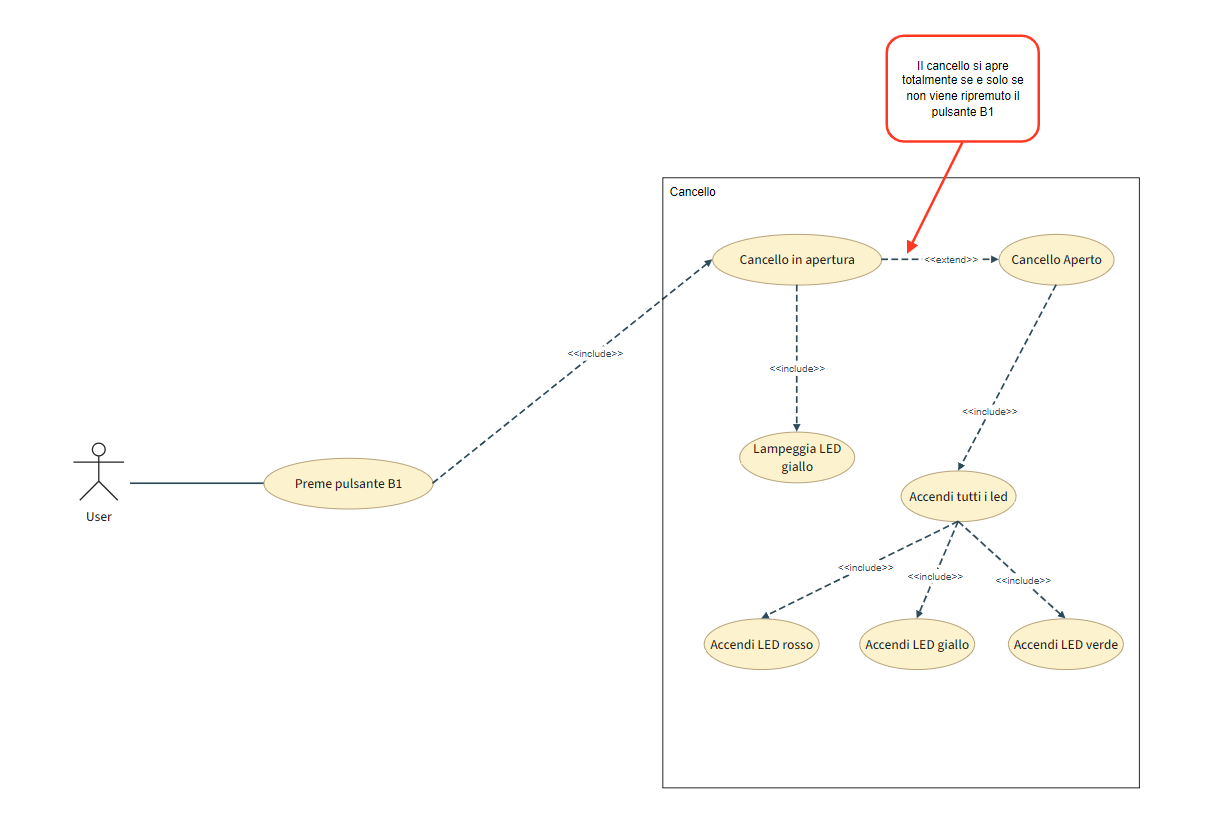
\includegraphics[width=0.9\textwidth]{figures/usecase_1.png}
    \caption{Apertura Cancello}
    \label{usecase1}
\end{figure}


\section{Chiusura Cancello [US2-US10-US13]}
L'utente ha la possibilità, in prossimità del cancello, di richiederne la chiusura premendo il pulsante B1. Quando il sistema rileva che il pulsante B1 è stato premuto e il cancello è nelle condizioni specificate (aperto o in apertura), avvia il processo di chiusura del cancello. Il dispositivo inoltre fornisce un feedback visivo data dall'attivazione di un segnale luminoso, dato dal lampeggiamento di un LED giallo con frequenza 0.5 Hz.
Il dispositivo, inoltre, permette di verificare la completa chiusura del cancello tramite lo spegnimento di tutti i LED (figura \ref{usecase2}).

\begin{figure}[H]
    \centering
    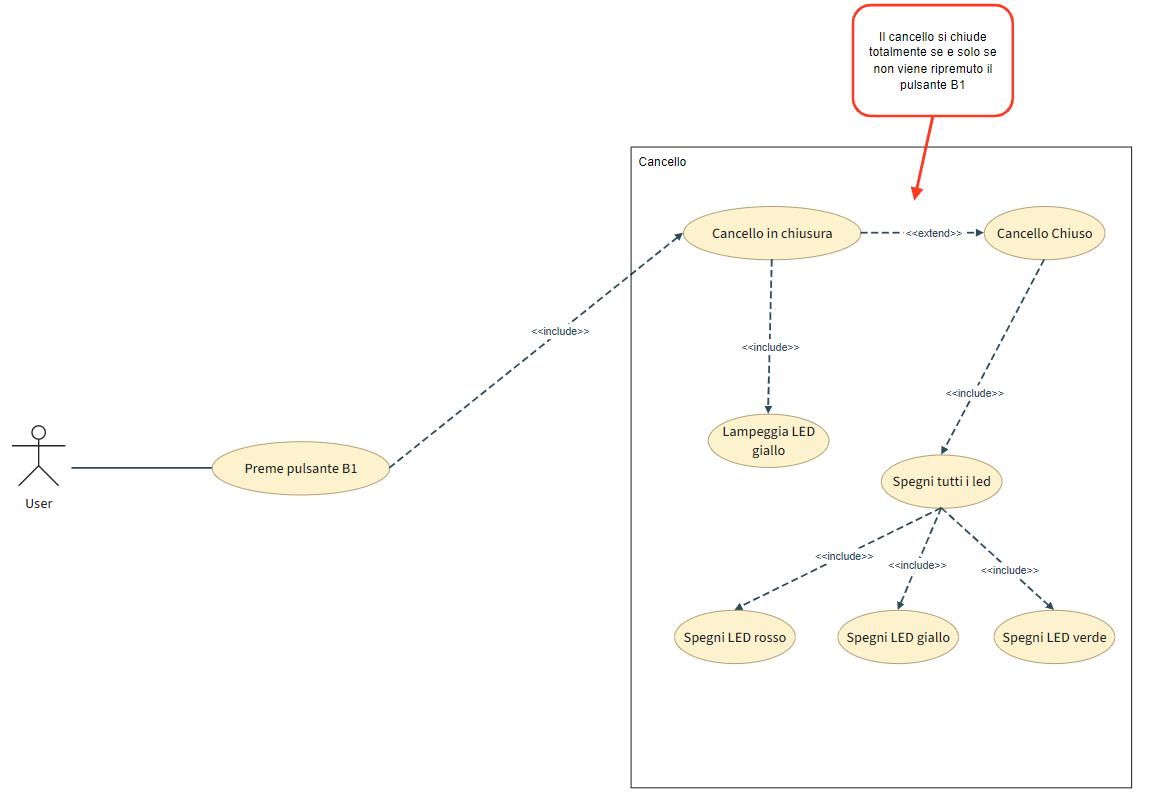
\includegraphics[width=0.9\textwidth]{figures/usecase_2.png}
    \caption{Chiusura Cancello}
    \label{usecase2}
\end{figure}


\section{Regolazione tempo di chiusura automatica [US3]}
L'utente ha la possibilità di regolare il tempo di chiusura automatica del cancello andando a determinare quanto esso debba rimanere aperto prima di chiudersi automaticamente.
Quando il cancello è chiuso, l'utente preme il pulsante B2 per effettuare la regolazione. Se il tempo di chiusura automatica è inferiore a 120 secondi, ogni pressione del pulsante B2 aumenta il tempo di 10 secondi. Se il tempo è già a 120 secondi, premendo nuovamente B2 il tempo viene riportato a 10 secondi (\ref{usecase3}).


\section{Regolazione Tempo di Lavoro [US4]}
L'utente ha la possibilità  di richiedere la regolazione della durata della fasi di apertura e chiusura del cancello premendo l'apposito pulsante (B3) solo quando il cancello è chiuso. Questa azione è essenziale per impostare la durata delle due fasi del cancello. Ogni pressione del pulsante incrementa la durata di 10 secondi e, se il tempo di lavoro è al suo massimo (120 secondi), esso ritorna a 10 secondi (\ref{usecase3}).

\begin{figure}[H]
    \centering
    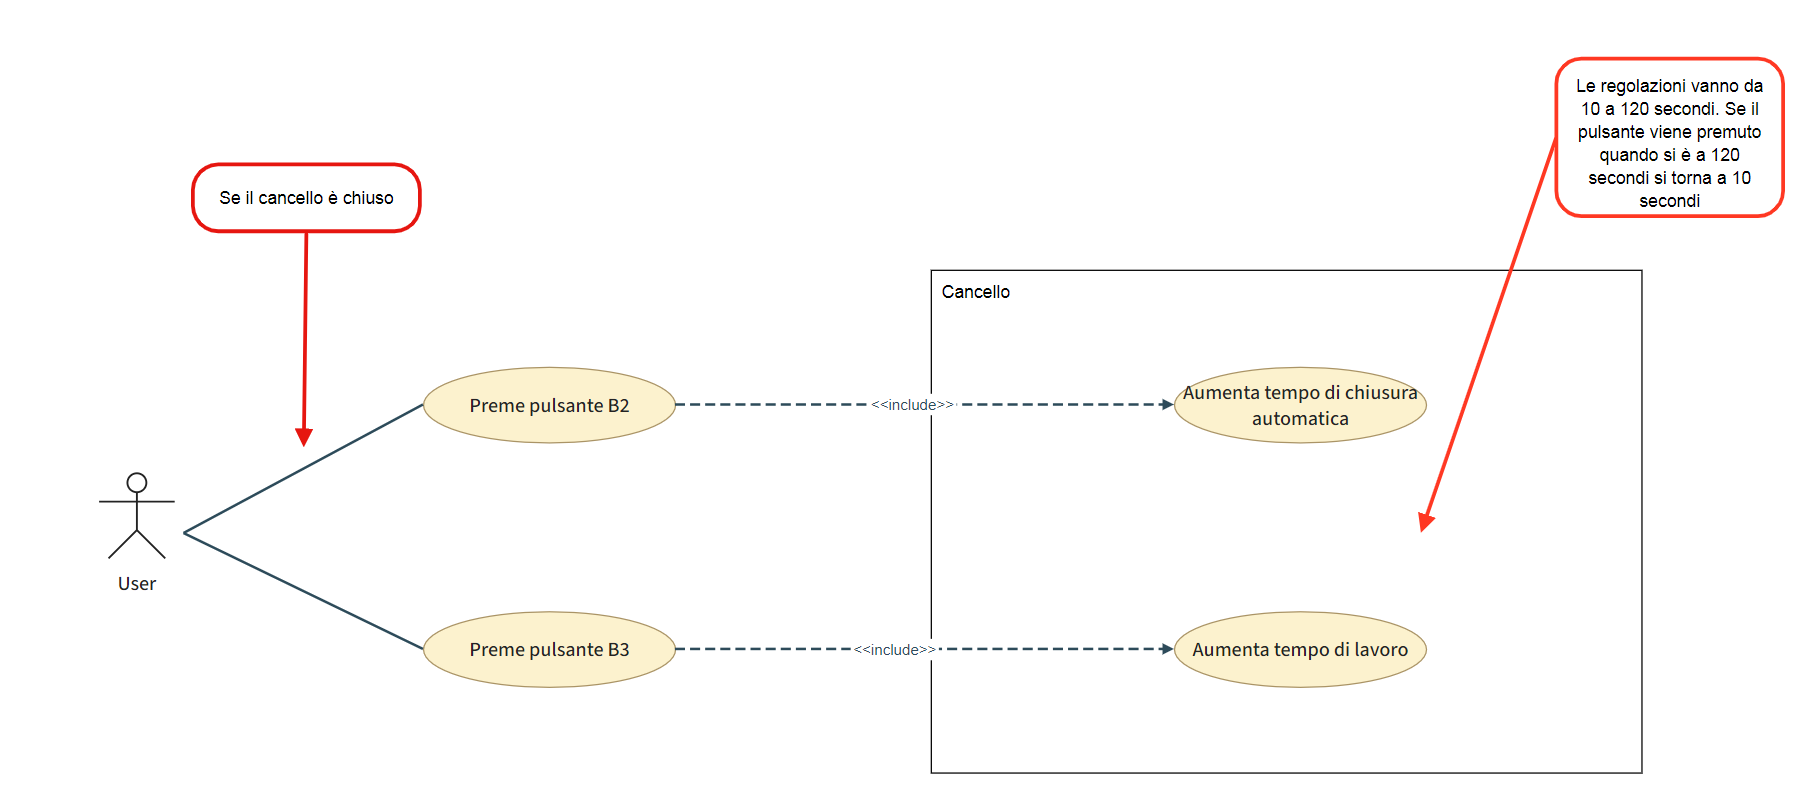
\includegraphics[width=0.9\textwidth]{figures/usecase_3.png}
    \caption{Regolazioni}
    \label{usecase3}
\end{figure}


\section{Riapertura Automatica con Rilevazione Ostacolo [US5-US14]}
L'utente ha la possibilità di richiedere la riapertura automatica del cancello se viene rilevata la presenza di un ostacolo durante la fase di chiusura tramite un sensore di presenza (P1). Questa azione è essenziale per evitare danni al cancello e garantire la sicurezza delle persone e degli oggetti presenti. 
Il dispositivo fornisce un feedback in caso di apertura completa del cancello, dato dall'accensione di tutti i LED (\ref{usecase5}).


\section{Gestione Richieste in presenza di ostacoli [US6-US12]}
L'utente ha la possibilità di richiedere che il dispositivo ignori le richieste di apertura o chiusura del cancello quando il sensore di presenza P1 è attivo. Questa azione è essenziale per prevenire movimenti non sicuri del cancello in presenza di ostacoli o persone.
Il dispositivo fornisce un feedback visivo in caso di presenza di un ostacolo, dato dal lampeggio del LED verde con frequenza di 1 Hz per un tempo di 30 secondi (\ref{usecase5}).


\begin{figure}[H]
    \centering
    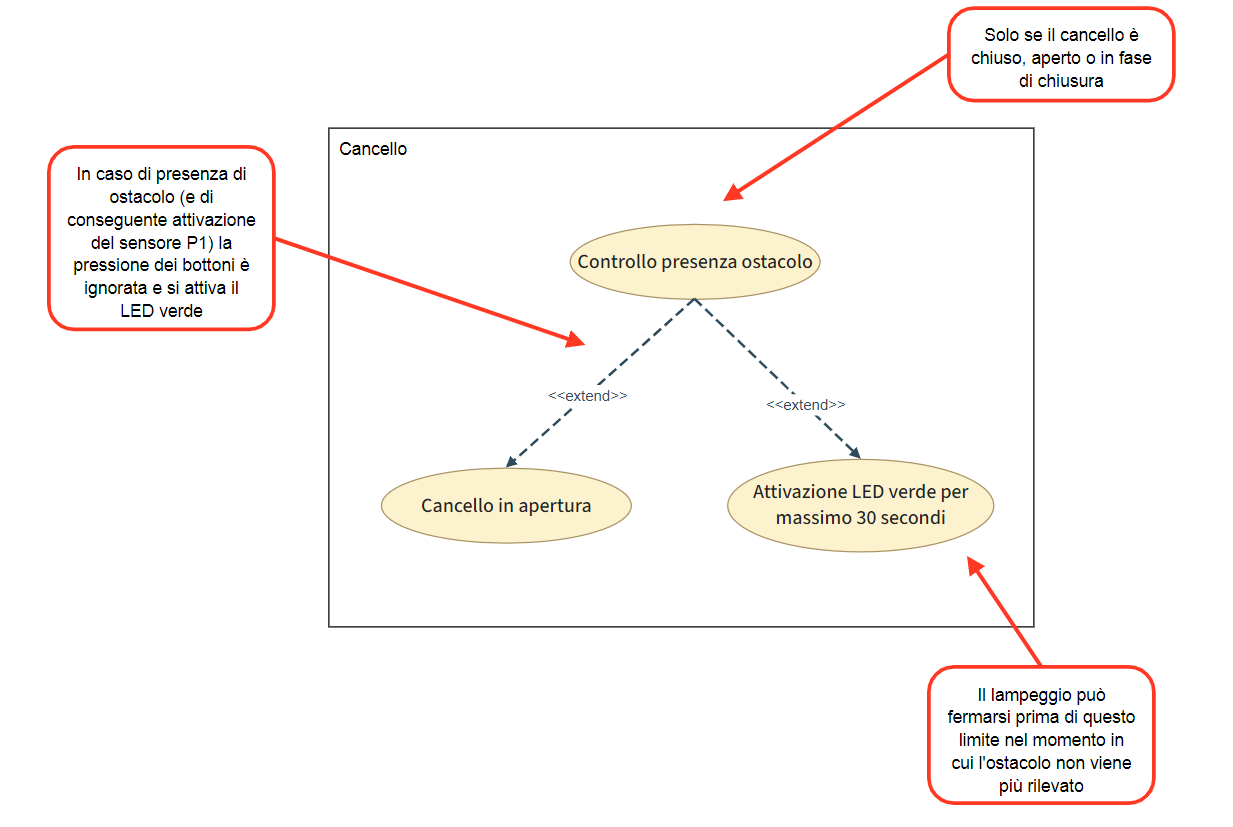
\includegraphics[width=0.9\textwidth]{figures/usecase_5.png}
    \caption{Controllo Ostacolo e Gestione Richieste}
    \label{usecase5}
\end{figure}


\section{Determinazione e Comunicazione stato cancello [US7-US13]}
L'utente ha la possibilità di richiedere la determinazione dello stato del cancello tramite un sensore di presenza (P2). Questa azione è essenziale per determinare correttamente lo stato del cancello che si considera chiuso quando il sensore è attivo (\ref{usecase7}). 
Il dispositivo fornisce un feedback visivo in caso il cancello risulti completamente chiuso, dato dallo spegnimento di tutti i LED.

\begin{figure}[H]
    \centering
    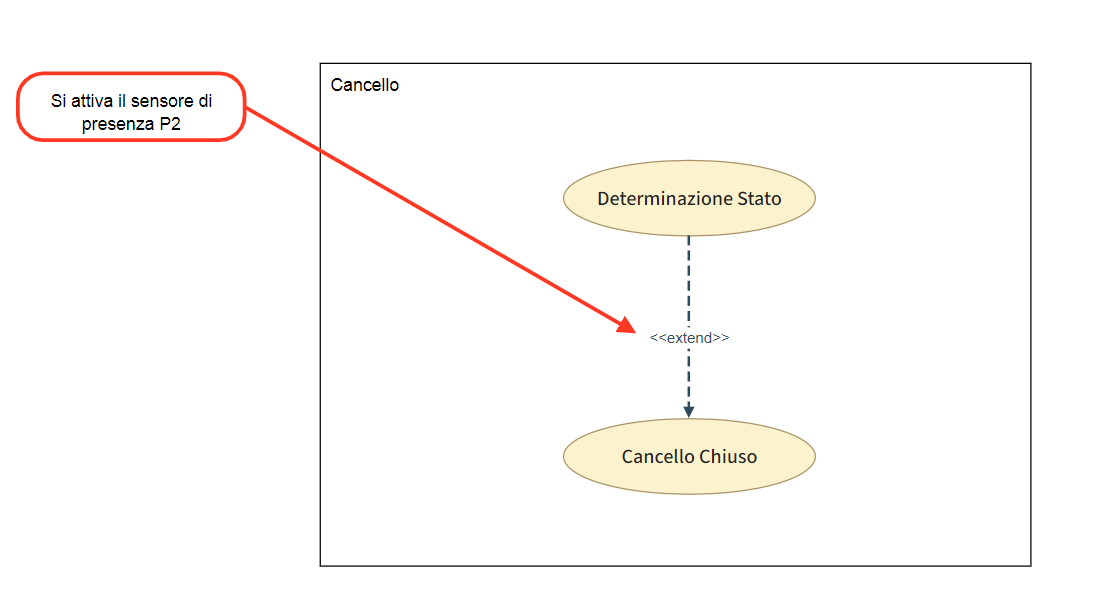
\includegraphics[width=0.9\textwidth]{figures/usecase_7.png}
    \caption{Determinazione Stato}
    \label{usecase7}
\end{figure}


\section{Gestione dello stato di errore [US8-US11]}
L'utente ha la possibilità di richiedere che il dispositivo entri in uno stato di errore nel caso in cui il sensore di presenza P2 non si attivi dopo il tempo di lavoro previsto durante la fase di chiusura del cancello. Questa azione è essenziale per far si che l'utente venga avvisato in caso di malfunzionamento del sensore.
Il dispositivo fornisce un feedback visivo dello stato di errore, dato dall'accensione del LED rosso in caso il cancello non si chiuda entro 10 secondi dal completamento del tempo di lavoro (\ref{usecase8}).

\begin{figure}[H]
    \centering
    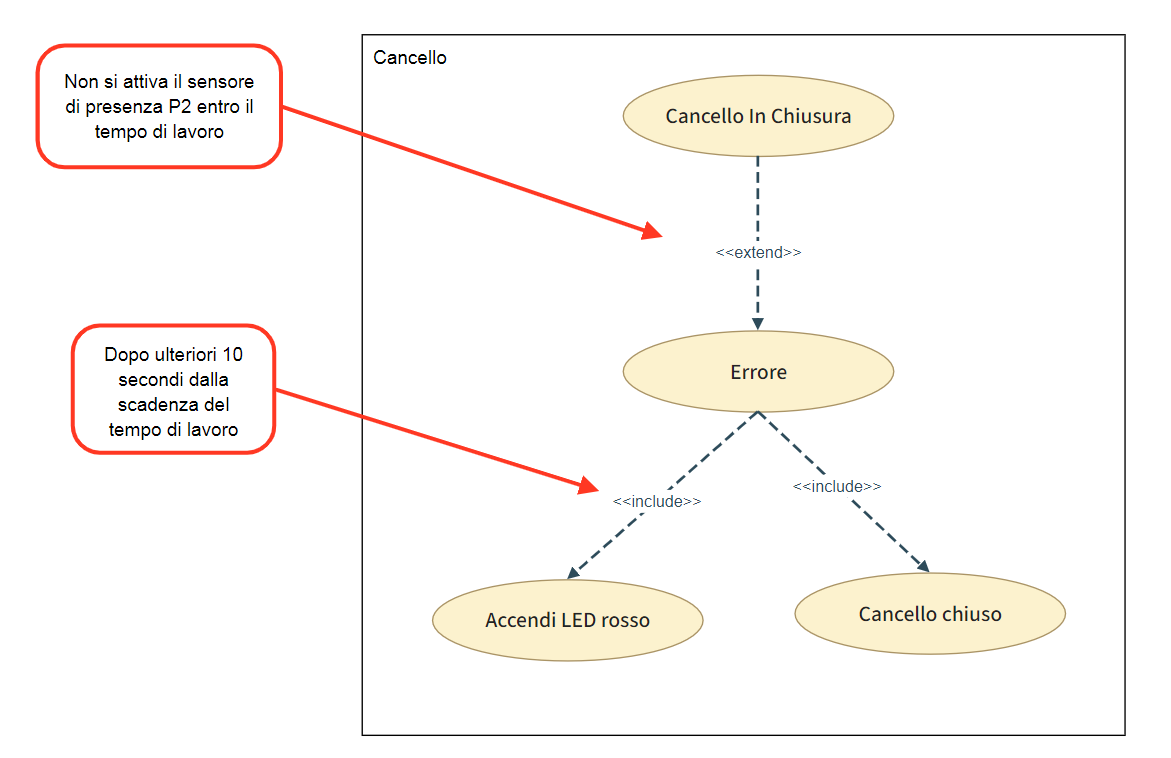
\includegraphics[width=0.9\textwidth]{figures/usecase_8.png}
    \caption{Stato di Errore}
    \label{usecase8}
\end{figure}


\section{Chiusura automatica all'accensione [US9]}
L'utente ha la possibilità di richiedere che il dispositivo avvii la procedura di chiusura del cancello automatico quando il dispositivo viene acceso per la prima volta, solo se i due sensori di presenza P1 e P2 non sono attivi. Questa azione è essenziale per garantire la corretta chiusura del cancello all'accensione del dispositivo.


\begin{figure}[H]
    \centering
    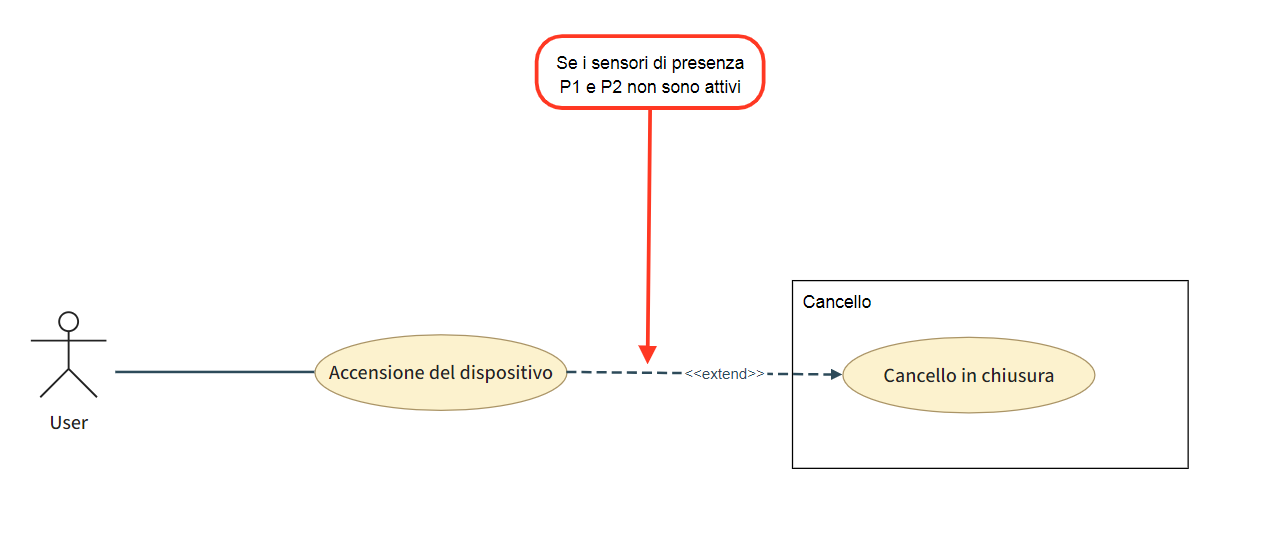
\includegraphics[width=0.9\textwidth]{figures/usecase_9.png}
    \caption{Chiusura Automatica}
    \label{usecase9}
\end{figure}


\section{General Use Case}
\begin{figure}[H]
    \centering
    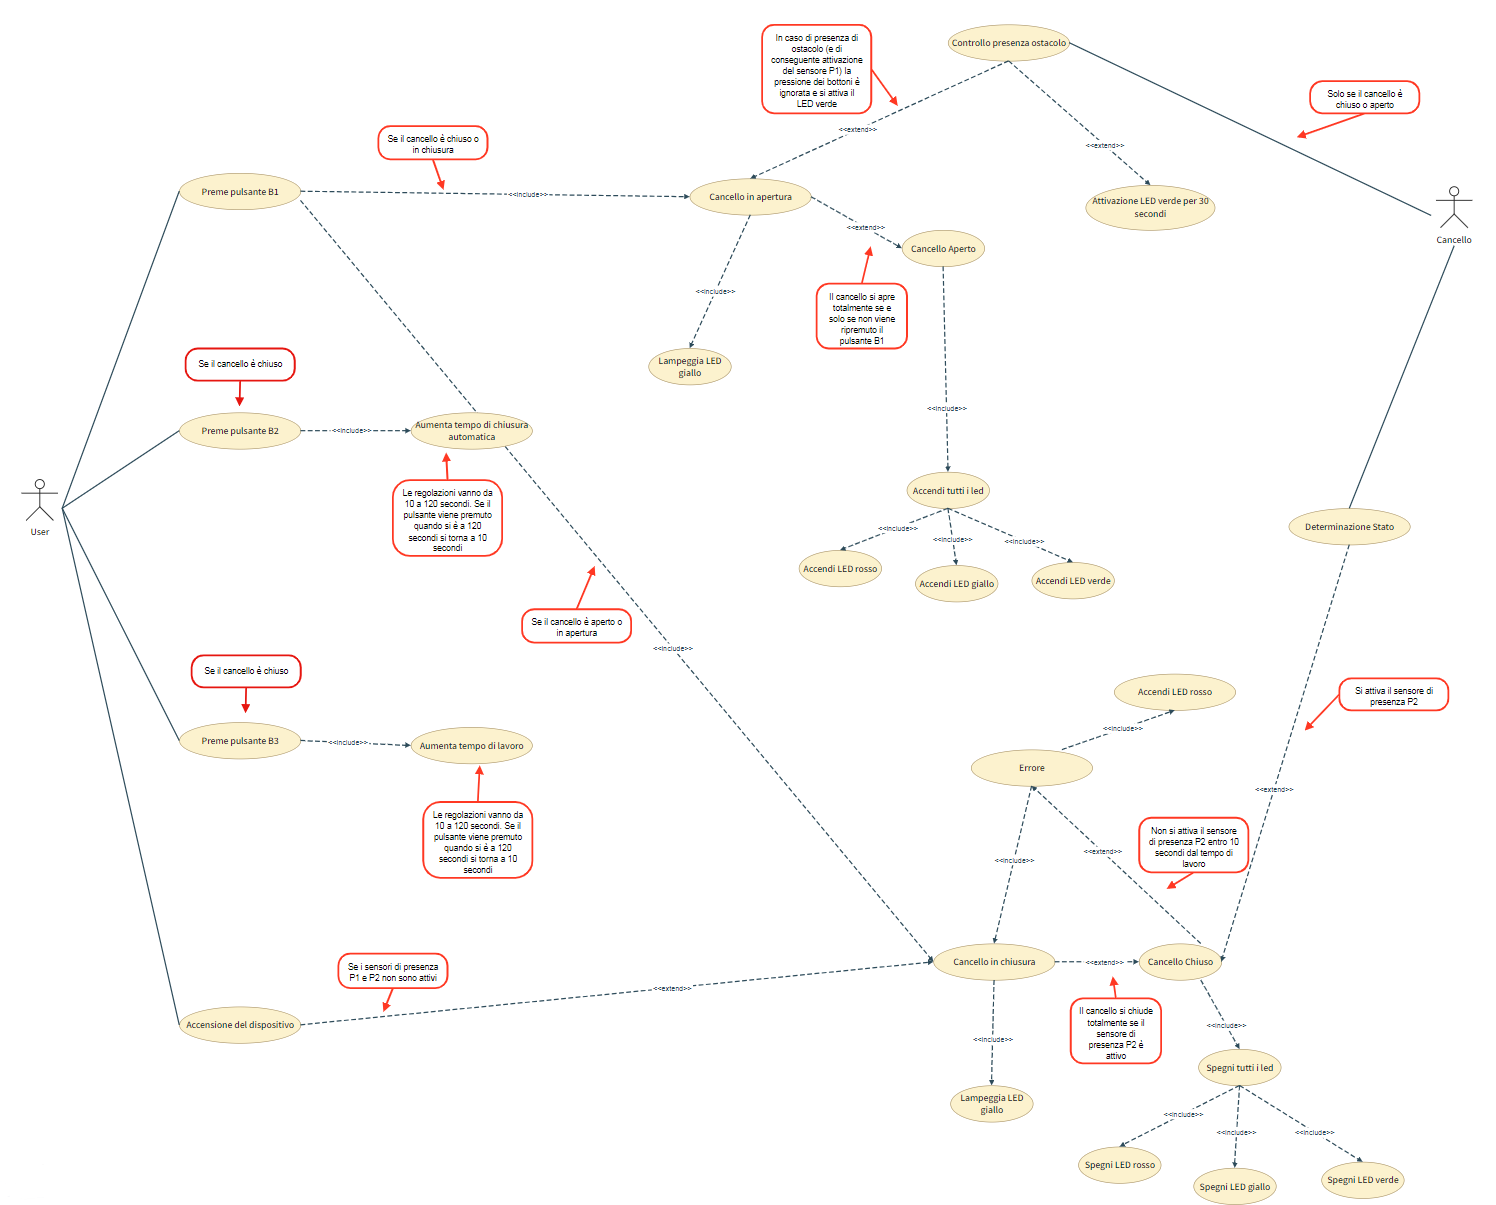
\includegraphics[width=1\linewidth]{figures/generalusecases.png}
    \caption{Use Cases Generale}
    \label{general}
\end{figure}
    \chapter{\bf{Activity Diagrams}}

\section{Apertura e Chiusura Cancello   [Scenario 1]}
Questo scenario, presentato in figura \ref{scenario1}, descrive passo dopo passo le azioni che l’utente compie per aprire e chiudere il cancello, dalle fasi iniziali di richiesta tramite il pulsante B1, fino al feedback visivo che conferma l'operazione completata. Nel seguito verrà presentato il flusso di azioni associato allo scenario corrente:

\noindent Apertura del cancello:
\begin{enumerate}
    \item L’utente decide di aprire il cancello e si avvicina ad esso.
    \item Per avviare il processo di apertura, l’utente preme il pulsante B1.
    \item Il sistema rileva che il pulsante B1 è stato premuto.
    \item Il sistema verifica che il cancello sia chiuso o in chiusura.
    \item Il sistema avvia il processo di apertura del cancello.
    \item Durante l'apertura, il dispositivo fornisce un feedback visivo attivando il lampeggiamento del LED giallo con frequenza 0.5 Hz.
    \item Una volta completata l'apertura, tutti i LED (giallo, rosso e verde) si accendono per indicare la completa apertura del cancello.
\end{enumerate}


\noindent Chiusura del cancello:
\begin{enumerate}
    \item L’utente decide di chiudere il cancello e si avvicina ad esso.
    \item Per avviare il processo di chiusura, l’utente preme il pulsante B1.
    \item Il sistema rileva che il pulsante B1 è stato premuto.
    \item Il sistema verifica che il cancello sia aperto o in apertura.
    \item Il sistema avvia il processo di chiusura del cancello.
    \item Durante la chiusura, il dispositivo fornisce un feedback visivo attivando il lampeggiamento del LED giallo con frequenza 0.5 Hz.
    \item Una volta completata la chiusura, tutti i LED (giallo, rosso e verde) si spengono per indicare la completa chiusura del cancello.
\end{enumerate}


\begin{figure}[H]
    \centering
    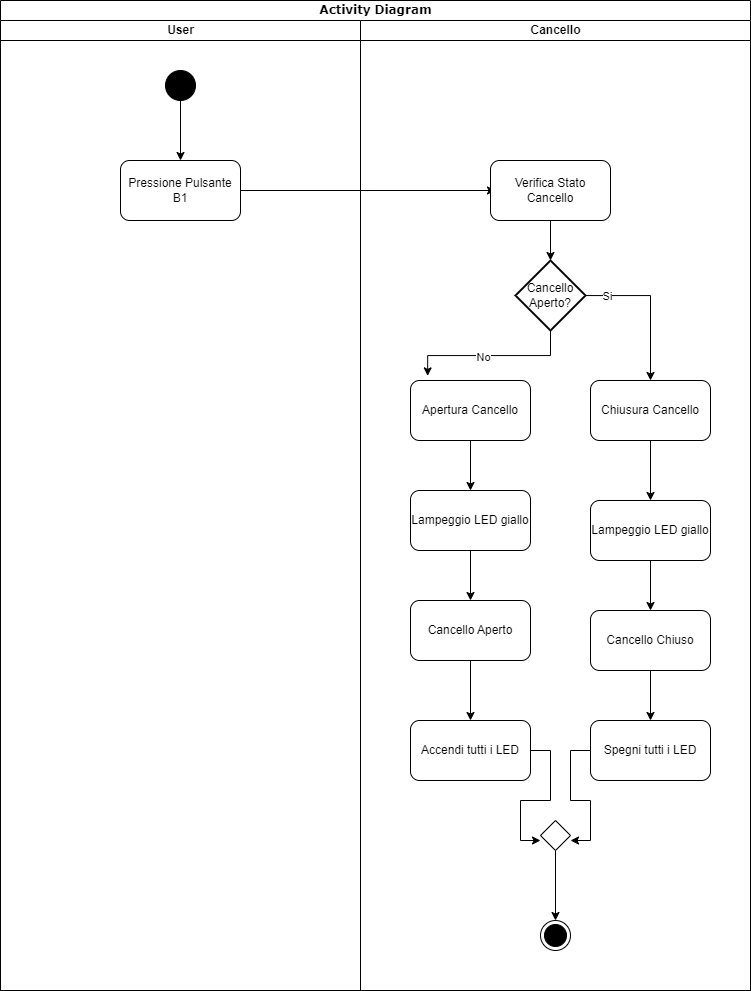
\includegraphics[width=0.9\textwidth]{figures/scenario1.drawio.png}
    \caption{Scenario 1}
    \label{scenario1}
\end{figure}


\section{Regolazioni [Scenario 2]}
Questo scenario, presentato in figura \ref{scenario2}, descrive passo dopo passo le azioni che l’utente compie per regolare il tempo di chiusura automatica del cancello. Nel seguito verrà presentato il flusso di azioni associato allo scenario corrente:

\noindent Regolazione tempo di chiusura automatica:

\begin{enumerate}
\item L’utente decide di regolare il tempo di chiusura automatica del cancello.
\item L’utente si avvicina al cancello chiuso.
\item Per avviare il processo di regolazione, l’utente preme il pulsante B2.
\item Il sistema rileva che il pulsante B2 è stato premuto.
\item Se il tempo di chiusura automatica è inferiore a 120 secondi, ogni pressione del pulsante B2 aumenta il tempo di 10 secondi.
\item Se il tempo di chiusura automatica è già a 120 secondi, premendo nuovamente B2 il tempo viene riportato a 10 secondi.
\end{enumerate}

Questo scenario descrive passo dopo passo le azioni che l’utente compie per regolare la durata delle fasi di apertura e chiusura del cancello. Per questioni di semplicità, il diagramma riguardante quest'attività non è stato riportato poiché identico al precedente.

\noindent Regolazione Tempo di Lavoro:

\begin{enumerate}
\item L’utente decide di regolare la durata delle fasi di apertura e chiusura del cancello.
\item L’utente si avvicina al cancello chiuso.
\item Per avviare il processo di regolazione, l’utente preme il pulsante B3.
\item Il sistema rileva che il pulsante B3 è stato premuto.
\item Ogni pressione del pulsante B3 incrementa la durata di 10 secondi.
\item Se il tempo di lavoro è al massimo (120 secondi), premendo nuovamente B3, il tempo viene riportato a 10 secondi.
\end{enumerate}


\begin{figure}[H]
    \centering
    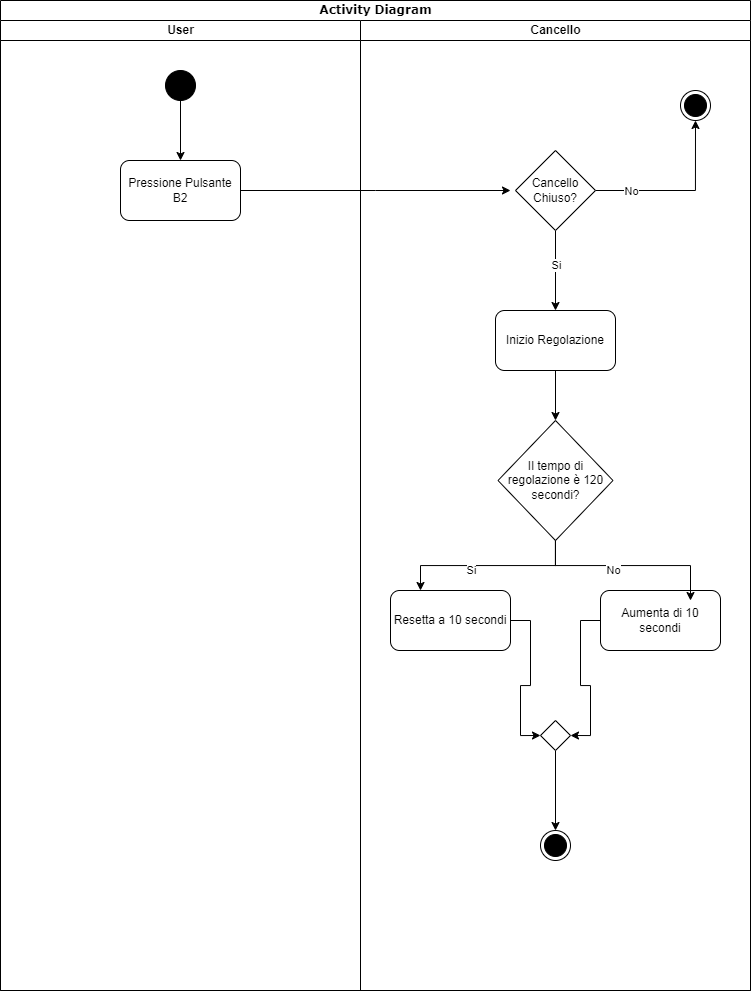
\includegraphics[width=0.9\textwidth]{figures/scenario2.drawio.png}
    \caption{Scenario 2}
    \label{scenario2}
\end{figure}


\section{Gestione Stato e Ostacoli [Scenario 3]}
Questo scenario, presentato in figura \ref{scenario3}, descrive passo dopo passo le azioni che l’utente compie per richiedere la riapertura automatica del cancello in presenza di un ostacolo. Nel seguito verrà presentato il flusso di azioni associato allo scenario corrente:

\noindent Riapertura Automatica con Rilevazione Ostacolo:

\begin{enumerate}
\item Il sistema rileva un ostacolo tramite il sensore di presenza (P1) durante la fase di chiusura del cancello.
\item Il sistema avvia la riapertura automatica del cancello per evitare danni e garantire la sicurezza.
\item Il dispositivo fornisce un feedback visivo in caso di apertura completa del cancello, accendendo tutti i LED (giallo, rosso e verde).
\item Se il sistema non rileva alcun ostacolo procederà con la chiusura del cancello e l'attivazione del sensore di presenza P2.
\end{enumerate}

\noindent Gestione Richieste in presenza di ostacoli:
Questo scenario descrive passo dopo passo le azioni che l’utente compie per gestire le richieste di apertura o chiusura del cancello in presenza di ostacoli. Nel seguito verrà presentato il flusso di azioni associato allo scenario corrente:


\begin{enumerate}
\item L’utente decide di attivare la funzione che fa ignorare le richieste di apertura o chiusura del cancello quando il sensore di presenza (P1) è attivo.
\item Il sistema rileva la presenza di un ostacolo tramite il sensore P1.
\item Il sistema ignora le richieste di apertura o chiusura del cancello per prevenire movimenti non sicuri.
\item Il dispositivo fornisce un feedback visivo della presenza di un ostacolo, facendo lampeggiare il LED verde con una frequenza di 1 Hz per 30 secondi.
\end{enumerate}


\begin{figure}[H]
    \centering
    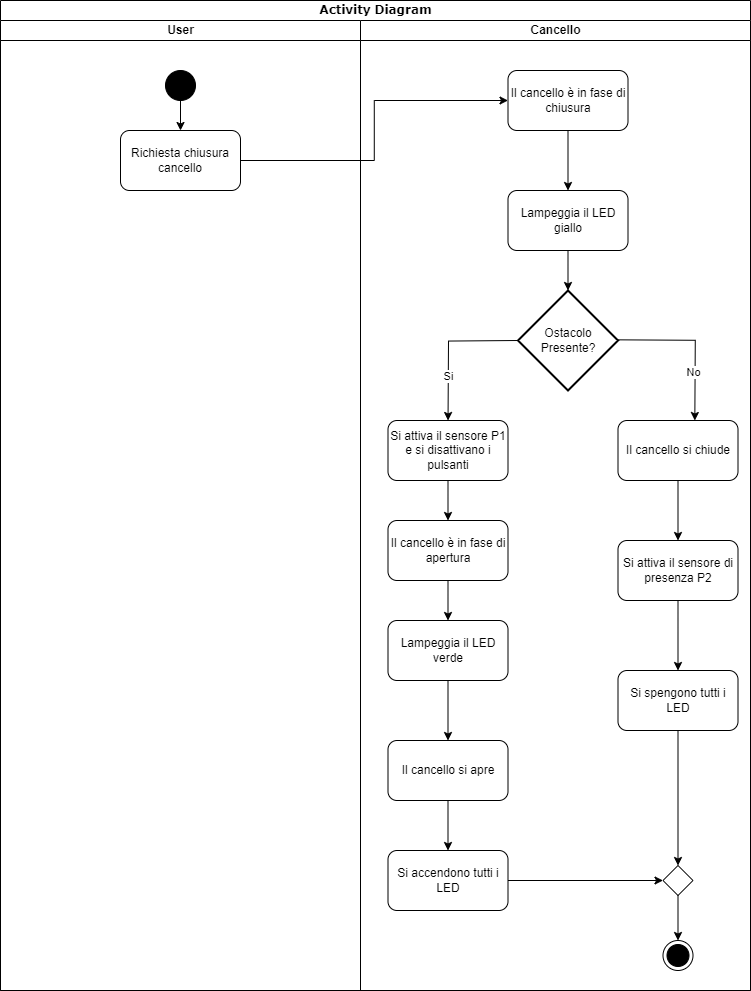
\includegraphics[width=0.9\textwidth]{figures/scenario3.drawio.png}
    \caption{Scenario 3}
    \label{scenario3}
\end{figure}


\section{Stato di Errore [Scenario 4]}
Questo scenario, presentato in figura \ref{scenario4}, descrive passo dopo passo le azioni che l’utente compie per far entrare il dispositivo in uno stato di errore in caso di malfunzionamento del sensore di presenza (P2). Nel seguito verrà presentato il flusso di azioni associato allo scenario corrente:

\noindent Stato di errore con rilevazione malfunzionamento del sensore:

\begin{enumerate}
\item L’utente richiede la chiusura del cancello tramite il pulsante B1
\item Il sistema rileva che il sensore di presenza (P2) non si è attivato dopo il tempo di lavoro previsto durante la fase di chiusura del cancello.
\item Il sistema entra in uno stato di errore per avvisare l’utente del possibile malfunzionamento del sensore.
\item Il dispositivo fornisce un feedback visivo dello stato di errore, accendendo il LED rosso se il cancello non si chiude entro 10 secondi dal completamento del tempo di lavoro.
\end{enumerate}

\begin{figure}[H]
    \centering
    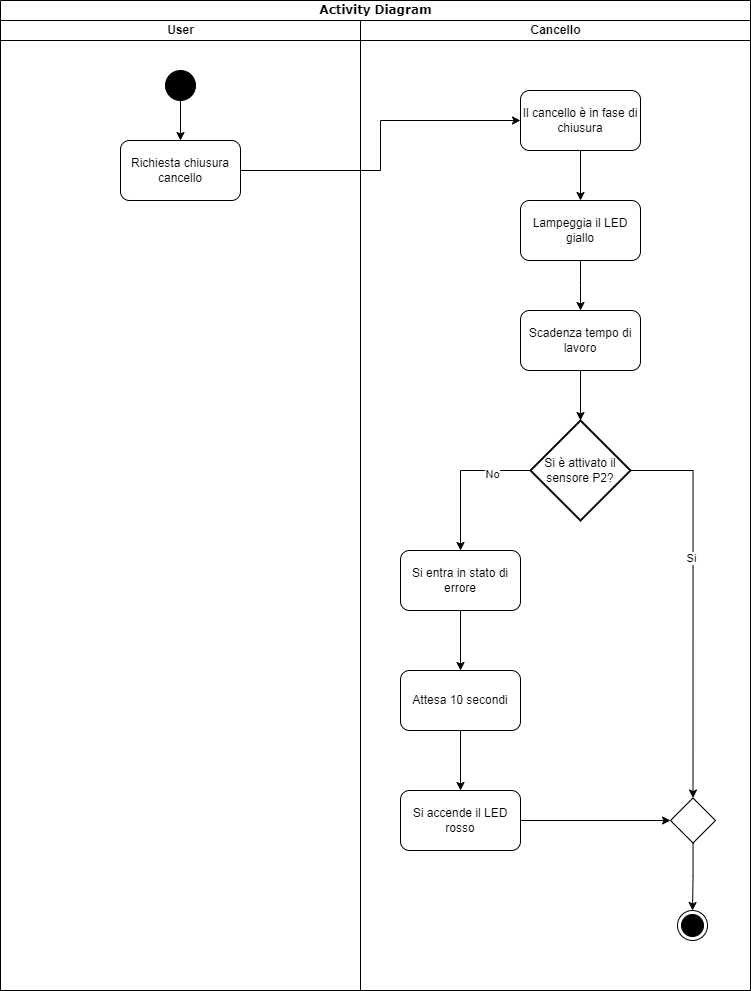
\includegraphics[width=0.9\textwidth]{figures/scenario4.drawio.png}
    \caption{Scenario 4}
    \label{scenario4}
\end{figure}


\section{Chiusura automatica all'accensione [Scenario 5]}
Questo scenario, presentato in Figura 2.7, descrive passo dopo passo le azioni che l’utente compie per richiedere la chiusura automatica del cancello all'accensione del dispositivo. Nel seguito verrà presentato il flusso di azioni associato allo scenario corrente:

\noindent Chiusura automatica all'accensione del dispositivo:

\begin{enumerate}
\item L’utente accende il dispositivo per la prima volta.
\item Il sistema verifica che i sensori di presenza P1 e P2 non siano attivi.
\item Il sistema avvia la procedura di chiusura del cancello.
\item Il dispositivo garantisce la corretta chiusura del cancello all'accensione.
\end{enumerate}


\begin{figure}[H]
    \centering
    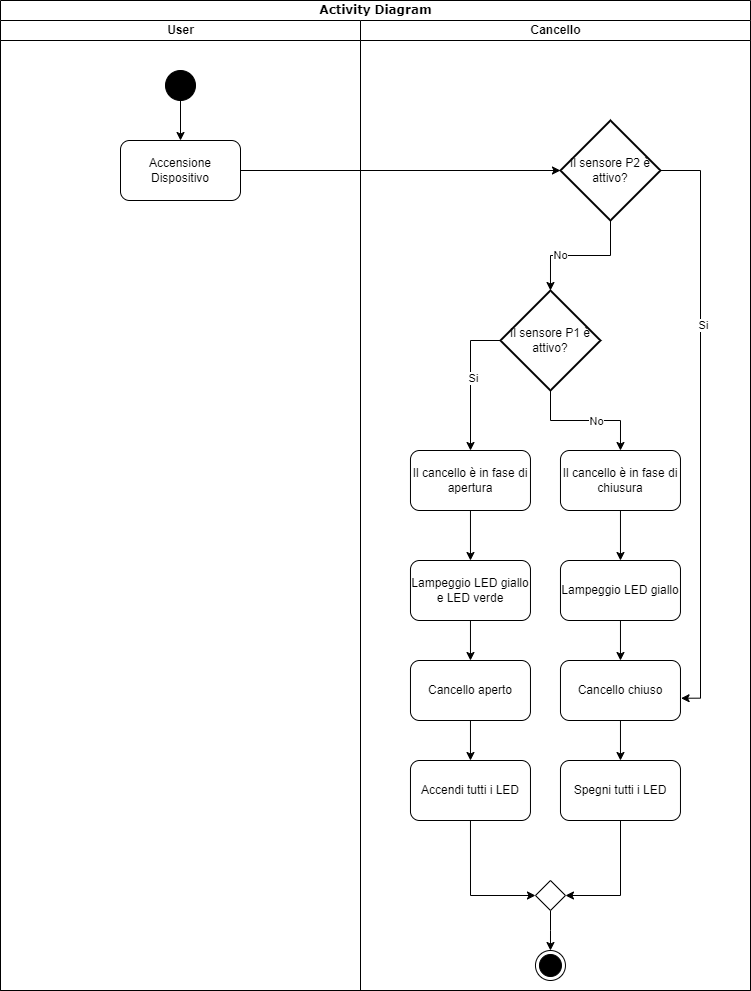
\includegraphics[width=0.9\textwidth]{figures/scenario5.drawio.png}
    \caption{Scenario 5}
    \label{scenario5}
\end{figure}
    \chapter{\bf{State Diagrams}}
    \boldmath

\chapter{Modellazione del Sistema nell'ambiente Simulink}

    \noindent In questo capitolo esploreremo l'ambiente Simulink di MATLAB, uno strumento avanzato per la modellazione, la simulazione e l'analisi di sistemi dinamici. Simulink consente di creare modelli grafici dei sistemi utilizzando un'interfaccia intuitiva a blocchi, facilitando la rappresentazione e la comprensione delle interazioni tra i vari componenti del sistema. Attraverso esempi pratici e casi di studio, illustreremo come costruire modelli accurati, simulare il comportamento del sistema e analizzare i risultati per ottimizzare le prestazioni. Particolare attenzione sarà dedicata a Stateflow, un modulo di Simulink specializzato nella gestione di logiche basate su stati, condizioni decisionali e comportamenti che cambiano nel tempo.

    \section{Gate Chart}
        In questa sezione esamineremo l'implementazione del modulo principale \textbf{Cancello}, che si occupa della movimentazione dello stesso, dell'attivazione e disattivazione dei LED, e della gestione dello stato di errore.

        \newpage
            
        \subsection{Variabili}
            Le variabili presenti all'interno del macrostato sono le seguenti:
            \begin{table}[H]
                \centering
                    \begin{tabular}{ | c | c | c | c |} 
                        \hline
                        \textbf{Tipo} & \textbf{Nome} & \textbf{Valore} & \textbf{Descrizione} \\
                        
                        \hline
                        local\_data & Var\_Inattivo & ON/OFF &  \makecell{Variabile utilizzata per segnalare \\ che lo stato Inattivo è attualmente attivo}\\
                        
                        \hline
                        local\_data & Var\_Chiuso & ON/OFF & \makecell{Variabile utilizzata per segnalare \\ che lo stato Chiuso è attualmente attivo} \\
                        
                        \hline
                        local\_data & Var\_Aperto & ON/OFF & \makecell{Variabile utilizzata per segnalare \\ che lo stato Aperto è attualmente attivo} \\
                        
                        \hline
                        local\_data & Var\_In\_Chiusura & ON/OFF & \makecell{Variabile utilizzata per segnalare \\ che lo stato In Chiusura è attualmente attivo} \\
                        
                        \hline
                        output\_data & LedG & ON/OFF & \makecell{Variabile utilizzata per l'attivazione del \\ LED verde in output} \\
                        
                        \hline
                        output\_data & LedR & ON/OFF & \makecell{Variabile utilizzata per l'attivazione del \\ LED Rosso in output} \\
                        
                        \hline
                        output\_data & LedY & ON/OFF & \makecell{Variabile utilizzata per l'attivazione del \\ LED Giallo in output} \\
                        
                        \hline
                        input\_data & P1 & ON/OFF & \makecell{Variabile utilizzata per \\ la segnalazione di un ostacolo} \\
                        
                        \hline
                        input\_data & P2 &ON/OFF & \makecell{Variabile utilizzata per \\ la segnalazione della chiusura del cancello} \\
                        
                        \hline
                        constant\_data & Blink\_Period & 2 & \makecell{Costante utilizzata per la durata del \\ blink del LED Giallo} \\
                        
                        \hline
                        local\_data & $T_L$ & [10, 120] & Contatore del tempo di lavoro \\
                        
                        \hline
                        local\_data & $T_C$ & [10, 120] & Contatore del tempo di chiusura \\
                        
                        \hline
                        constant\_data & ErrDur & 10 & \makecell{Costante utilizzata per la durata del \\ lampeggio del LED rosso} \\
                        
                        \hline
                        local\_event & buttonpressed1 & TRUE/FALSE & Evento per la pressione del pulsante B1 \\
                        
                        \hline
                    \end{tabular}
                \caption{Tabella variabili Cancello}
            \end{table}

        \subsection{Stati e Funzionamento}
            Il macrostato \textbf{Cancello} presenta i seguenti stati e macrostati:
                
            \begin{itemize}
                \item \textbf{Inattivo}
                    
                \item \textbf{Chiusura}  
                    \begin{itemize}    
                        \item In Chiusura  
                            \begin{itemize}
                                \item Blink\_COff
                                    
                                \item Blink\_COn
                            \end{itemize}
                        
                        \item Chiuso
                        
                        \item Errore
                            \begin{itemize}
                                \item In errore
                                    
                                    \begin{itemize}
                                        \item Blink\_EOff
                                            
                                        \item Blink\_EOn
                                    \end{itemize}
                                
                                \item Led\_Rosso\_Errore
                            \end{itemize}
                    \end{itemize}
                    
                \item \textbf{Apertura}
                    \begin{itemize}
                        \item In Apertura
                            \begin{itemize}
                                \item Blink\_AOff
                                    
                                \item Blink\_AOn 
                            \end{itemize}
                            
                        \item Aperto
                            
                        \item Aperto\_Con\_Ostacolo
                    \end{itemize}
            \end{itemize}
                
            \begin{figure}[H]
                \centering
                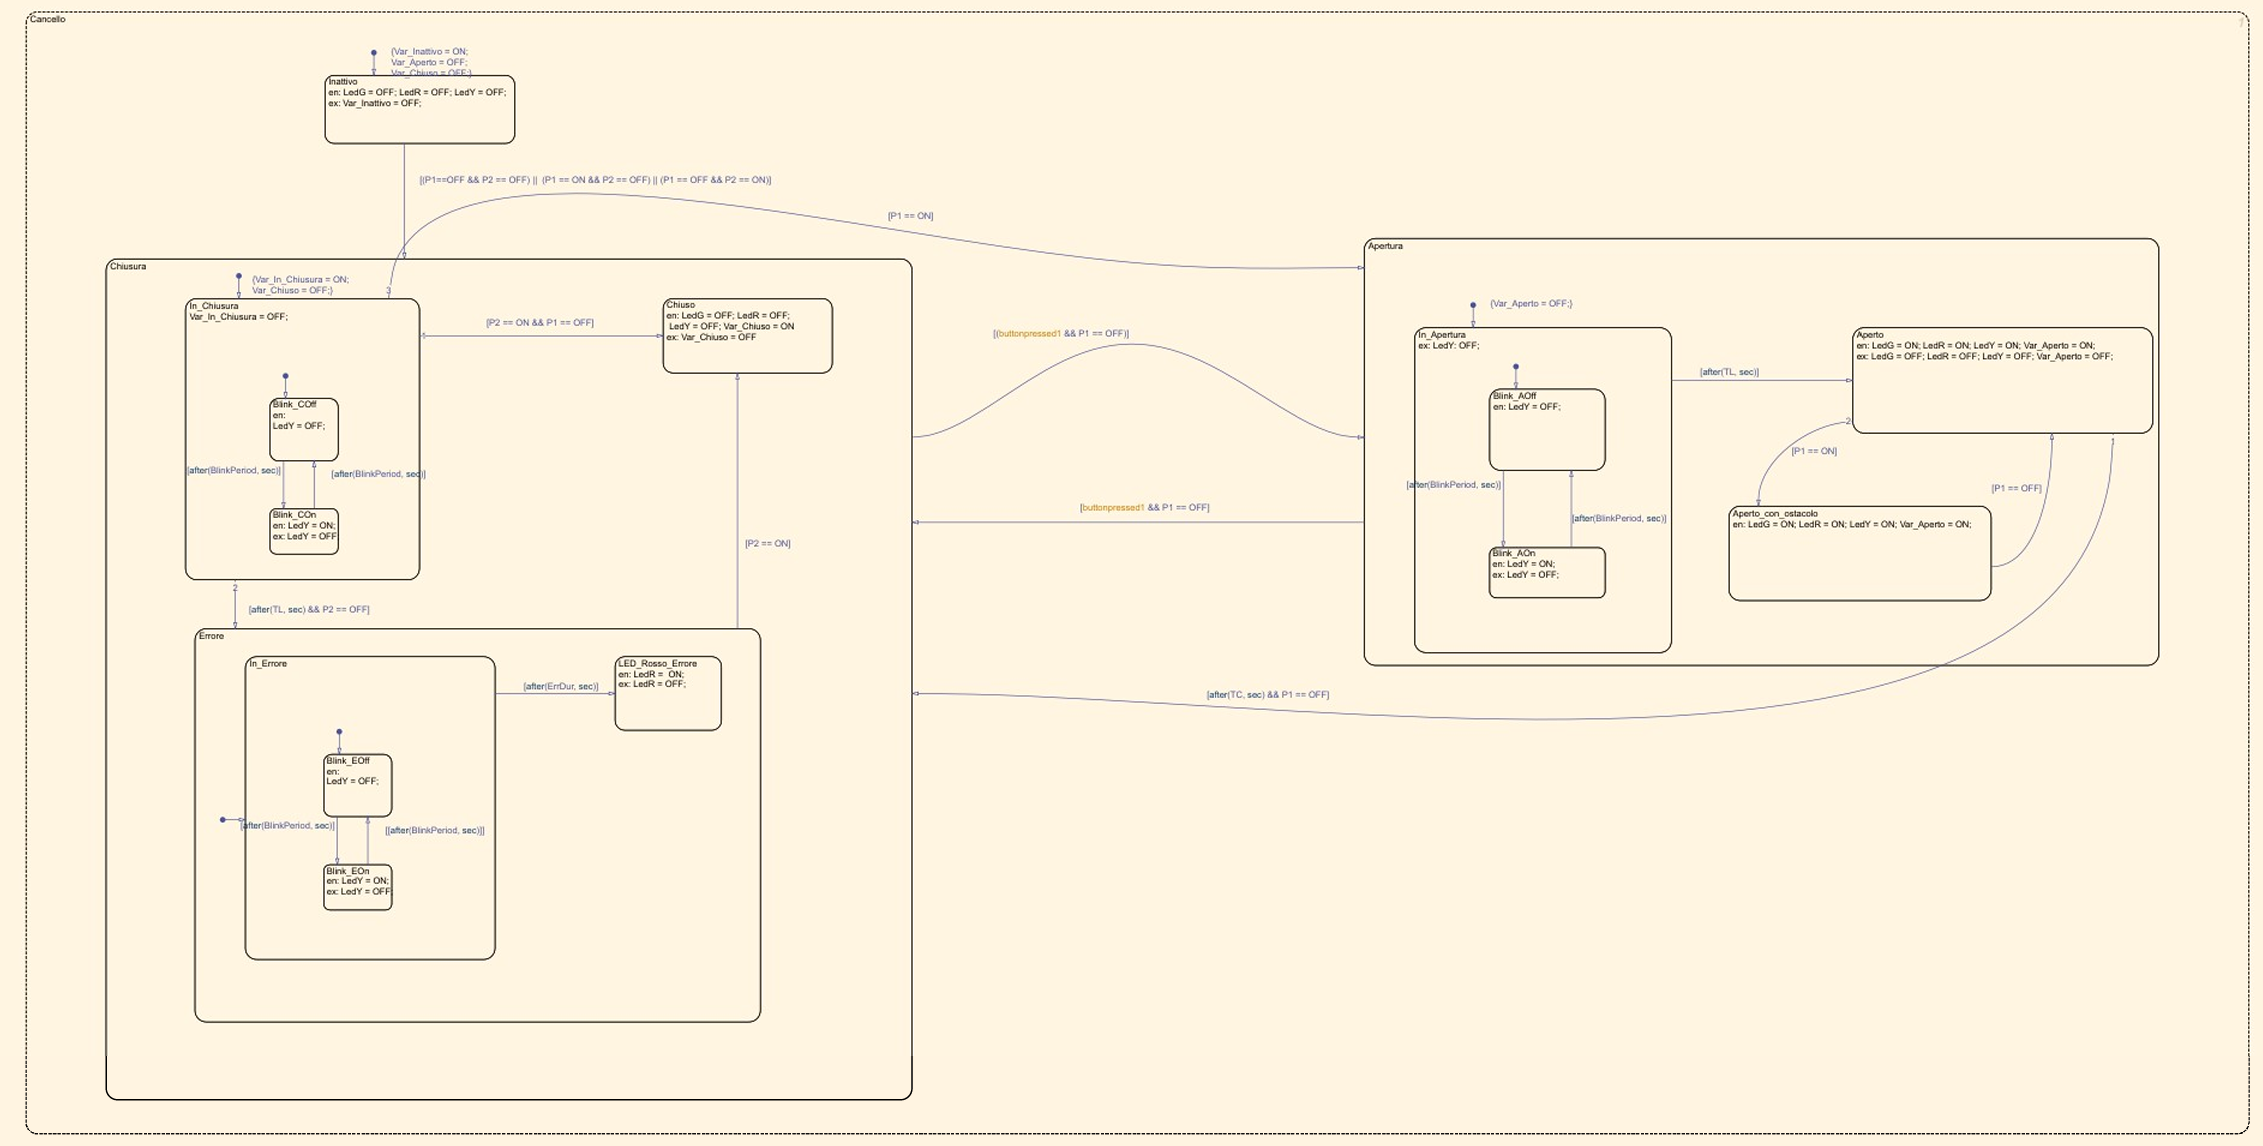
\includegraphics[width=0.9\textwidth]{figures/gate.png}
                \caption{Stato Cancello}
                \label{gate}
            \end{figure}

            \noindent Proseguiamo ora descrivendo il funzionamento dell'intero macrostato \textbf{Cancello}
        
            \begin{enumerate}
                \item All'avvio del sistema lo stato è impostato come \textbf{Inattivo}, inizializza le tre variabili \textit{Var\_Inattivo}, \textit{Var\_Aperto} e \textit{Var\_Chiuso} e si occupa di spegnere tutti i LED.
                Quando si esce da codesto stato, si pone \textit{Var\_Inattivo} ad OFF.
                La condizione di uscita prevede che si vada nello stato \textbf{Chiusura} se e solo se i due sensori di presenza non sono contemporaneamente e inizialmente attivi.
                
                \item All'interno del macrostato \textbf{Chiusura}, lo stato iniziale è \textbf{In\_Chiusura}, in cui viene inizializzata la variabile \textit{Var\_In\_Chiusura} ad ON, mentre la variabile \textit{Var\_Chiuso} viene posta ad OFF.
                Inoltre, nel macrostato \textbf{In\_Chiusura}, avviene il blink del LED giallo grazie all'alternarsi degli stati sottostanti con periodo di 2 secondi. \\
                Le transizioni in uscita da questo stato sono:
            
                \begin{itemize}
                    \item Se si attiva il sensore di presenza P2 di chiusura del cancello, ed il sensore P1 risulta spento (non rilevando dunque ostacoli), si entra nello stato \textbf{Chiuso}, nel quale vengono spenti tutti i LED e viene attivata la variabile \textit{Var\_Chiuso}
                    
                    \item Se scade il timer riguardante il tempo di lavoro \textbf{$T_L$} senza conseguente attivazione del sensore di presenza P2, si entra nello stato \textbf{Errore}, nel quale si accende il LED rosso se e solo se vi si permane  per ulteriori 10 secondi. Si esce da questo stato solo se ritorna attivo il sensore di presenza P2
                    
                    \item Se invece, si attiva il sensore di presenza P1 che rileva un ostacolo durante la chiusura, si entra nel macrostato \textbf{Apertura}
                \end{itemize}
            
                \item All'interno del macrostato \textbf{Apertura}, lo stato iniziale è quello \textbf{In\_Apertura}, nel quale viene effettuato il blink del LED giallo grazie all'alternarsi degli stati sottostanti con periodo di 2 secondi.
                Da questo stato si esce solo quando scade il tempo di lavoro \textbf{$T_L$} per poi passare allo stato \textbf{Aperto}.
                
                \item In questo stato vengono accesi tutti i LED per segnalare la corretta apertura del cancello e viene posta ad ON la variabile \textit{Var\_Aperto}. In uscita da questo stato invece, i LED verranno spenti ponendo ad OFF la variabile \textit{Var\_Aperto}. \\
                Le possibili transizioni per uscire da questo stato sono:
                
                \begin{itemize}
                    \item Se viene rilevato un ostacolo si entra nello stato \textbf{Aperto\_Con\_Ostacolo} nel quale vengono riaccesi tutti i LED e l'unica transizione possibile per uscire da questo stato è quando non viene più rilevato.
                    Questa funzionalità è stata implementata per azzerare il timer di chiusura ogni volta che un ostacolo viene rilevato
                    
                    \item Se scade il tempo di chiusura e non viene rilevato alcun ostacolo, allora si entra nel macrostato \textbf{Chiusura}, il quale avvia il processo di chiusura del cancello
                \end{itemize}
                
                \item Sia nel macrostato \textbf{Chiusura} che \textbf{Apertura}, la transizione di uscita è identica, nella quale viene premuto il pulsante B1 e non vi sono ostacoli rilevati dal sensore di presenza P1.
            \end{enumerate}


    \section{Tuning Charts}
        In questa sezione analizzeremo l'implementazione dei due moduli utilizzati per le regolazioni, \textbf{Regolazione\_Tempo\_Chiusura} e \textbf{Regolazione\_Tempo\_Lavoro}.
        Essi permettono di regolare le due variabili \textbf{$T_C$} e \textbf{$T_L$} attraverso la pressione dei pulsanti \textbf{$B2$} e \textbf{$B3$} rispettivamente.

        \subsection{Variabili}
            Le variabili presenti all'interno dei due macrostati sono le seguenti:
            
            \begin{table}[H]
                \centering
                    \begin{tabular}{ | c | c | c | c |} 
                        \hline
                        
                        \textbf{Tipo} & \textbf{Nome} & \textbf{Valore} & \textbf{Descrizione} \\ 
                        \hline
                        
                        input\_data & $T_L$ & [10, 120] & Contatore del tempo di lavoro \\ 
                        \hline
                        
                        input\_data & Var\_Chiuso & ON/OFF & \makecell{Variabile utilizzata per segnalare \\ che lo stato Chiuso è attualmente attivo} \\ 
                        \hline
                        
                        local\_event & buttonpressed3 & TRUE/FALSE & Evento per la pressione del pulsante B3 \\ 
                        \hline
                        
                        input\_data & $T_C$ & [10, 120] & Contatore del tempo di chiusura \\ 
                        \hline
                        
                        local\_event & buttonpressed2 & TRUE/FALSE & Evento per la pressione del pulsante B2 \\ 
                        \hline
                    \end{tabular}
                \caption{Tabella variabili Tuning}
            \end{table}

        \subsection{Stati e Funzionamento}
            \noindent I due macrostati presentano i seguenti stati al loro interno:
            
            \begin{itemize}
                \item \textbf{Regolazione\_Tempo\_Lavoro}
                \begin{itemize}
                    \item \textit{Tempo\_Lavoro}
                    \item \textit{Aggiunta\_Tempo\_Lavoro}
                \end{itemize}

                \item \textbf{Regolazione\_Tempo\_Lavoro}
                \begin{itemize}
                    \item \textit{Tempo\_Chiusura}
                    \item \textit{Aggiunta\_Tempo\_Chiusura}
                \end{itemize}
            \end{itemize}

            \begin{figure}[H]
                \centering
                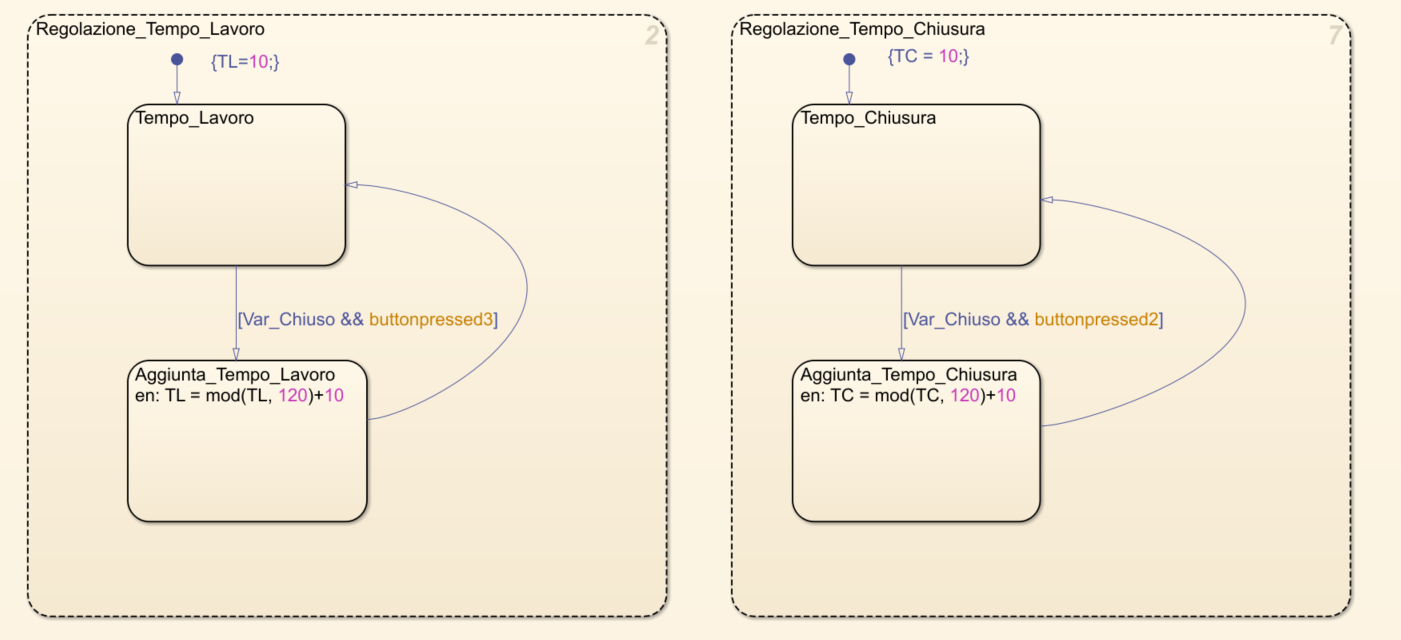
\includegraphics[width=0.9\textwidth]{figures/tuning.png}
                \caption{Stati Regolazioni}
                \label{tuning}
            \end{figure}

            \noindent Proseguiamo ora analizzando il funzionamento di un singolo macrostato \textbf{(Regolazione\_Tempo\_Chiusura)}, essendo l'altro identico per costruzione:

            \begin{enumerate}
                \item Si parte dallo stato \textbf{Tempo\_Chiusura} nel quale la variabile \textbf{$T_C$} viene inizializzata al valore 10 (secondi).
                
                \item In seguito, se ci troviamo nello stato \textbf{Chiuso} e parallelamente viene rilevata la pressione del pulsante \textbf{B2} allora, ci spostiamo nello stato \textbf{Aggiunta\_Tempo\_Chiusura} nel quale la variabile $T_C$ viene incrementata di 10 (secondi).
                
                \item Una volta avvenuto l'incremento, si ritorna nello stato iniziale \textbf{Tempo\_Chiusura} nel quale si resta in attesa delle condizioni tali per cui si possono effettuare gli ulteriori incrementi.
            \end{enumerate}


    \section{Obstacle Chart}
        In questa sezione analizzeremo l'implementazione del macrostato \textbf{Ostacolo}, il quale consente la gestione del sistema in caso di rilevazione dello stesso. Esso permette il lampeggio del LED verde in output, nel caso il sensore di presenza \textbf{P1} si attivi.

        \subsection{Variabili}
            Le variabili all'interno del macrostato sono le seguenti:
            
            \begin{table}[H]
                \centering
                    \begin{tabular}{ | c | c | c | c |} 
                        \hline
                        
                        \textbf{Tipo} & \textbf{Nome} & \textbf{Valore} & \textbf{Descrizione} \\ 
                        \hline
                        
                        constant\_data & GreenDur & 30 & \makecell{Costante utilizzata per la durata del \\ lampeggio del LED verde} \\ 
                        \hline
                        
                        input\_data & Var\_Chiuso & ON/OFF & \makecell{Variabile utilizzata per segnalare \\ che lo stato Chiuso è attualmente attivo} \\ 
                        \hline
                        
                        input\_data & Var\_Inattivo & ON/OFF & \makecell{Variabile utilizzata per segnalare \\ che lo stato Inattivo è attualmente attivo} \\ 
                        \hline
                        
                        input\_data & Var\_Aperto & ON/OFF & \makecell{Variabile utilizzata per segnalare \\ che lo stato Aperto è attualmente attivo} \\ 
                        \hline
                        
                        local\_event & buttonpressed1 & TRUE/FALSE & Evento per la pressione del pulsante B1 \\ 
                        \hline
                        
                        constant\_data & BlinkPeriod2 & 1 & \makecell{Costante utilizzata per la durata del \\ blink del LED verde} \\ 
                        \hline
                        
                        input\_data & P1 & ON/OFF & \makecell{Variabile utilizzata per \\ la segnalazione di un ostacolo} \\ 
                        \hline
                        
                        output\_data & LedG & ON/OFF & \makecell{Variabile utilizzata per l'attivazione del \\ LED verde in output} \\ 
                        \hline
                    \end{tabular}
                \caption{Tabella variabili Ostacolo}
            \end{table}

        \subsection{Stati e Funzionamento}
            Il macrostato \textbf{Ostacolo} presenta i seguenti stati al suo interno:
            
            \begin{itemize}
                \item \textbf{Fermo}
                
                \item \textbf{Ostacolo\_Presente}
                
                \item \textbf{Blink\_OOff}
                
                \item \textbf{Blink\_OOn}
                
                \item \textbf{Aperto\_Con\_Ostacolo\_Led}
            \end{itemize}

            \begin{figure}[H]
                \centering
                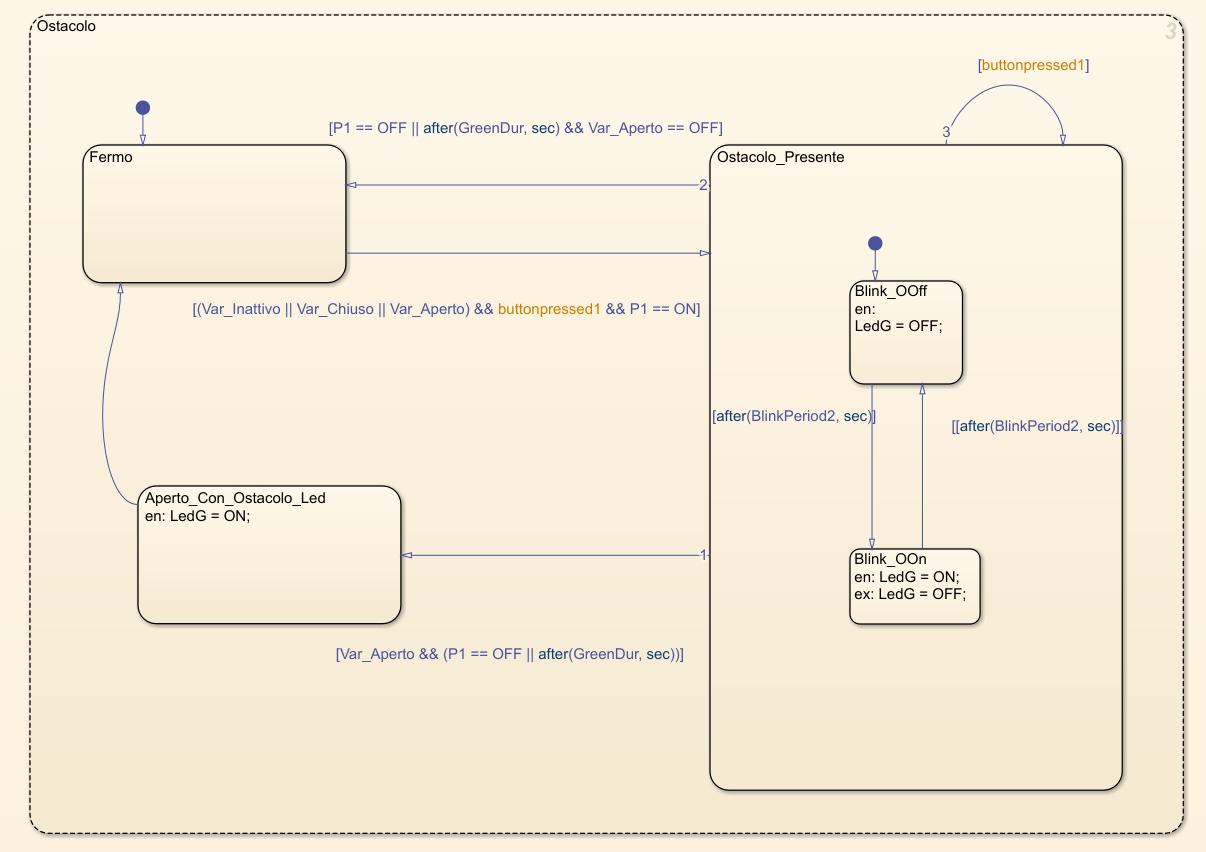
\includegraphics[width=0.9\textwidth]{figures/obstacle.png}
                \caption{Stato Ostacolo}
                \label{obstacle}
            \end{figure}

            \noindent Proseguiamo ora descrivendo il funzionamento dell'intero macrostato \textbf{Ostacolo}:
            
            \begin{enumerate}
                \item All'attivazione del sistema, si entra nello stato \textbf{Fermo} (che rappresenta uno stato di \textit{Idle}) dal quale si esce solo quando ci si trova  o nello stato \textbf{Inattivo} o nello stato \textbf{Chiuso} o nello stato \textbf{Aperto} e al contempo il sensore di presenza \textbf{P1} è attivo con annessa rilevazione di pressione del pulsante \textbf{$B1$}.
                
                \item La transizione sopra citata, ci porta nello stato \textbf{Ostacolo\_Presente} nel quale viene effettuato il \textit{blink} del LED verde.
                Nel dettaglio, lo stato iniziale del blink è \textbf{Blink\_OOff} il quale si occupa di spegnere il LED verde, mentre lo stato \textbf{Blink\_OOn} si occupa di accenderlo.
                La transizione tra i due stati avviene in accordo alla scadenza di un timer, di durata pari a \textbf{Blink\_Period2}, ovvero 1 secondo.
                
                \item Dall'attuale stato, si esce quando si verifica una delle seguenti condizioni:
                
                    \begin{itemize}
                        \item Non viene più rilevato l'ostacolo poiché il sensore di presenza P1 si disattiva, oppure poiché scade il timer associato al lampeggio del LED.
                        In aggiunta a questi requisiti \textbf{Var\_Aperto} deve essere uguale ad OFF.
                        In questo caso, ritorniamo nello stato \textbf{Fermo}.
                        
                        \item Non viene più rilevato l'ostacolo poiché il sensore di presenza P1 si disattiva, oppure poiché scade il timer associato al lampeggio del LED, ma ci troviamo parallelamente nello stato \textbf{Aperto}, dunque, il nuovo stato diventa \textbf{Aperto\_Con\_Ostacolo\_Led} nel quale viene riattivato il LED verde dopo il lampeggio.
                        Infine si ritorna nello stato \textbf{Fermo}.
                        \item Si preme il pulsante B1 e si ritorna nello stato \textbf{Ostacolo\_Presente} in modo da resettare il timer di 30 secondi relativo al lampeggio del LED verde.
                    \end{itemize}
            \end{enumerate}


    \section{Buttons Charts}
        In questa sezione analizzeremo l'implementazione dei macrostati \textbf{Button}. Essi permettono di rilevare quando il pulsante è stato premuto consentendo l'attivazione dell'evento. 
        Vedremo prima l'implementazione del macrostato \textbf{Button1} e successivamente di \textbf{Button2} e \textbf{Button3} che sono identici per costruzione.

        \subsection{Variabili}
        Le variabili all'interno del macrostato \textbf{Button1} sono le seguenti:

            \begin{table}[H]
                \centering
                    \begin{tabular}{ | c | c | c | c |} 
                        \hline
                        \textbf{Tipo} & \textbf{Nome} & \textbf{Valore} & \textbf{Descrizione} \\ 
                        
                        \hline
                        input\_data & B1 & ON/OFF & \makecell{Variabile utilizzata per segnalare \\ la pressione del pulsante} \\ 
                        
                        \hline
                        local\_event & buttonpressed1 & TRUE/FALSE & Evento per la pressione del pulsante B1 \\ 
                        
                        \hline
                    \end{tabular}
                \caption{Tabella variabili Button1}
            \end{table}
            
            Le variabili all'interno dei macrostati \textbf{Button2} e \textbf{Button3} sono le seguenti:

            \begin{table}[H]
                \centering
                    \begin{tabular}{ | c | c | c | c |} 
                        \hline
                        \textbf{Tipo} & \textbf{Nome} & \textbf{Valore} & \textbf{Descrizione} \\ 
                        \hline
                        input\_data & B2 & ON/OFF & \makecell{Variabile utilizzata per segnalare \\ la pressione del pulsante} \\ 
                        \hline
                        local\_event & buttonpressed2 & TRUE/FALSE & Evento per la pressione del pulsante B2 \\ 
                        \hline
                        input\_data & B3 & ON/OFF & \makecell{Variabile utilizzata per segnalare \\ la pressione del pulsante} \\ 
                        \hline
                        local\_event & buttonpressed3 & TRUE/FALSE & Evento per la pressione del pulsante B3 \\ 
                        \hline
                    \end{tabular}
                \caption{Tabella variabili Button2 e Button3}
            \end{table}

        \subsection{Stati e Funzionamento}
            Proseguiamo ora descrivendo inizialmente il funzionamento del macrostato \textbf{Button1} e successivamente dei restanti. Tutti i pulsanti  presentano un'implementazione su fronte di discesa.

            \begin{figure}[H]
                \centering
                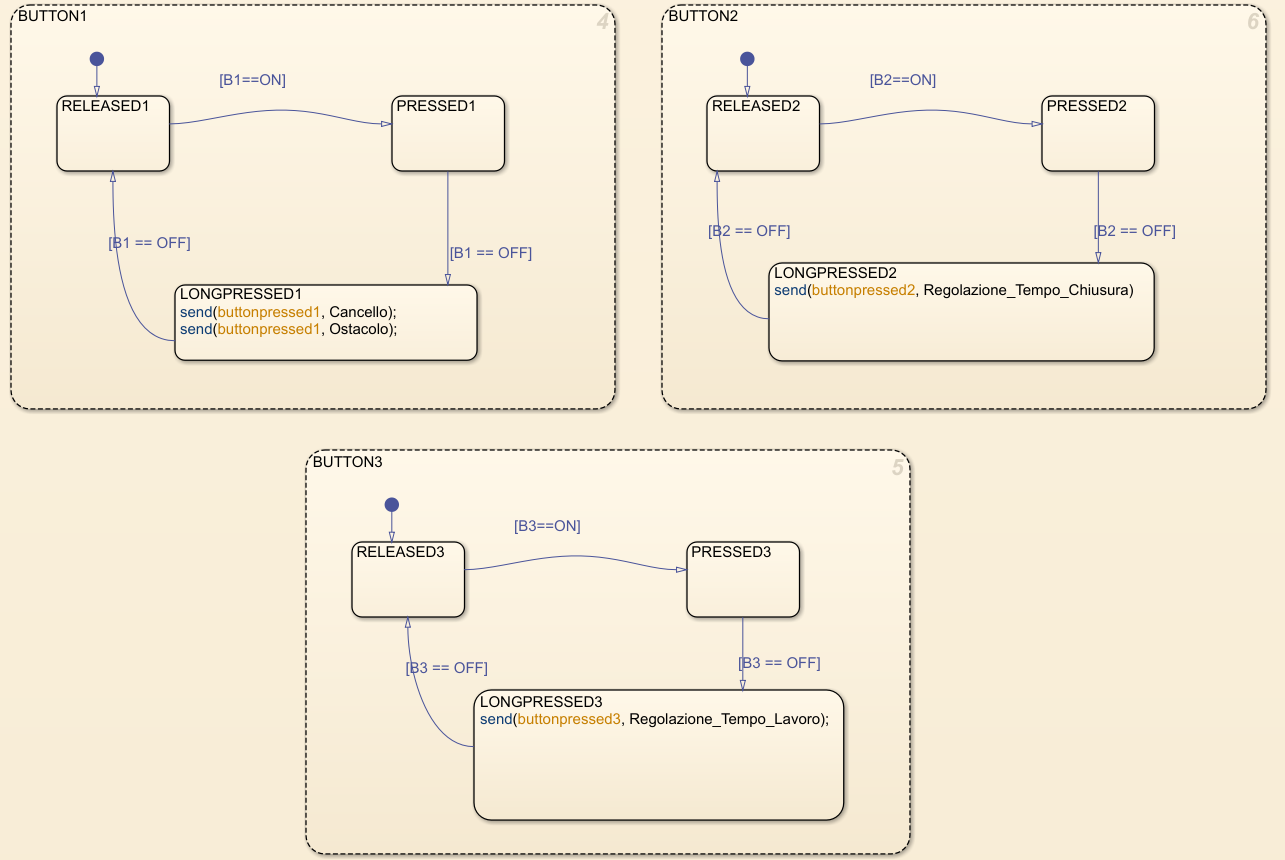
\includegraphics[width=0.9\textwidth]{figures/buttons.png}
                \caption{Stati Buttons}
                \label{buttons}
            \end{figure}

            \noindent \textbf{Button1:}
            \begin{enumerate}
                \item Si entra nello stato \textbf{Released1}, il quale sottolinea il fatto che all'accensione del sistema il pulsante è rilasciato.
                
                \item Alla pressione del pulsante B1 si entra nello stato \textbf{Pressed1}, per segnalare che il pulsante è stato premuto. Questi due stati non presentano azioni in entrata o in uscita, ma sono utilizzati solo per rappresentare l'interazione con l'utente.
                
                \item Quando verrà rilasciato il pulsante, ovvero quando B1 == OFF, si entra nello stato \textbf{Longpressed1}, il quale si occupa di inviare l'evento \textit{buttonpressed1} ai due macrostati \textbf{Cancello} e \textbf{Ostacolo} per segnalare la corretta pressione del pulsante. 
            \end{enumerate}

            \noindent \textbf{Button2 e Button3:}

            \begin{enumerate}
                \item Si entra nello stato \textbf{Released2/Released3}, il quale sottolinea che all'accensione del sistema il pulsante viene rilasciato.
                
                \item Alla pressione del pulsante B2/B3 si entra nello stato \textbf{Pressed2/Pressed3}, per indicare che il pulsante è stato premuto. Questi due stati non posseggono azioni in entrata o in uscita, ma segnalano solo l'interazione con l'utente.
                
                \item Quando verrà rilasciato il pulsante, ovvero quando B2/B3 == OFF, si entra nello stato \textbf{Longpressed2/Longpressed3}, il quale si occupa di inviare l'evento \textit{buttonpressed2/buttonpressed3} ai due macrostati \textbf{Regolazione\_Tempo\_Chiusura} o \textbf{Regolazione\_Tempo\_Lavoro} e segnalarne la corretta pressione. 
            \end{enumerate}

            
    \section{Final Chart}
        \begin{figure}[H]
            \centering
            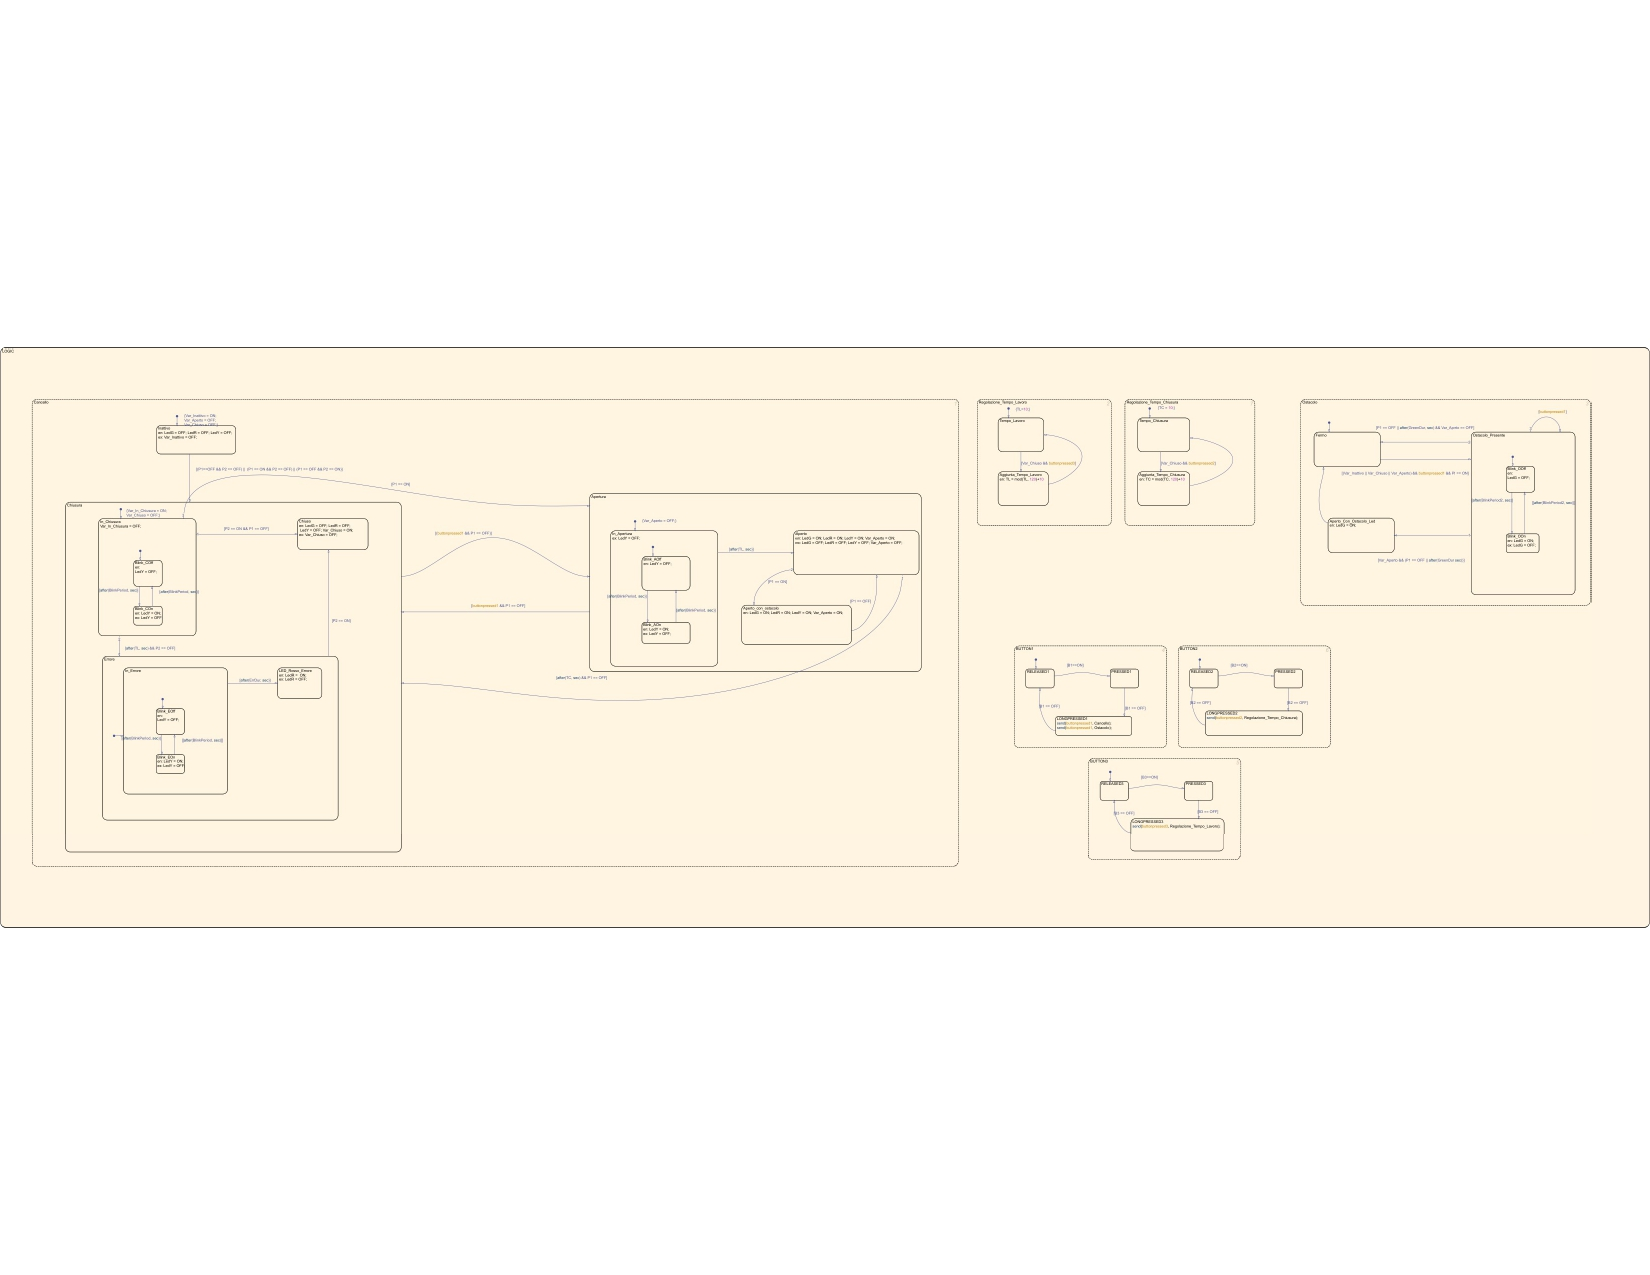
\includegraphics[width=1.5\linewidth, angle=90]{figures/final.jpg}
            \caption{Final Chart}
            \label{final}
        \end{figure}

        Il grafico finale in figura \ref{final} rappresenta il diagramma a stati nella sua interezza. Vi sono 6 macrostati che vengono eseguiti in parallelo grazie alla presenza del macrostato \textbf{LOGIC} esterno avente decomposizione \textbf{AND}.


    \section{Inputs \& Outputs}
        Il grafico in figura \ref{state1} mostra il diagramma precedente con i relativi input e output, ovvero 5 pulsanti (rispettivamente B1, B2, B3, P1, P2) e 3 LED (LedG, LedY, LedR).
        
        \noindent I pulsanti relativi ai sensori di presenza P1 e P2 sono degli switch collegati a delle costanti che vengono poste ad 1 quando il sensore si attiva e a 0 quando il sensore di disattiva.
        Anche i bottoni sono stati collegati a delle costanti ed essi sono configurati in modalità \textit{Momentary}, dunque il loro valore è normalmente 0, ma diventa 1 solo quando viene premuto.
    
        \noindent Per i LED sono stati utilizzati dei blocchi \textit{Out} collegati a blocchi \textit{Lamp} di colore verde, rosso e giallo per segnalarne la corretta accensione.
    
        \begin{figure}[H]
            \centering
            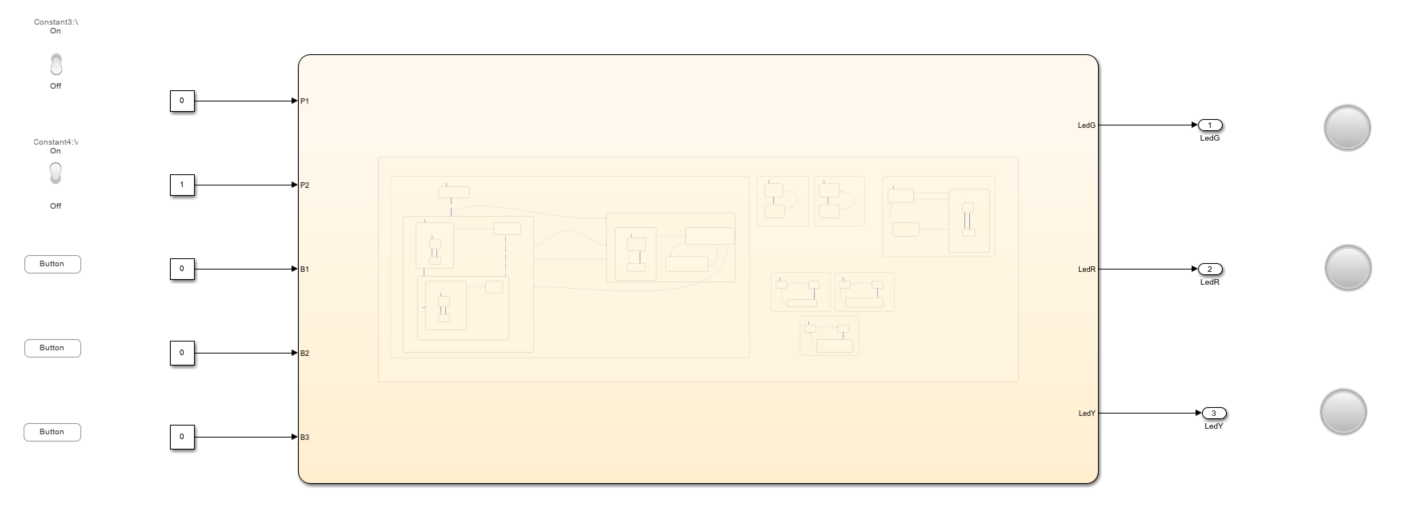
\includegraphics[width=0.9\textwidth]{figures/state.png}
            \caption{Input e Output}
            \label{state1}
        \end{figure}
    \chapter{Test Simulink}
    In questo capitolo ci concentreremo su verifica e validazione del diagramma a stati attraverso l'utilizzo di Simulink Test in Simulink. Essi permettono di isolare e testare singoli componenti del modello, garantendo che ogni parte del sistema funzioni correttamente. Esploreremo le tecniche per creare, configurare ed eseguire test dettagliati e analizzare i risultati per identificare e correggere eventuali errori. Questo processo è fondamentale per assicurare l'affidabilità e l'accuratezza del modello complessivo, consentendo di simulare scenari diversi e verificare il comportamento del sistema in condizioni variabili.

    \begin{figure}[H]
        \centering
        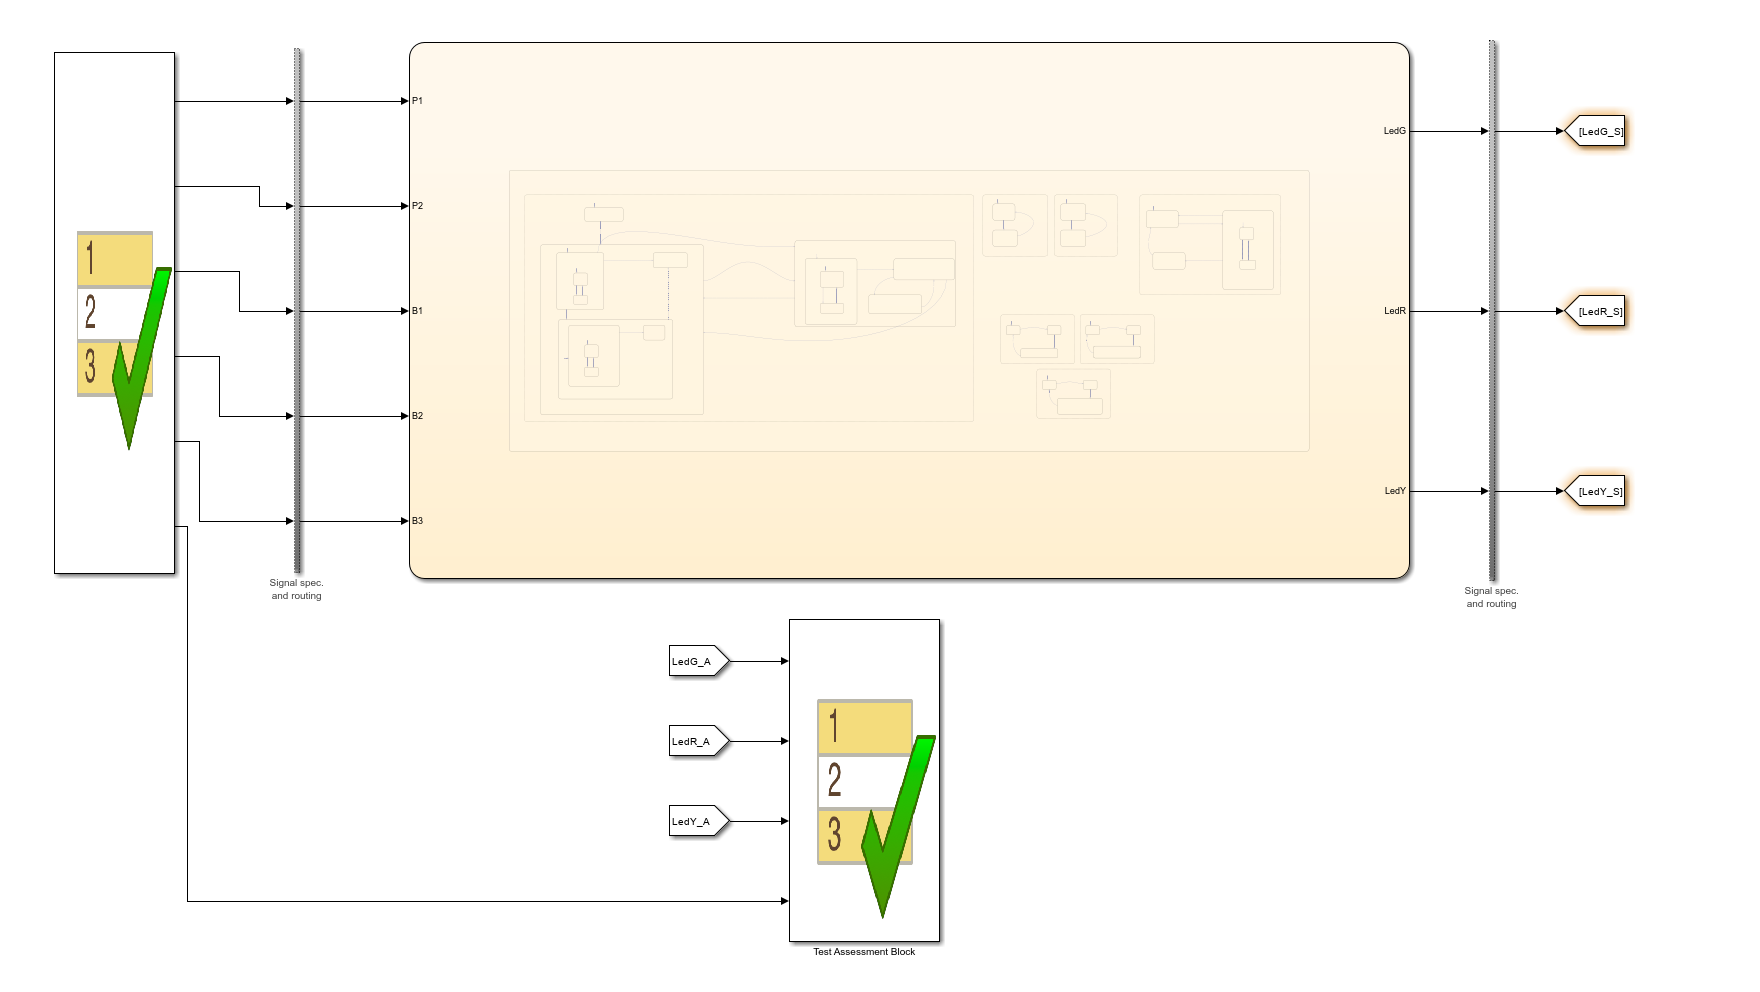
\includegraphics[width=0.6\textwidth]{figures/testharness.png}
        \caption{Esempio Test Harness}
        \label{harness}
    \end{figure}


    \section{Test Apertura e Chiusura Cancello}
        Di seguito è riportato il test relativo alla verifica della corretta apertura e chiusura del cancello quando l'utente preme il pulsante B1. In particolare, si effettua la verifica del corretto lampeggio del LED giallo in fase di verifica, della totale accensione di tutti i LED in fase di apertura e del totale spegnimento di questi ultimi in fase di chiusura.

        \begin{figure}[H]
            \centering
            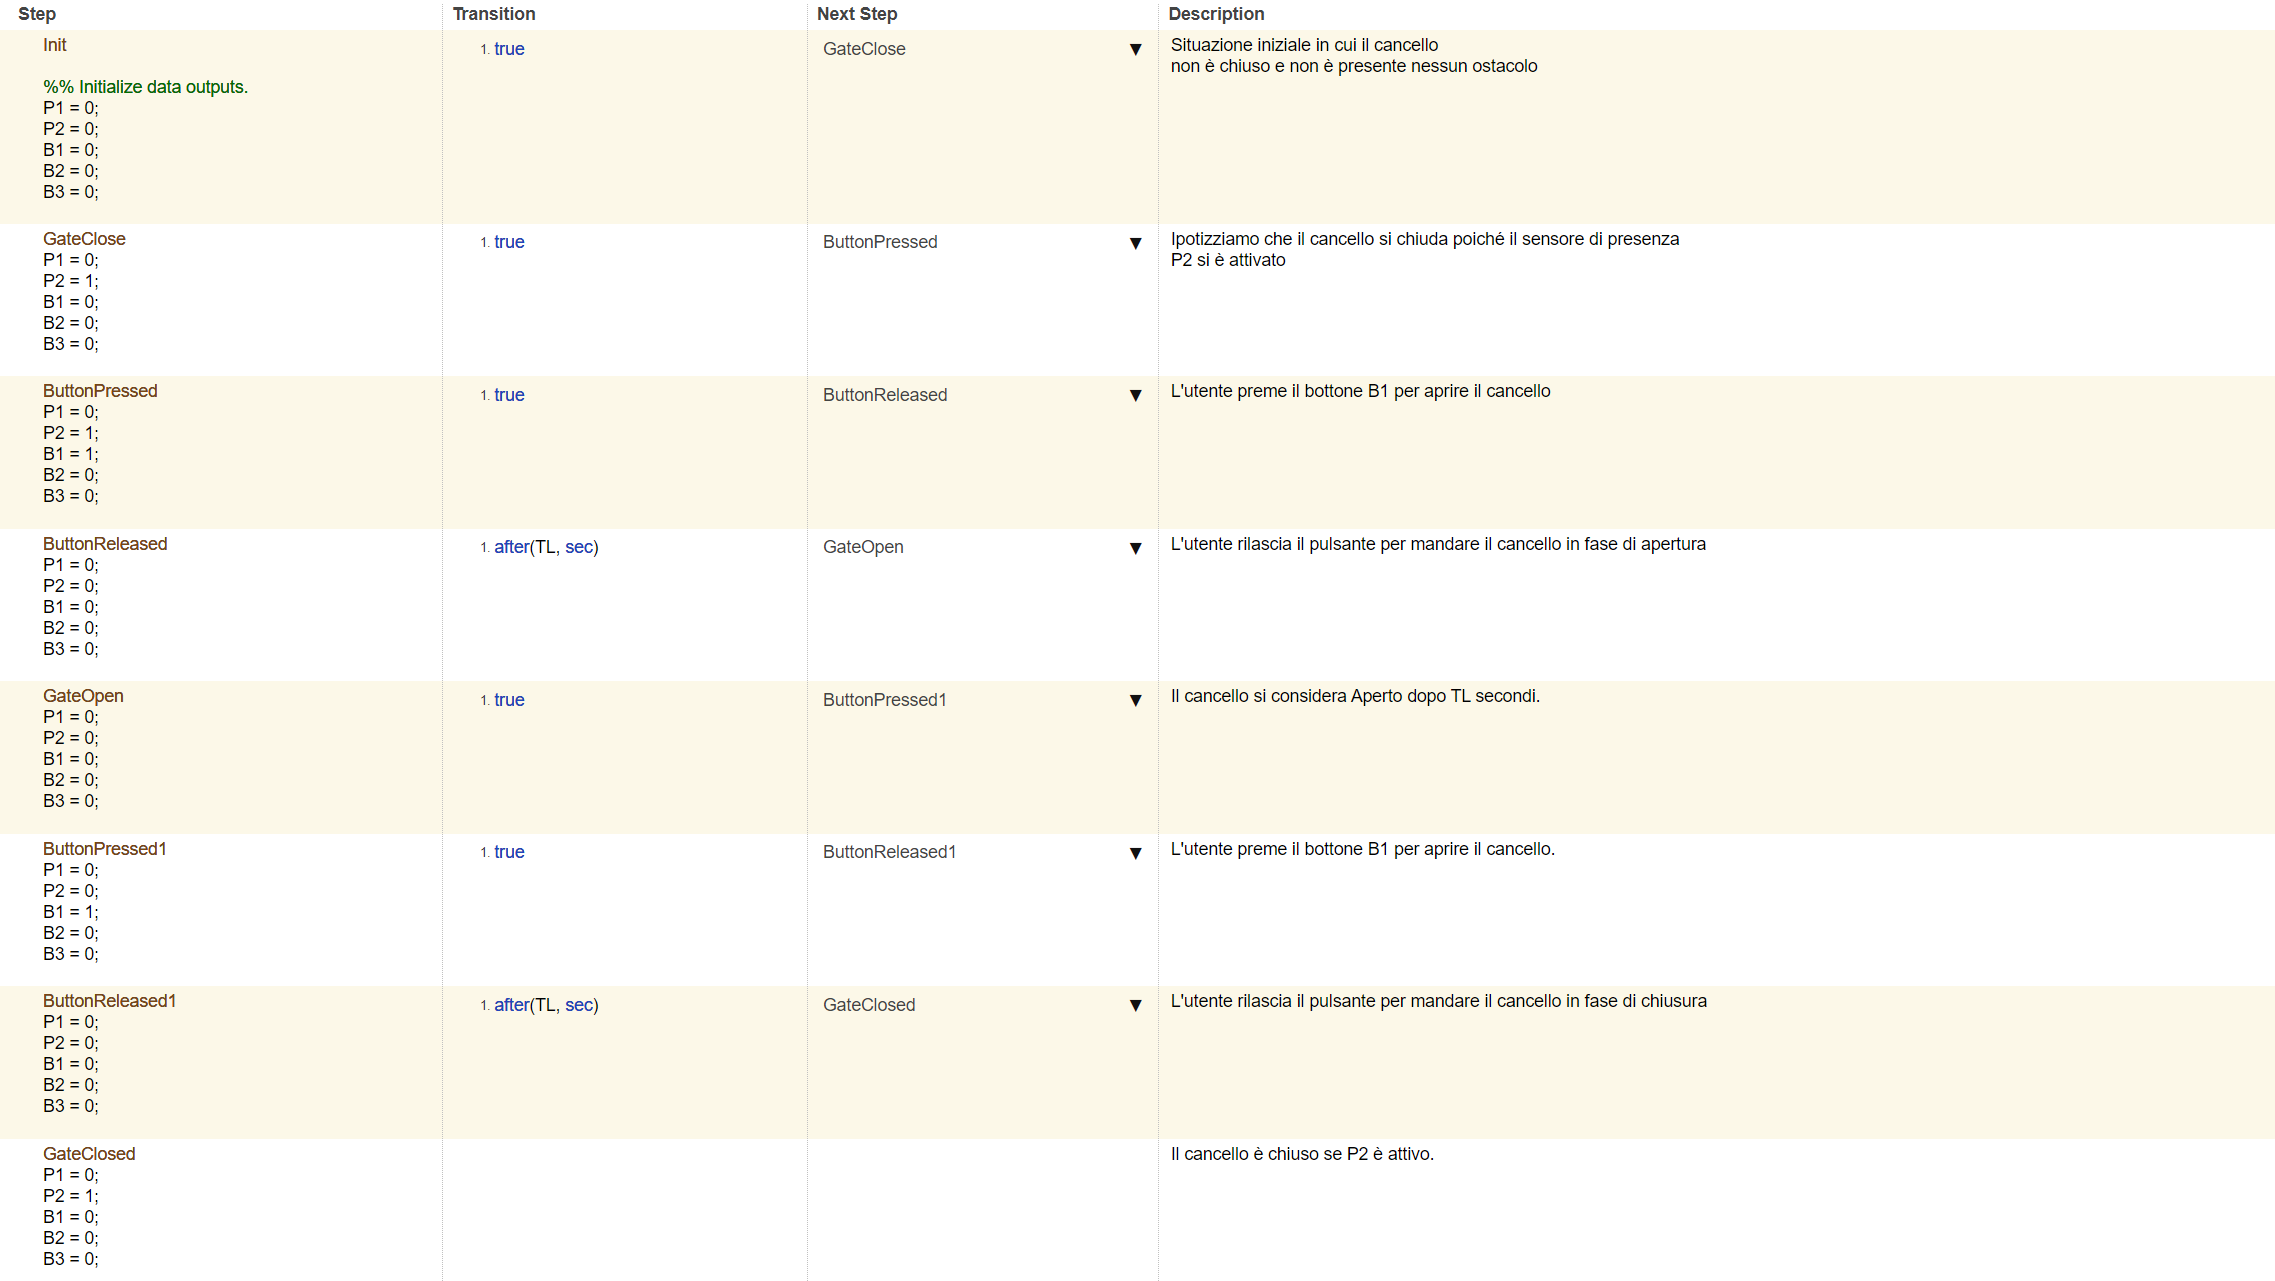
\includegraphics[width=0.9\textwidth]{figures/open_close.png}
            \caption{Test Sequence}
            \label{openclose}
        \end{figure}
    
        \begin{figure}[H]
            \centering
            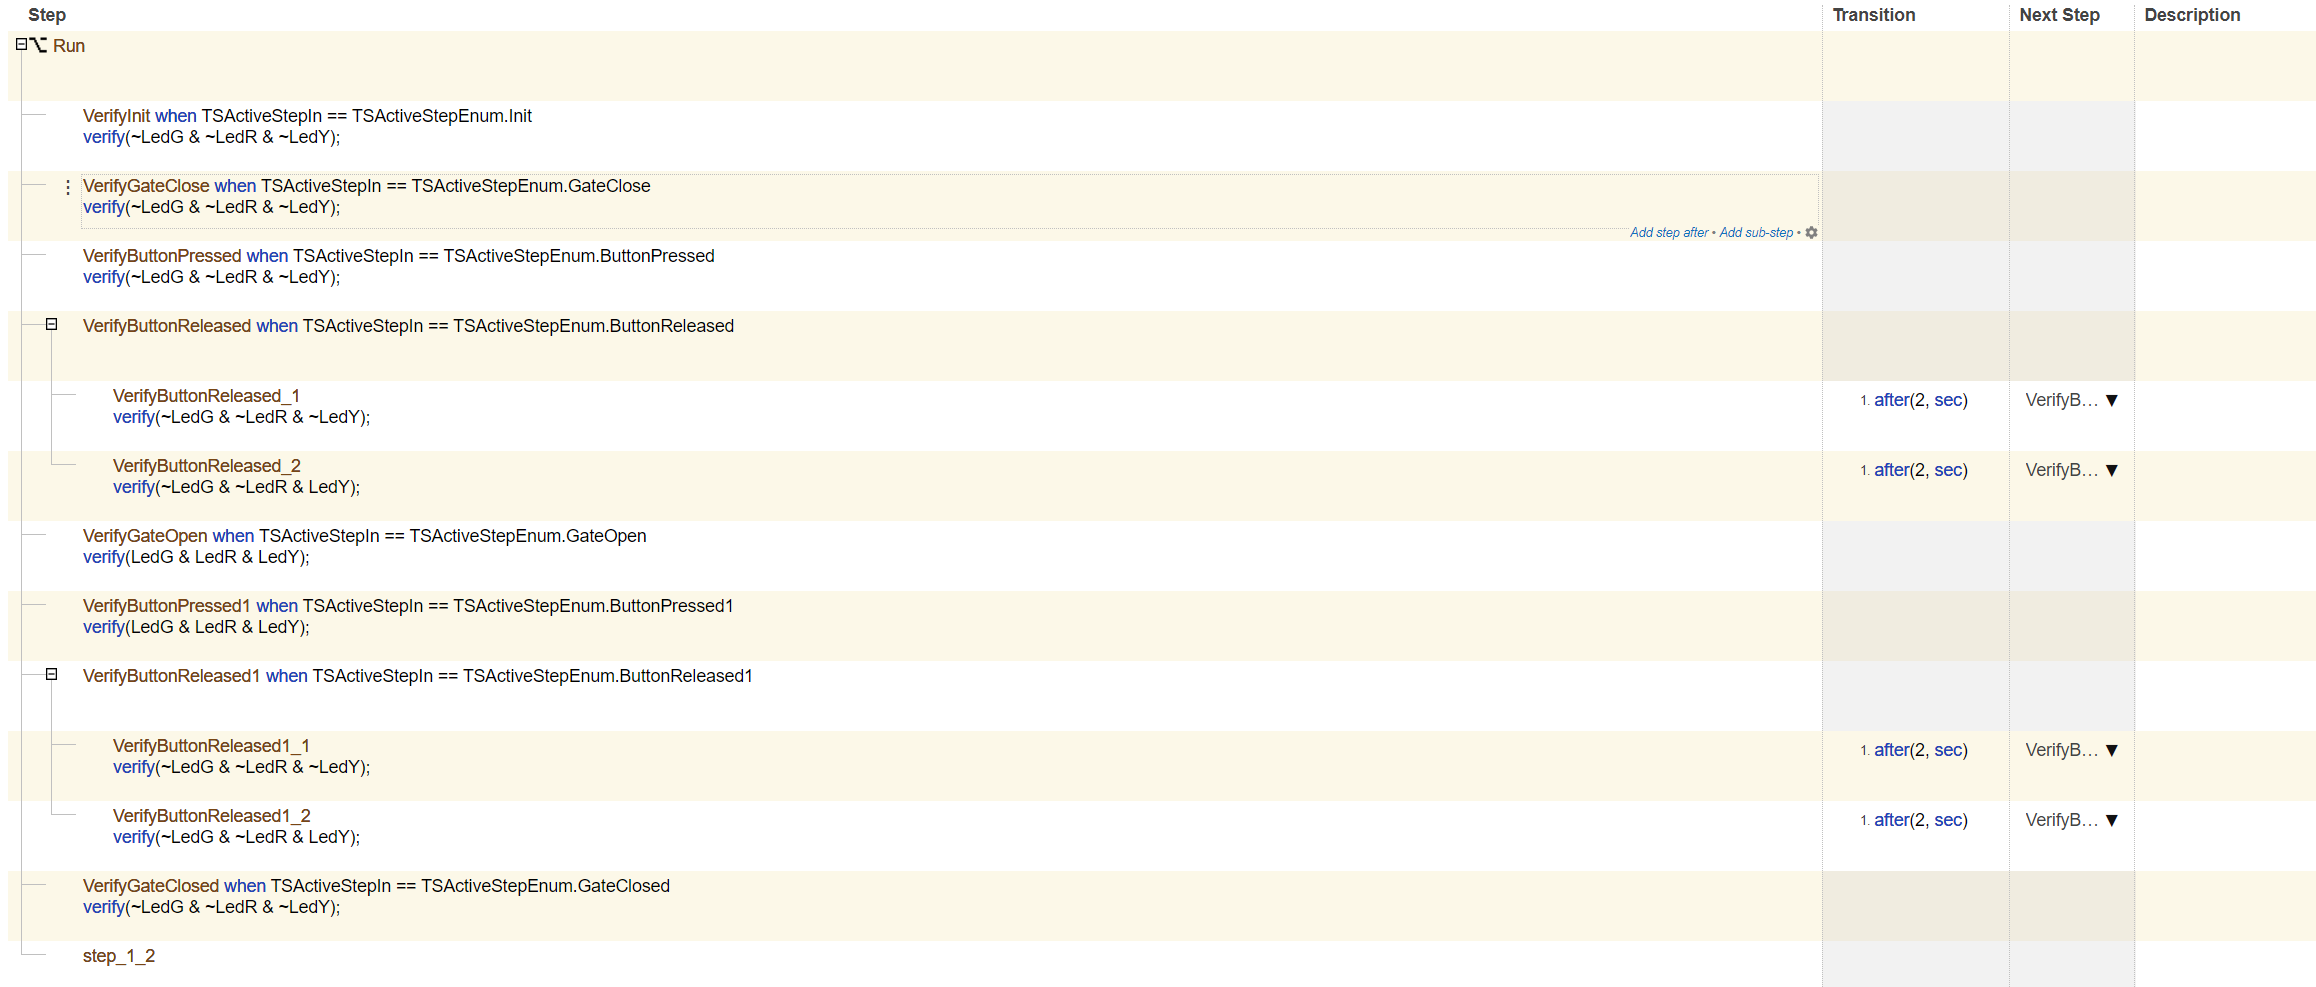
\includegraphics[width=0.9\textwidth]{figures/open_close2.png}
            \caption{Test Assessment}
            \label{openclose2}
        \end{figure}


    \section{Test Errore Cancello}
        Si riporta il test relativo alla verifica dello stato di errore del cancello qualora il sensore di presenza P2 non si attivi dopo $T_L$ secondi durante la fase di chiusura.
        Si ricorda che, dopo aver atteso tale tempo, il dispositivo attende ulteriori 10 secondi prima di accendere il LED rosso e segnalare la definitiva permanenza nello stato di errore.

        \begin{figure}[H]
            \centering
            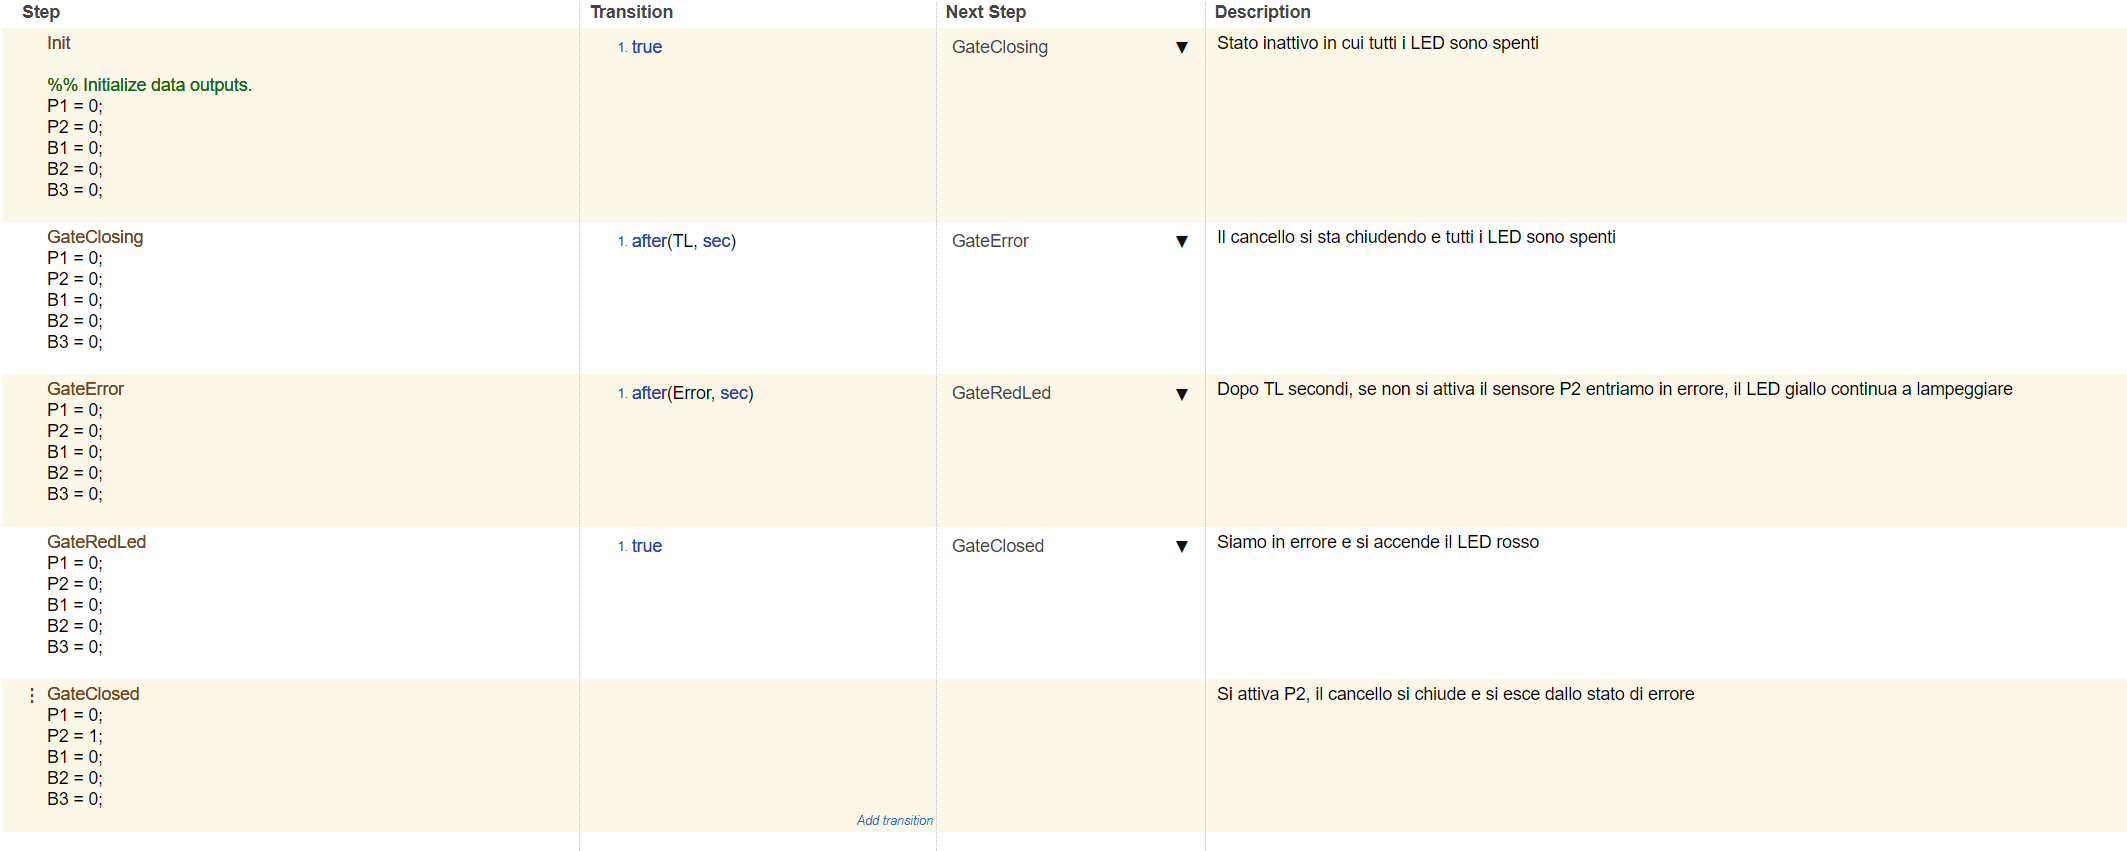
\includegraphics[width=0.9\textwidth]{figures/error.png}
            \caption{Test Sequence}
            \label{error}
        \end{figure}
    
        \begin{figure}[H]
            \centering
            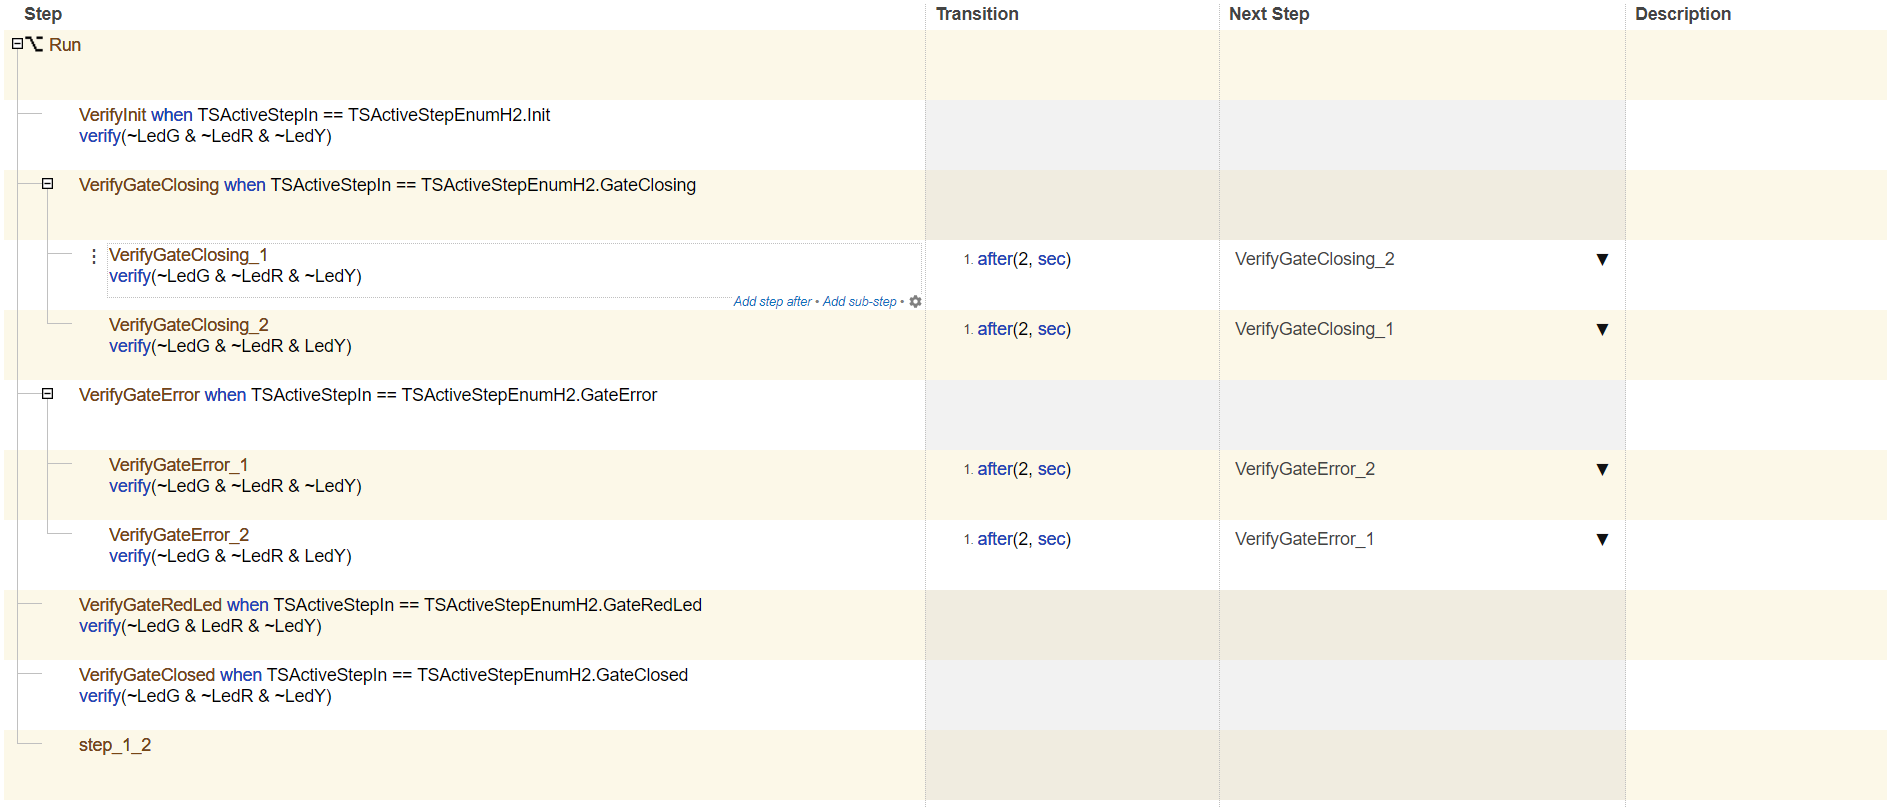
\includegraphics[width=0.9\textwidth]{figures/error2.png}
            \caption{Test Assessment}
            \label{error2}
        \end{figure}


    \section{Test Rilevazione Ostacolo se Aperto}
        Si riporta il test relativo alla rilevazione di un ostacolo quando il cancello si trova nello stato \textbf{Aperto}. Si ricorda che in caso di rilevazione positiva, mentre il cancello si sposta nello stato \textbf{Aperto con Ostacolo}, il macrostato \textbf{Ostacolo} permette il lampeggio del LED verde per un periodo di 30 secondi se l'utente tenta di chiudere il cancello con il sensore P1 attivo. 

        \begin{figure}[H]
            \centering
            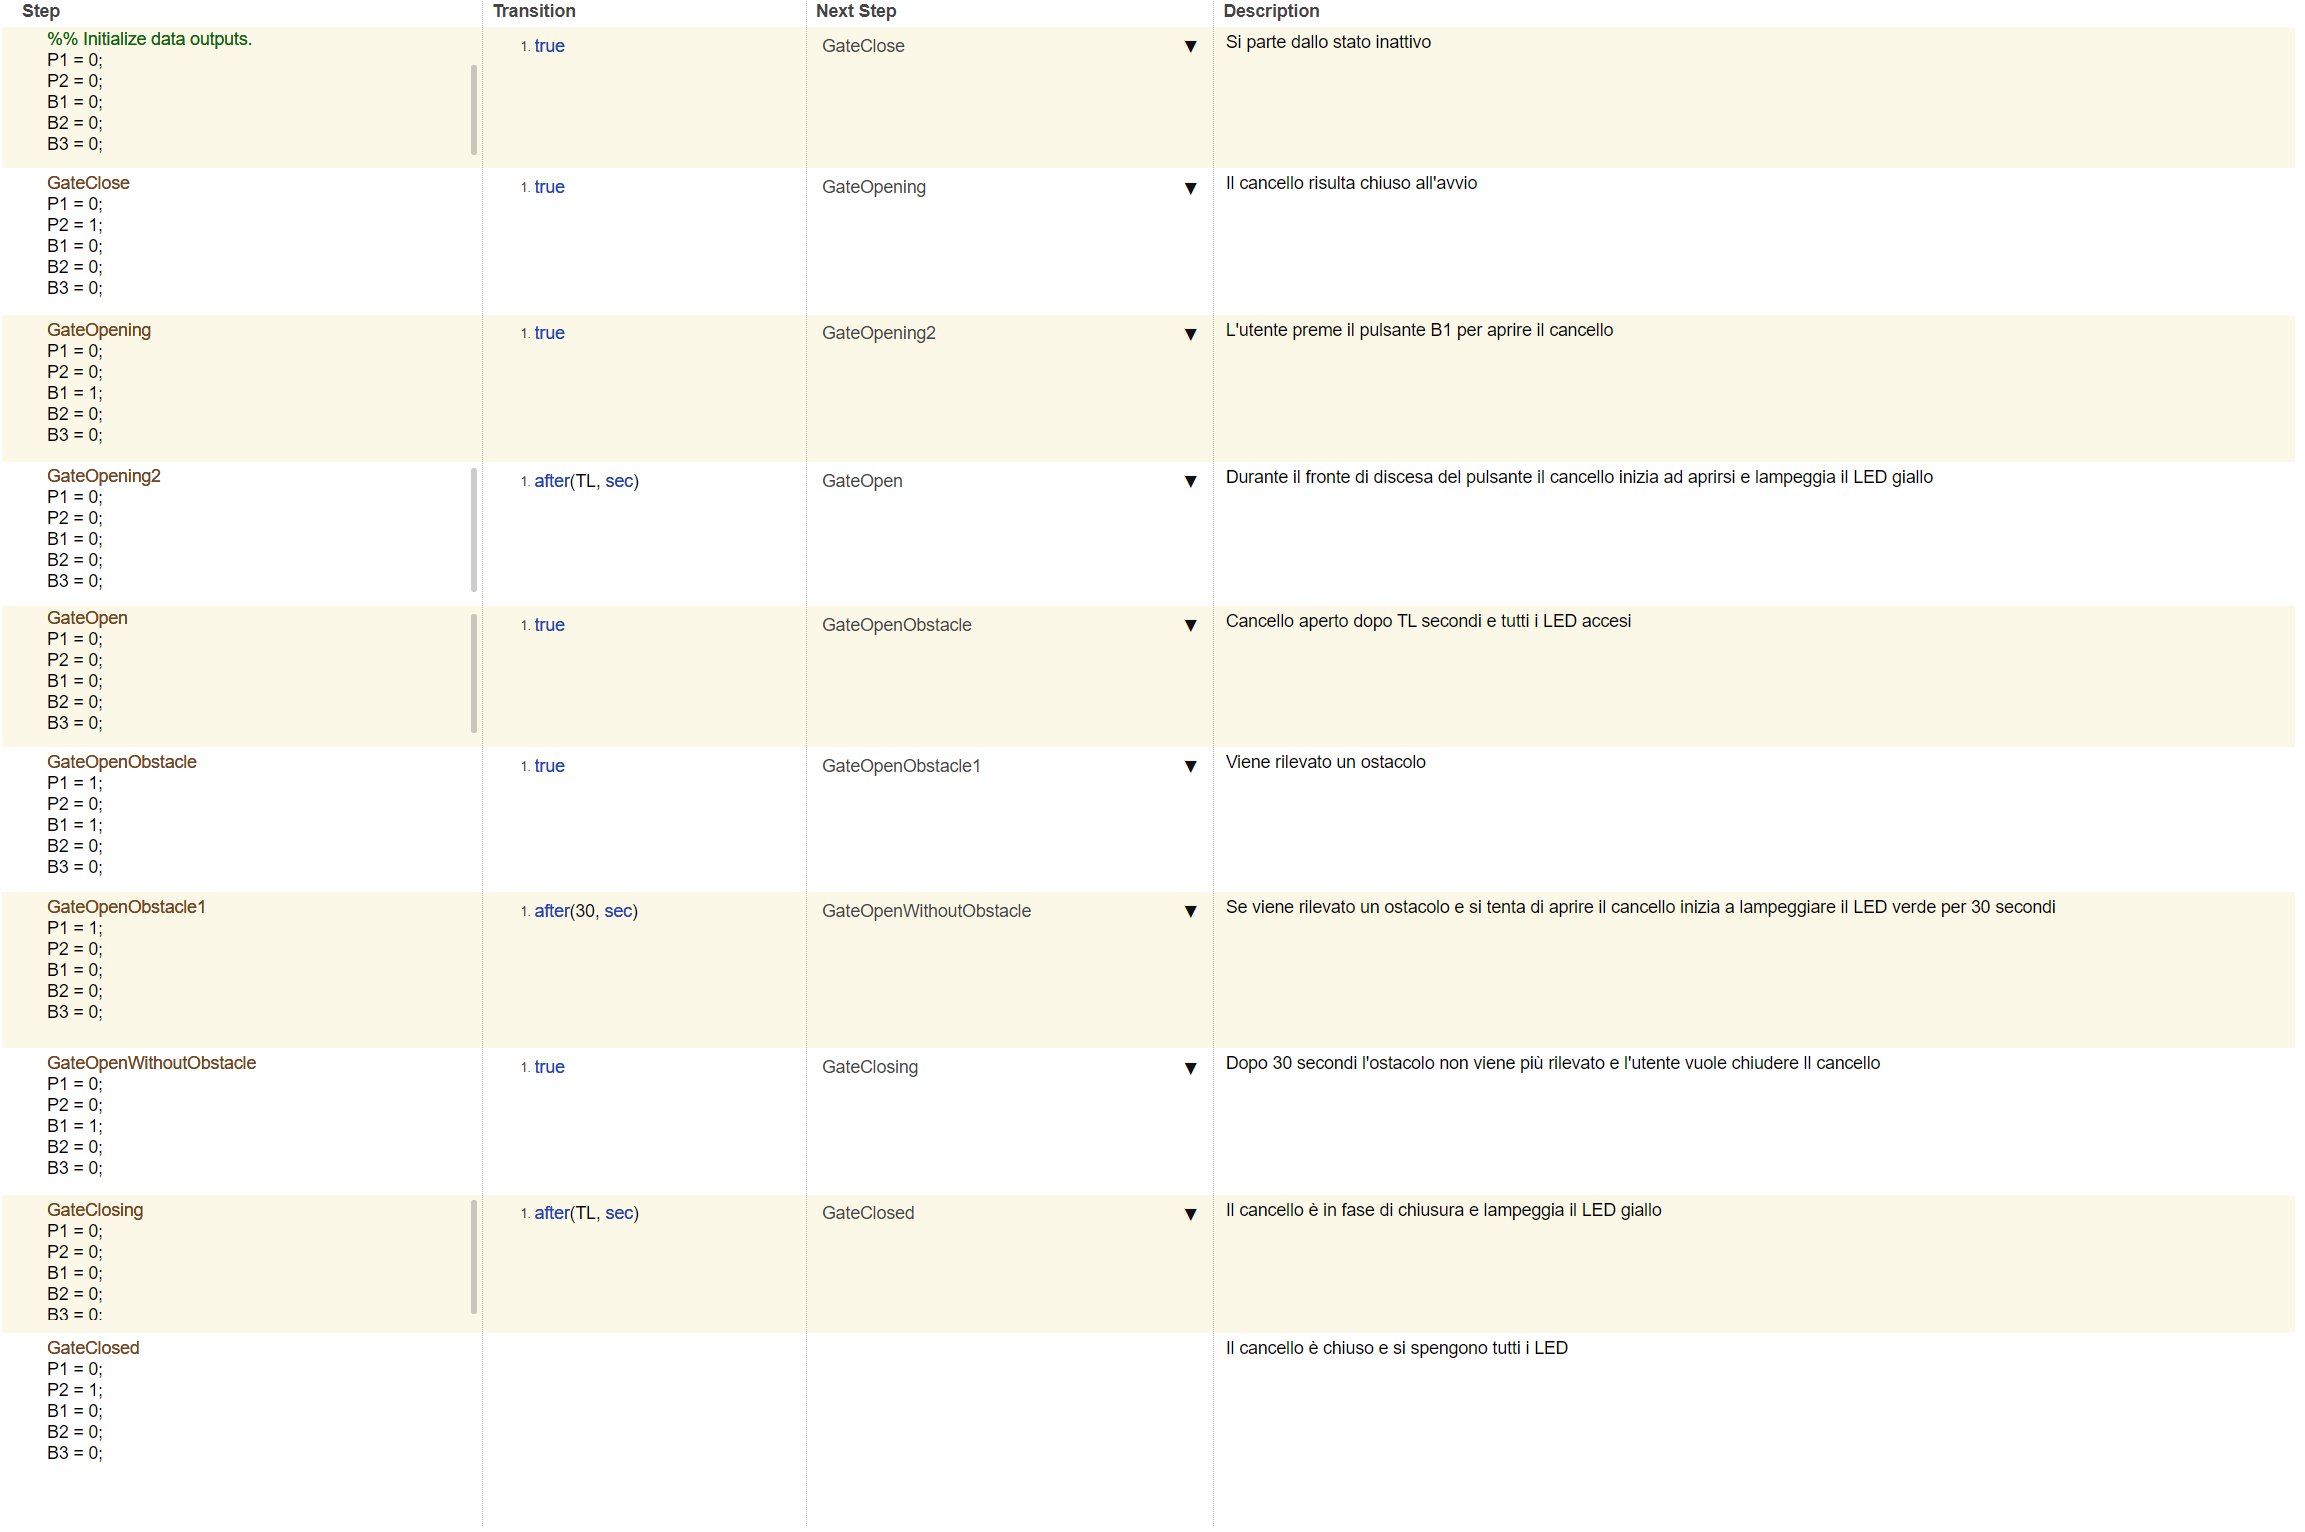
\includegraphics[width=0.9\textwidth]{figures/obstacletest.png}
            \caption{Test Sequence}
            \label{obtest}
        \end{figure}
    
        \begin{figure}[H]
            \centering
            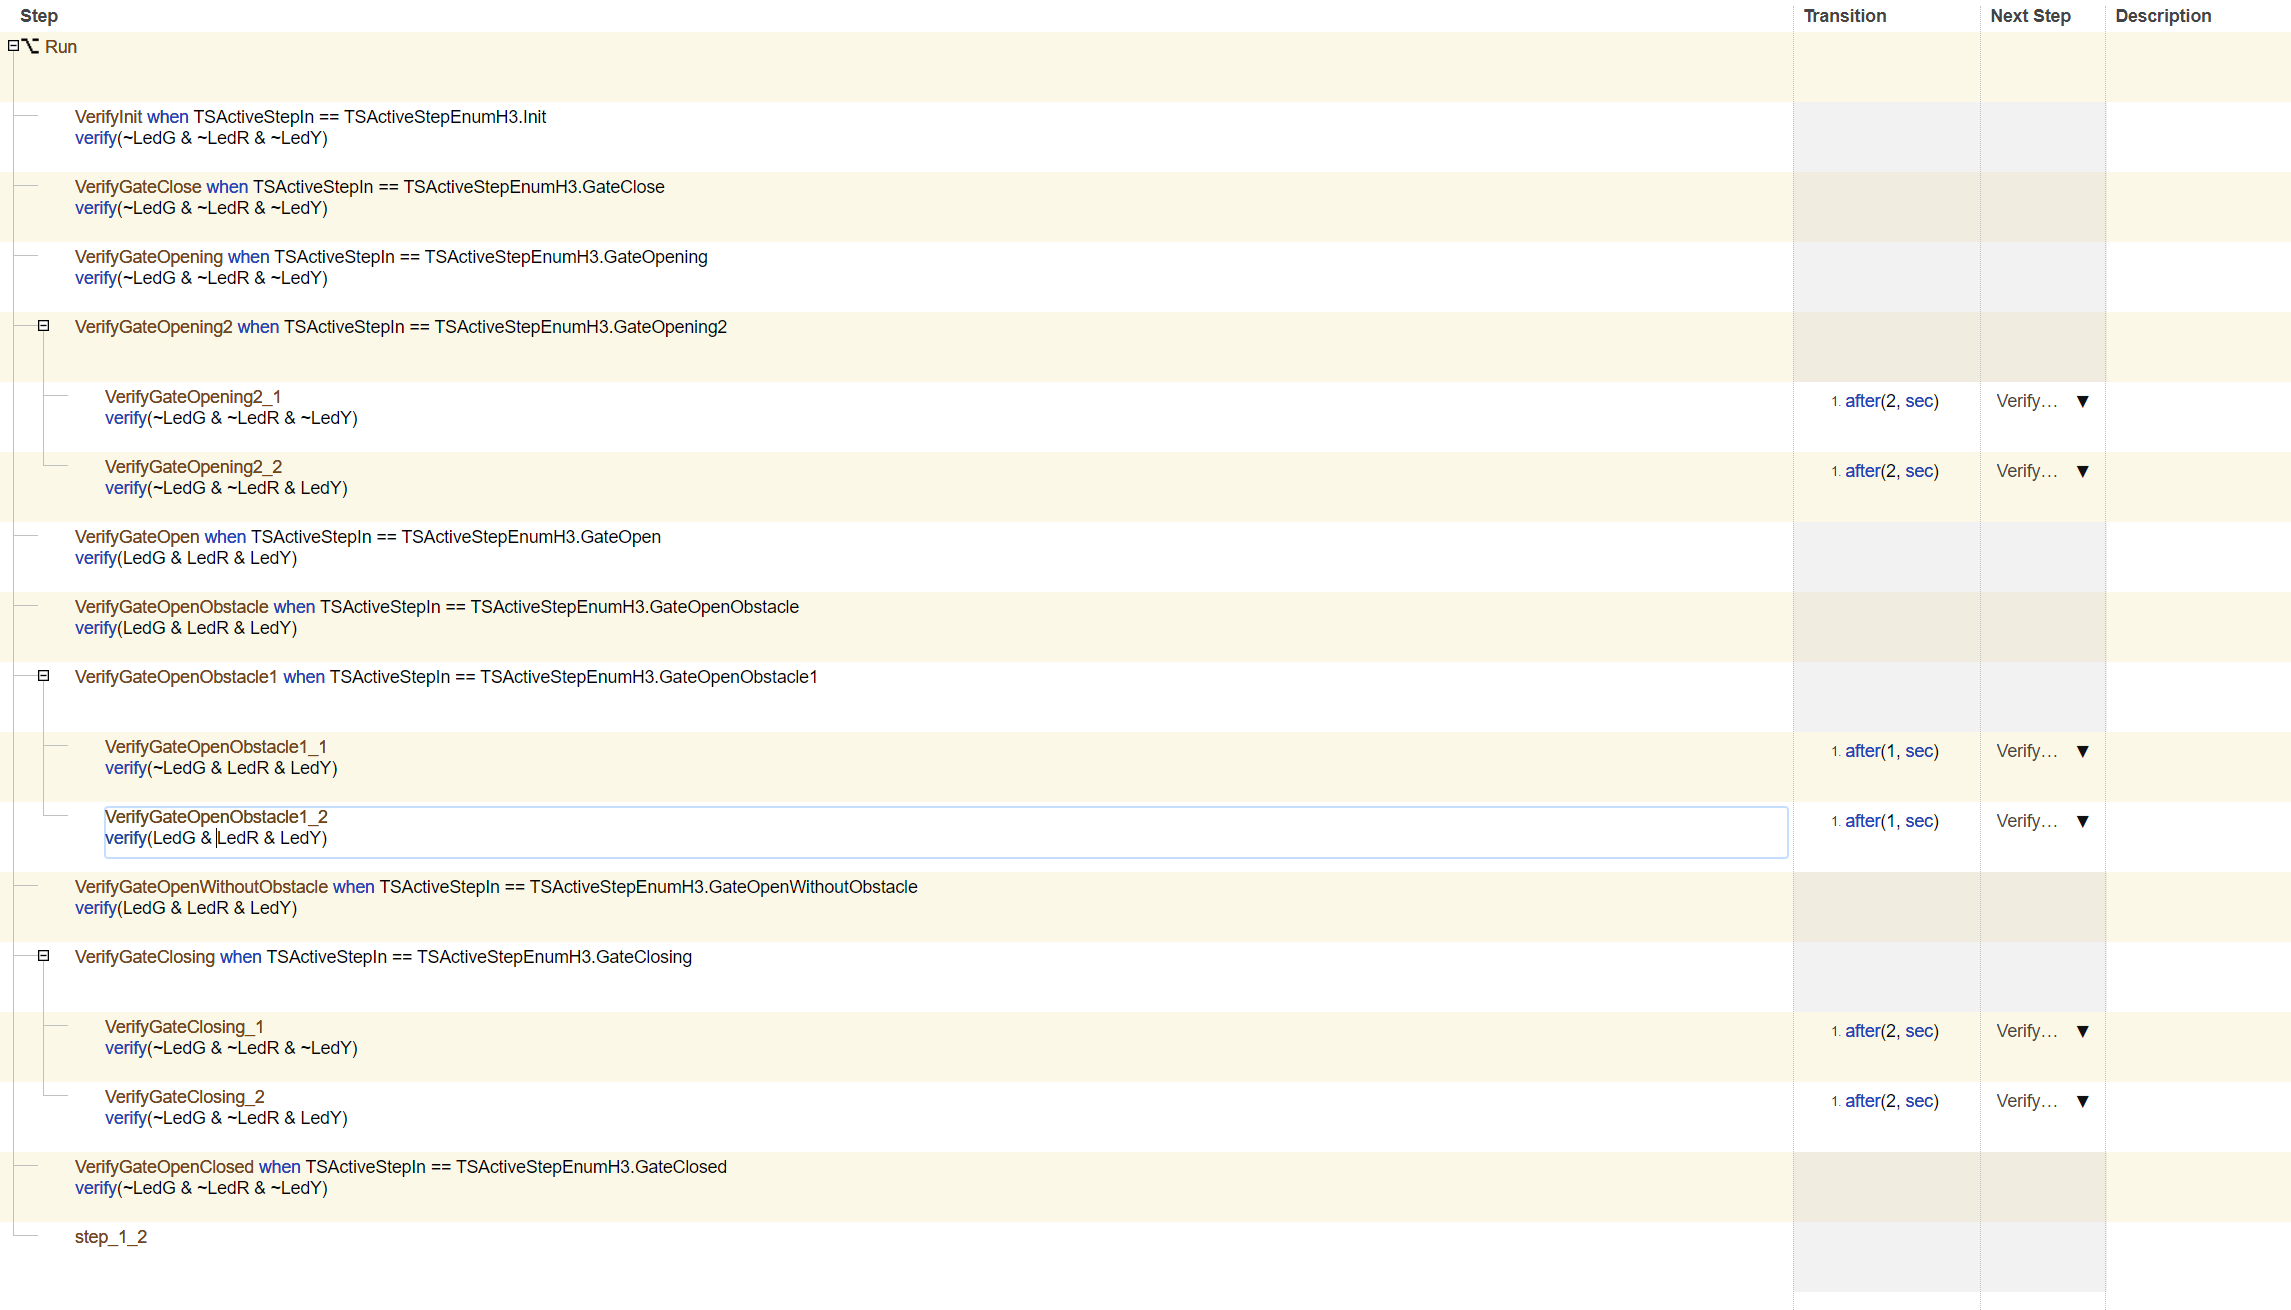
\includegraphics[width=0.9\textwidth]{figures/obstacletest1.png}
            \caption{Test Assessment}
            \label{obstest1}
        \end{figure}


    \section{Test Rilevazione Ostacolo se In Chiusura}
        Si riporta il test relativo alla rilevazione di un ostacolo quando il cancello è in fase di chiusura.
        In particolare, il cancello si sposta in fase di apertura continuando il lampeggio del LED giallo per poi aprirsi completamente.
        In seguito, il test prevede l'attesa del tempo di chiusura automatica $T_C$ per poi chiudersi definitivamente.

        \begin{figure}[H]
            \centering
            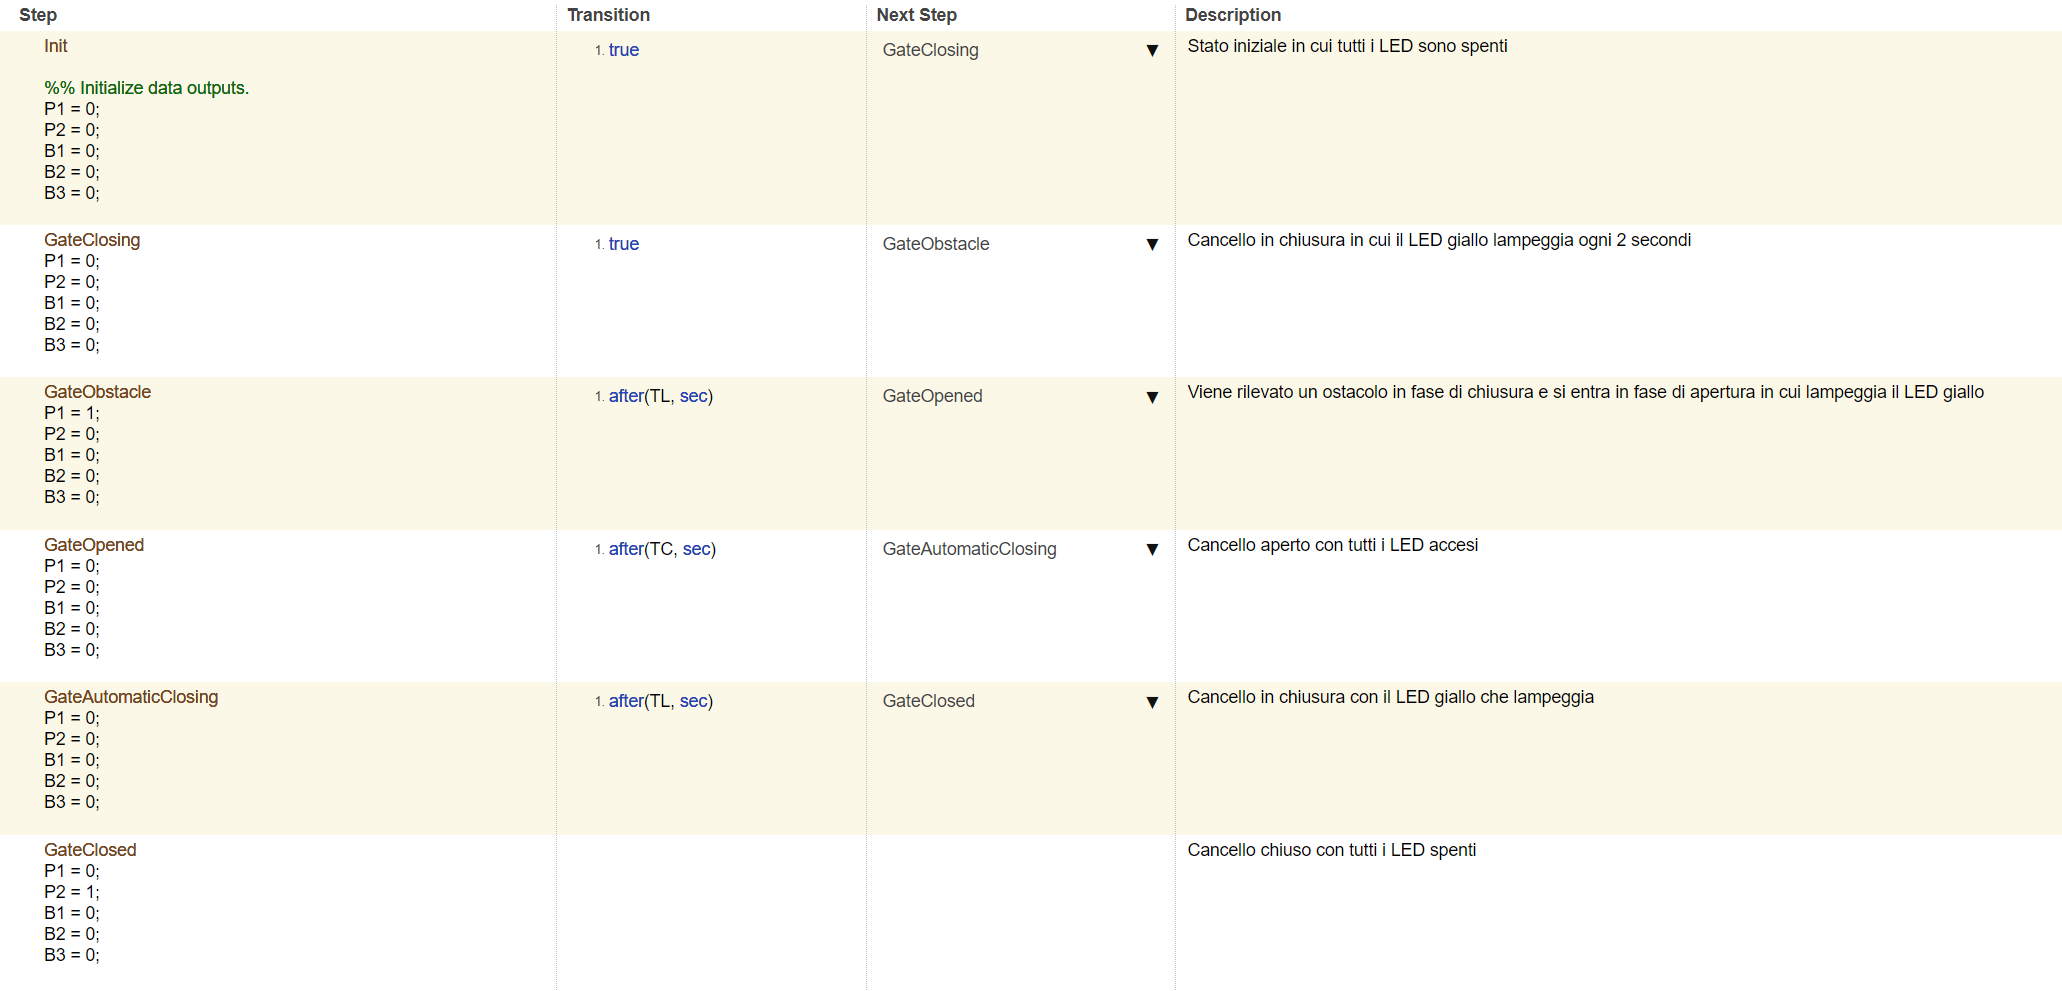
\includegraphics[width=0.9\textwidth]{figures/automaticclosing.png}
            \caption{Test Sequence}
            \label{autom}
        \end{figure}
        
        \begin{figure}[H]
            \centering
            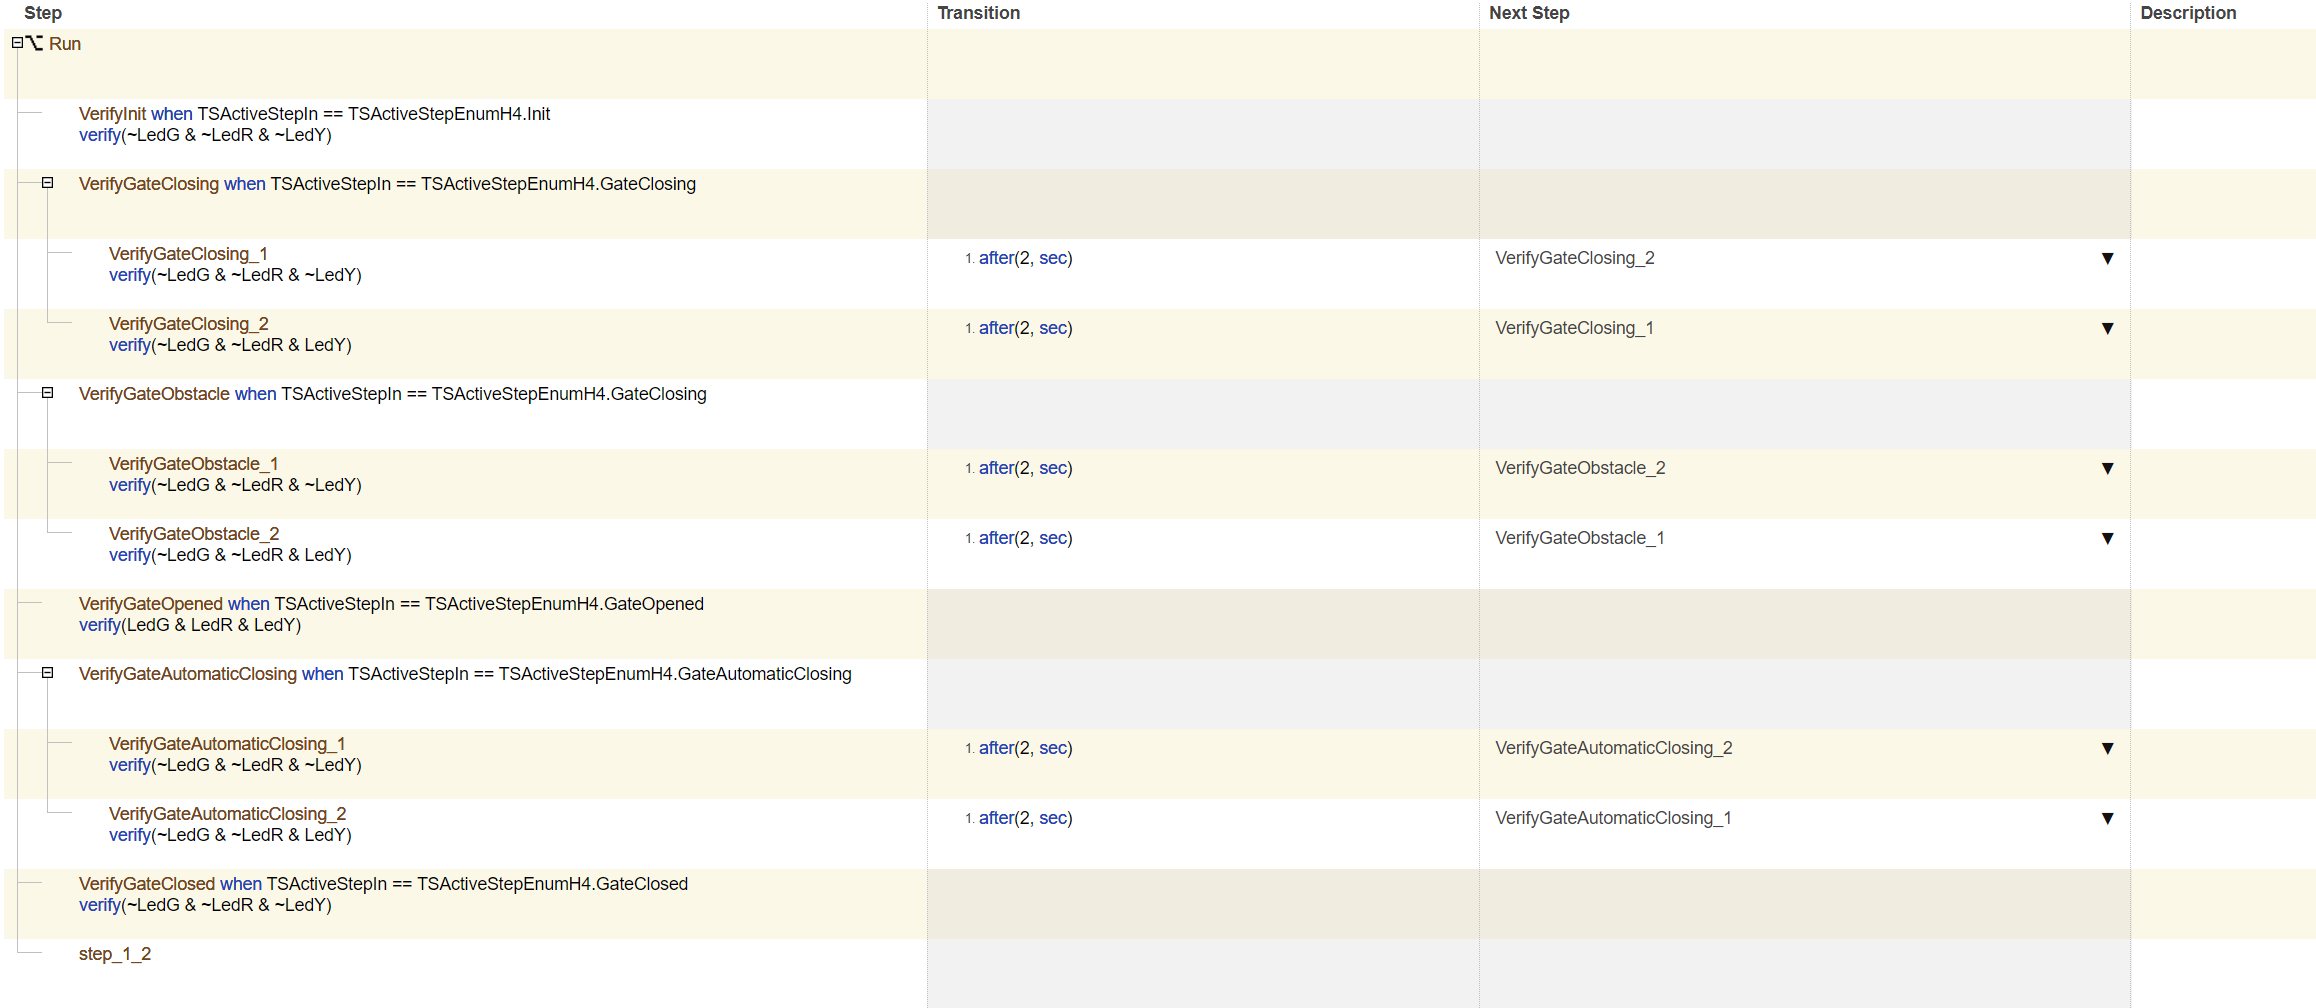
\includegraphics[width=0.9\textwidth]{figures/automaticclosing1.png}
            \caption{Test Assessment}
            \label{autom1}
        \end{figure}

    
    \section{Test Rilevazione Ostacolo se Chiuso}
        Si riporta il test relativo alla rilevazione di un ostacolo quando il cancello è chiuso. In particolare, il cancello non si apre se l'utente preme il pulsante B1, ma inizia il lampeggio del LED verde per 30 secondi, per poi spegnersi insieme agli altri due LED.

        \begin{figure}[H]
            \centering
            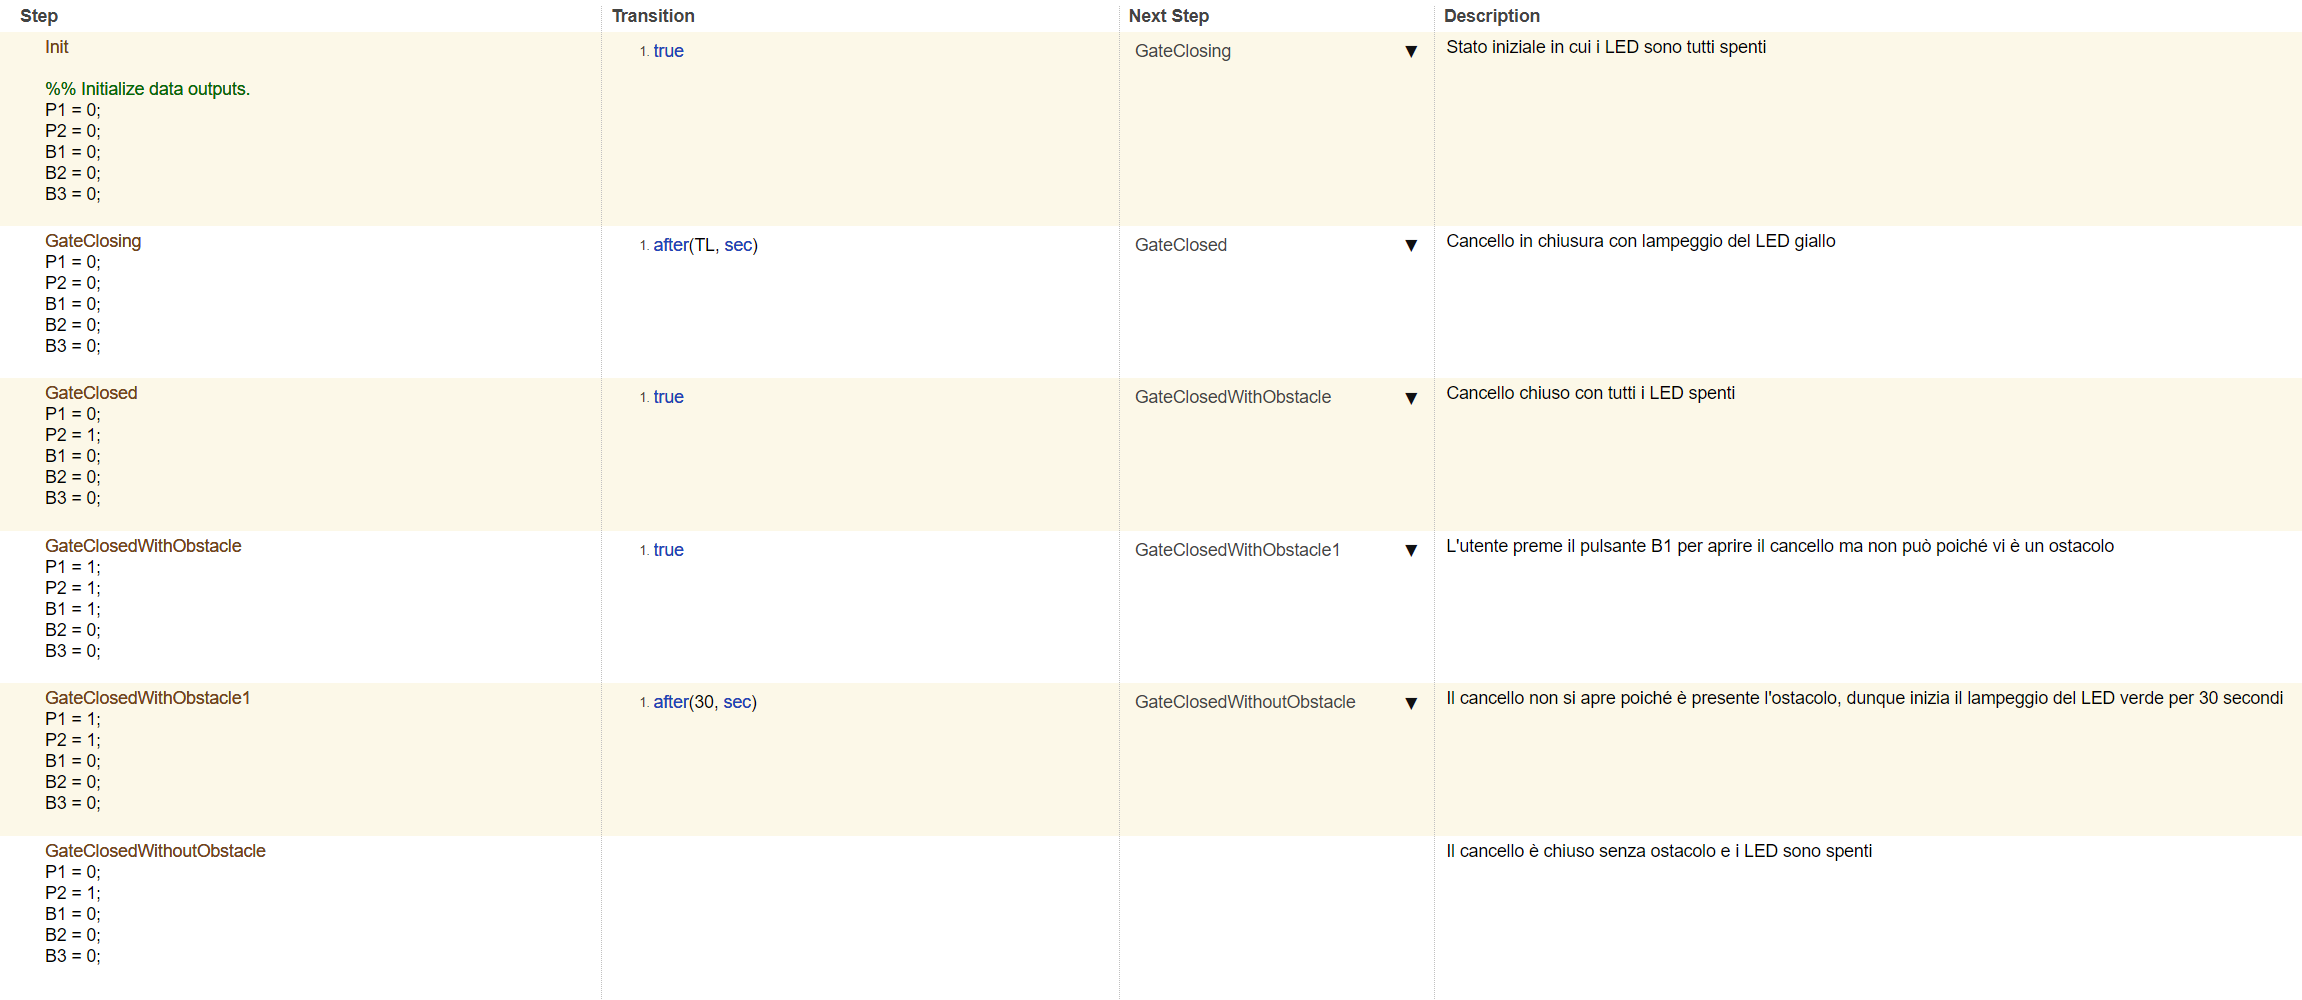
\includegraphics[width=0.9\textwidth]{figures/closedobs.png}
            \caption{Test Sequence}
            \label{closeobs}
        \end{figure}
        
        \begin{figure}[H]
            \centering
            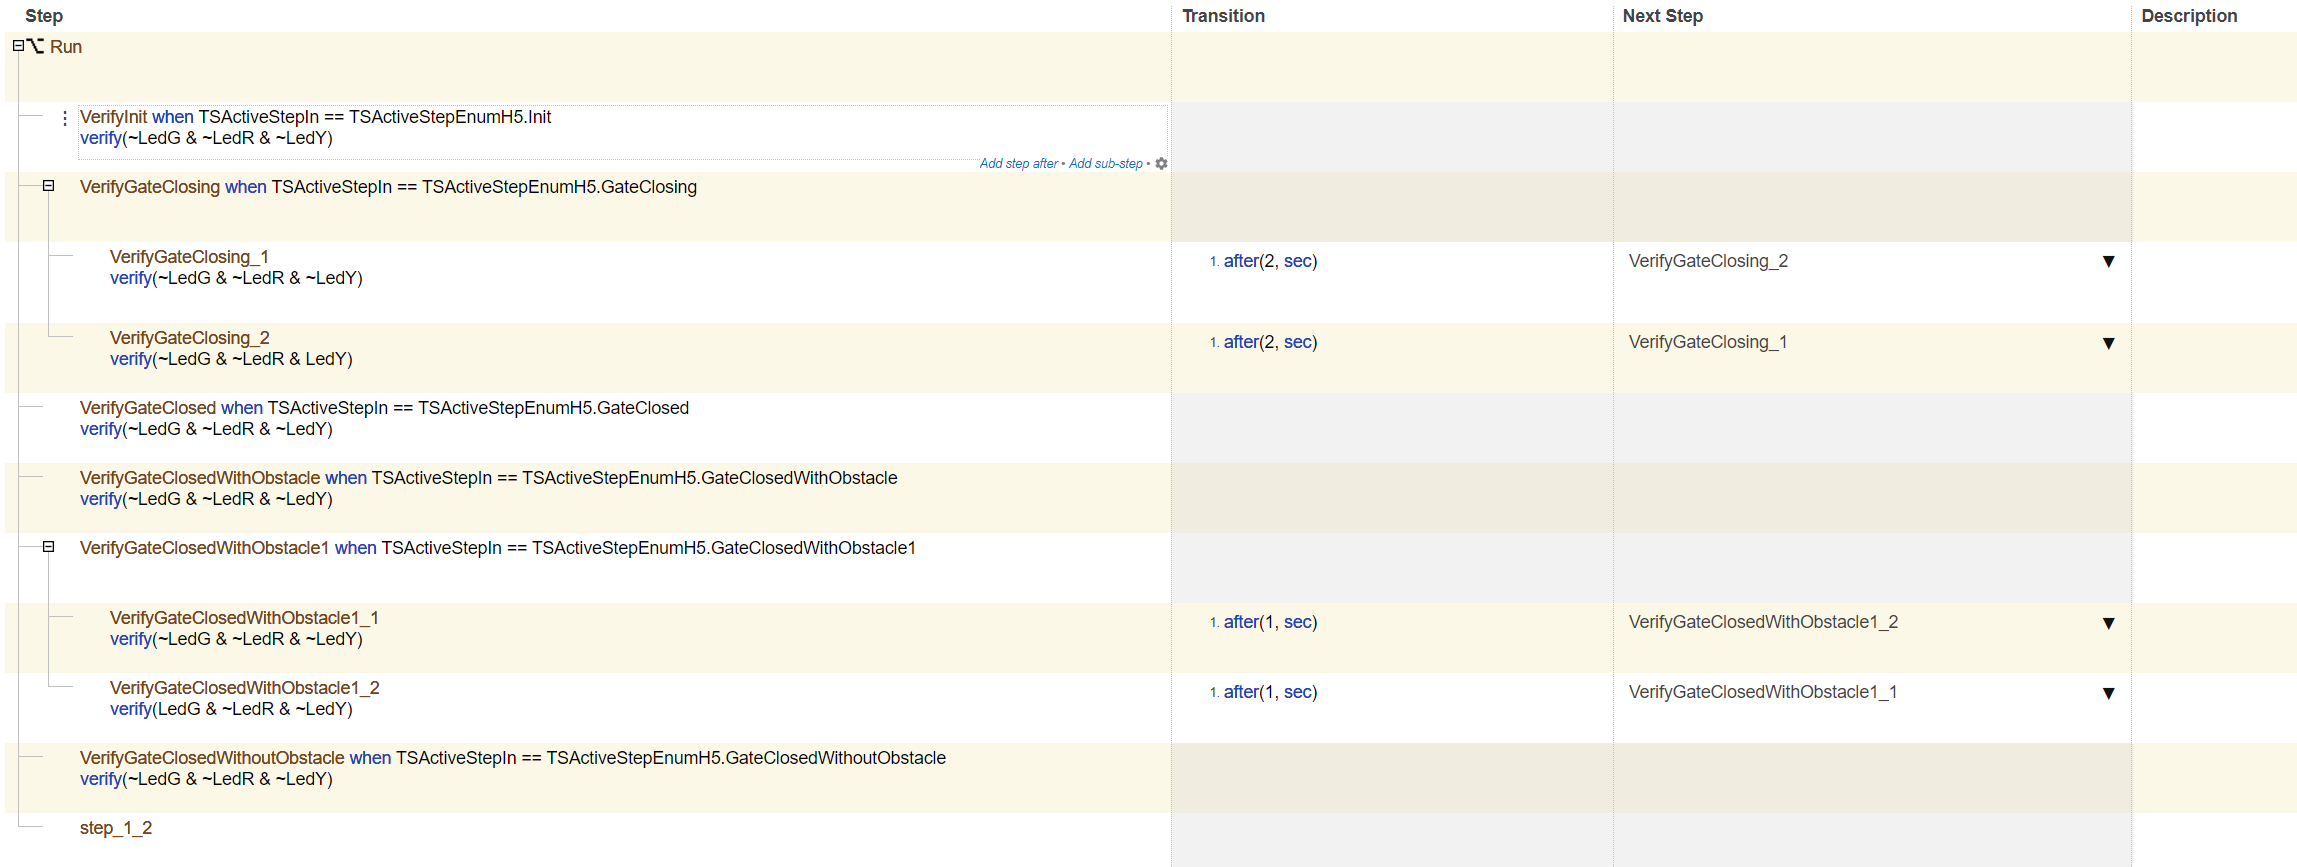
\includegraphics[width=0.9\textwidth]{figures/closedobs1.png}
            \caption{Test Assessment}
            \label{closeobs1}
        \end{figure}

    
    \section{Regolazione $T_C$ e $T_L$}
        Si riporta il test relativo alla regolazione del tempo di lavoro e del tempo di chiusura.
        In particolare, il cancello si chiude inizialmente con $T_L$ pari a 10 secondi.
        In seguito, l'utente preme il pulsante B2 e B3 per aumentare sia $T_L$ che $T_C$ di 10 secondi.
        Dopodiché, il cancello viene portato in fase di apertura (e successivamente chiusura) con il nuovo tempo di lavoro.

        \begin{figure}[H]
            \centering
            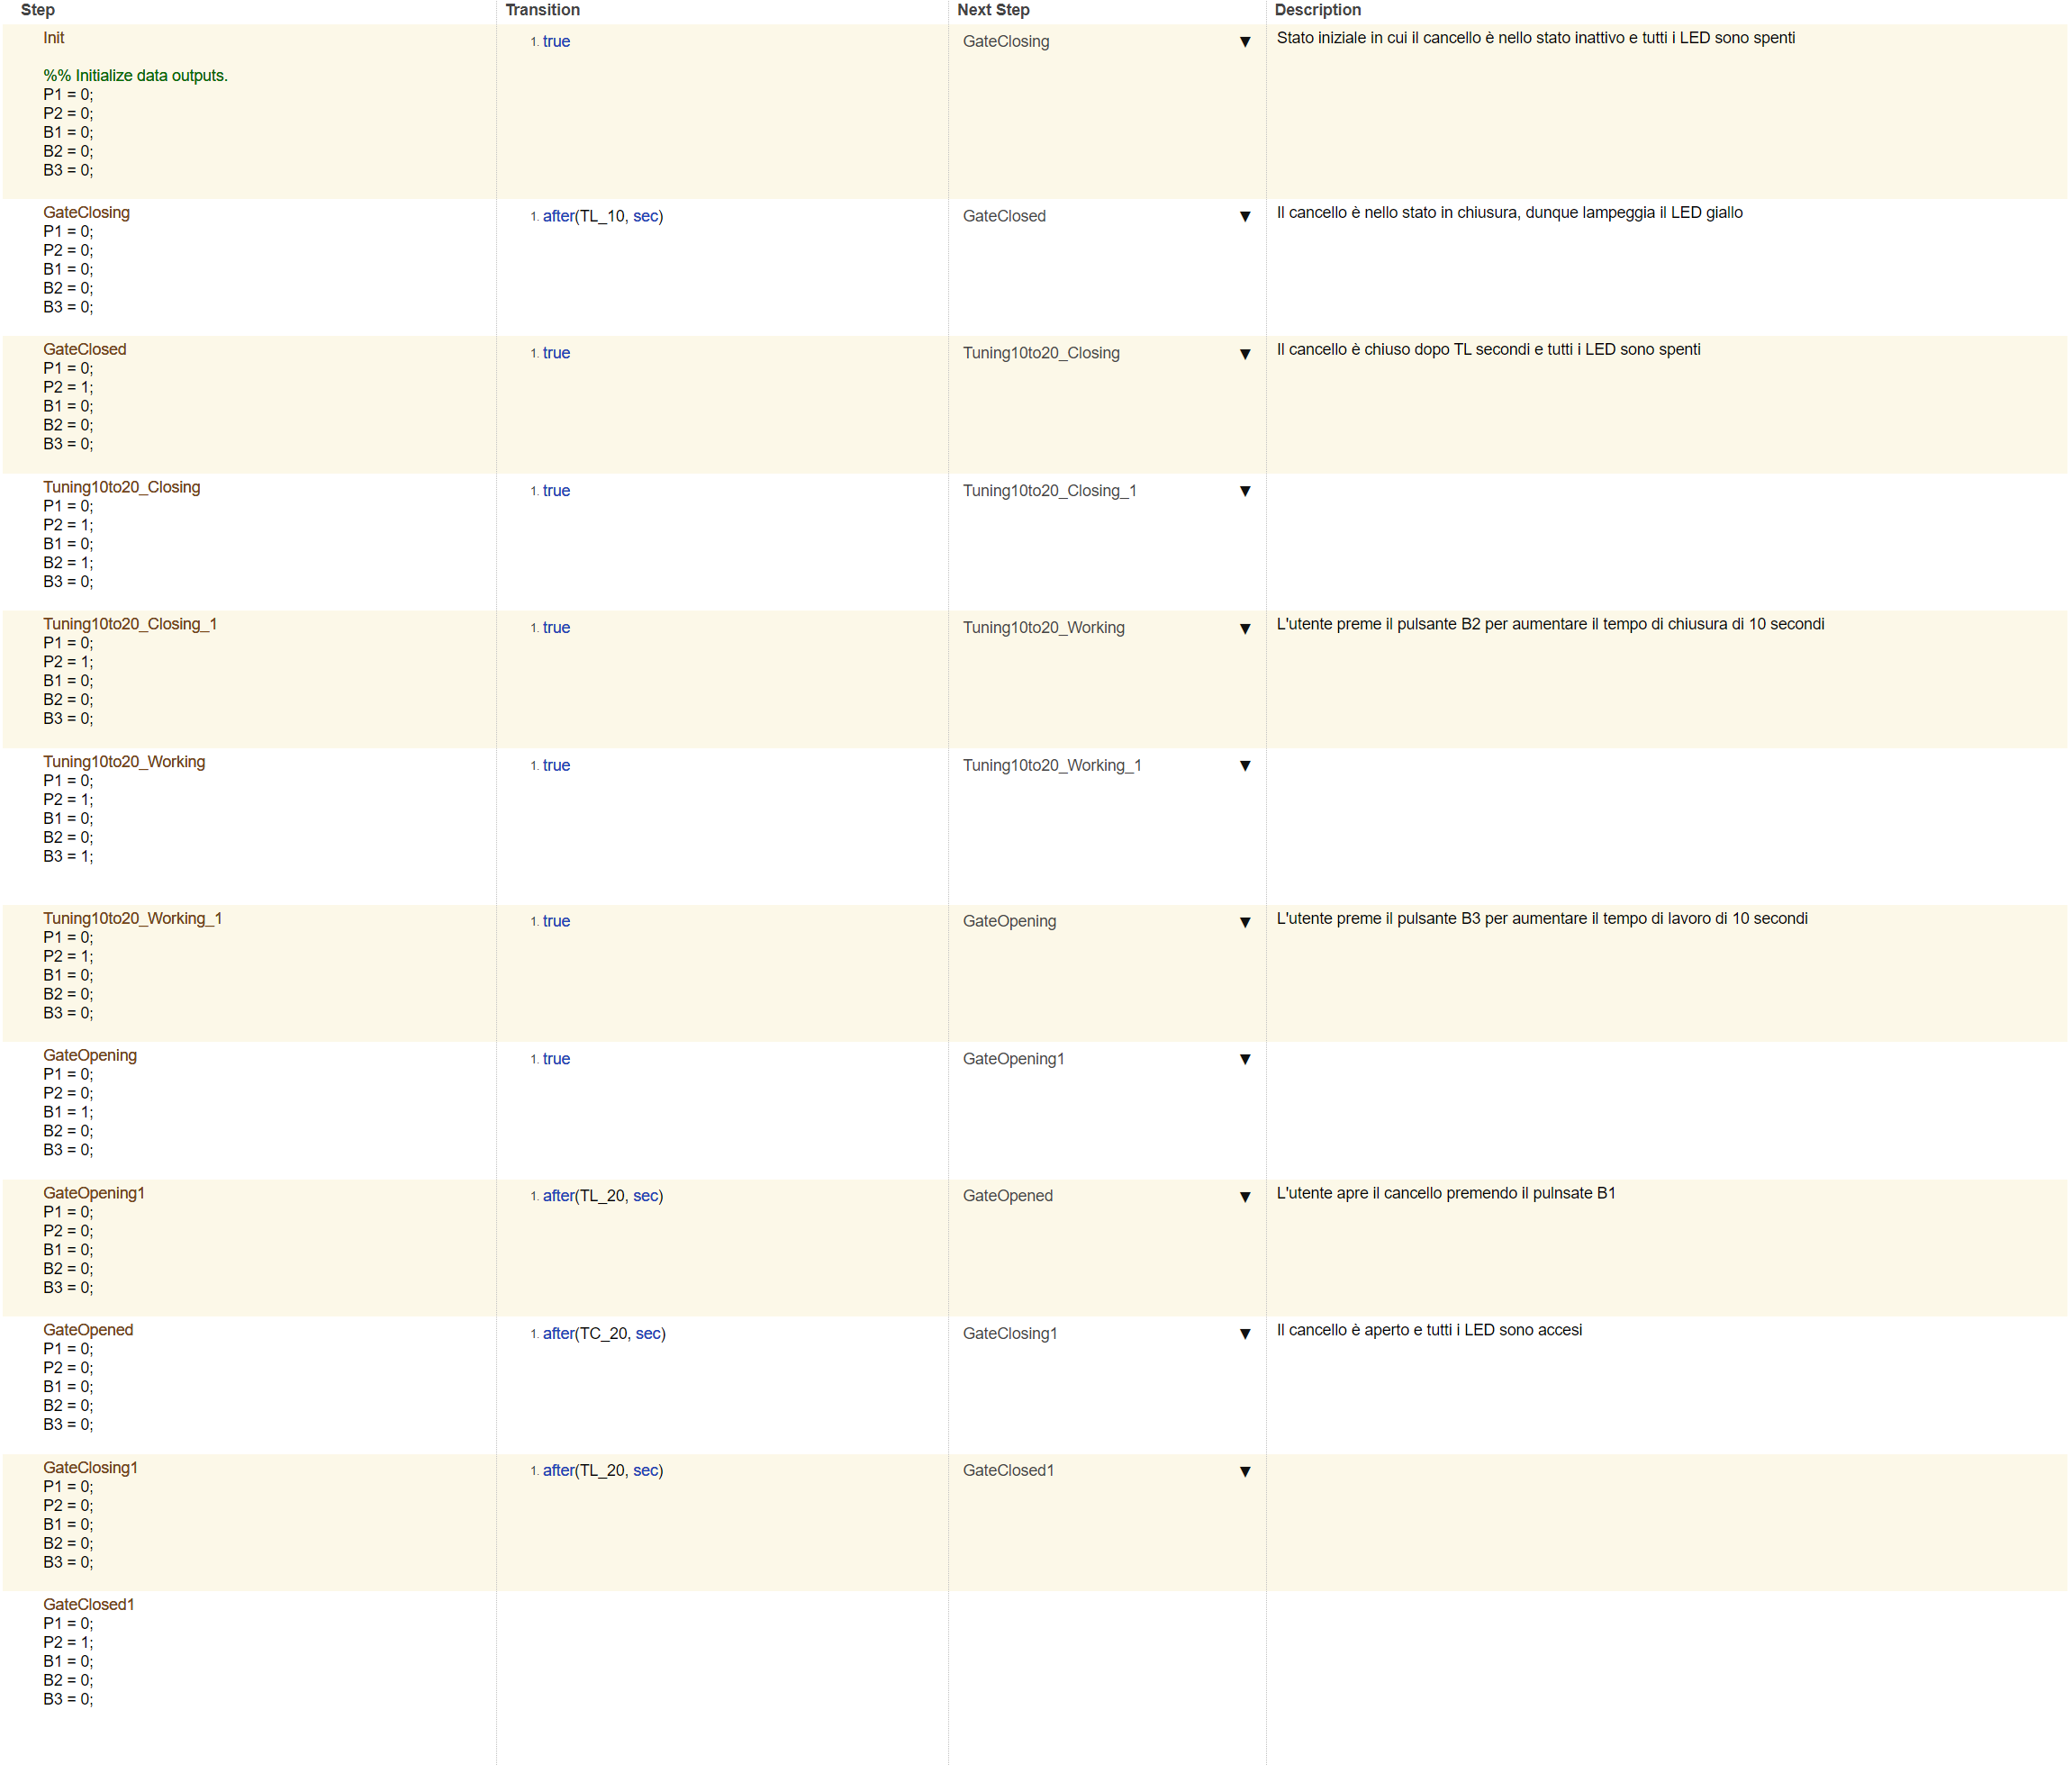
\includegraphics[width=0.9\textwidth]{figures/tuning_closing.png}
            \caption{Test Sequence}
            \label{tuningclos}
        \end{figure}

        \begin{figure}[H]
            \centering
            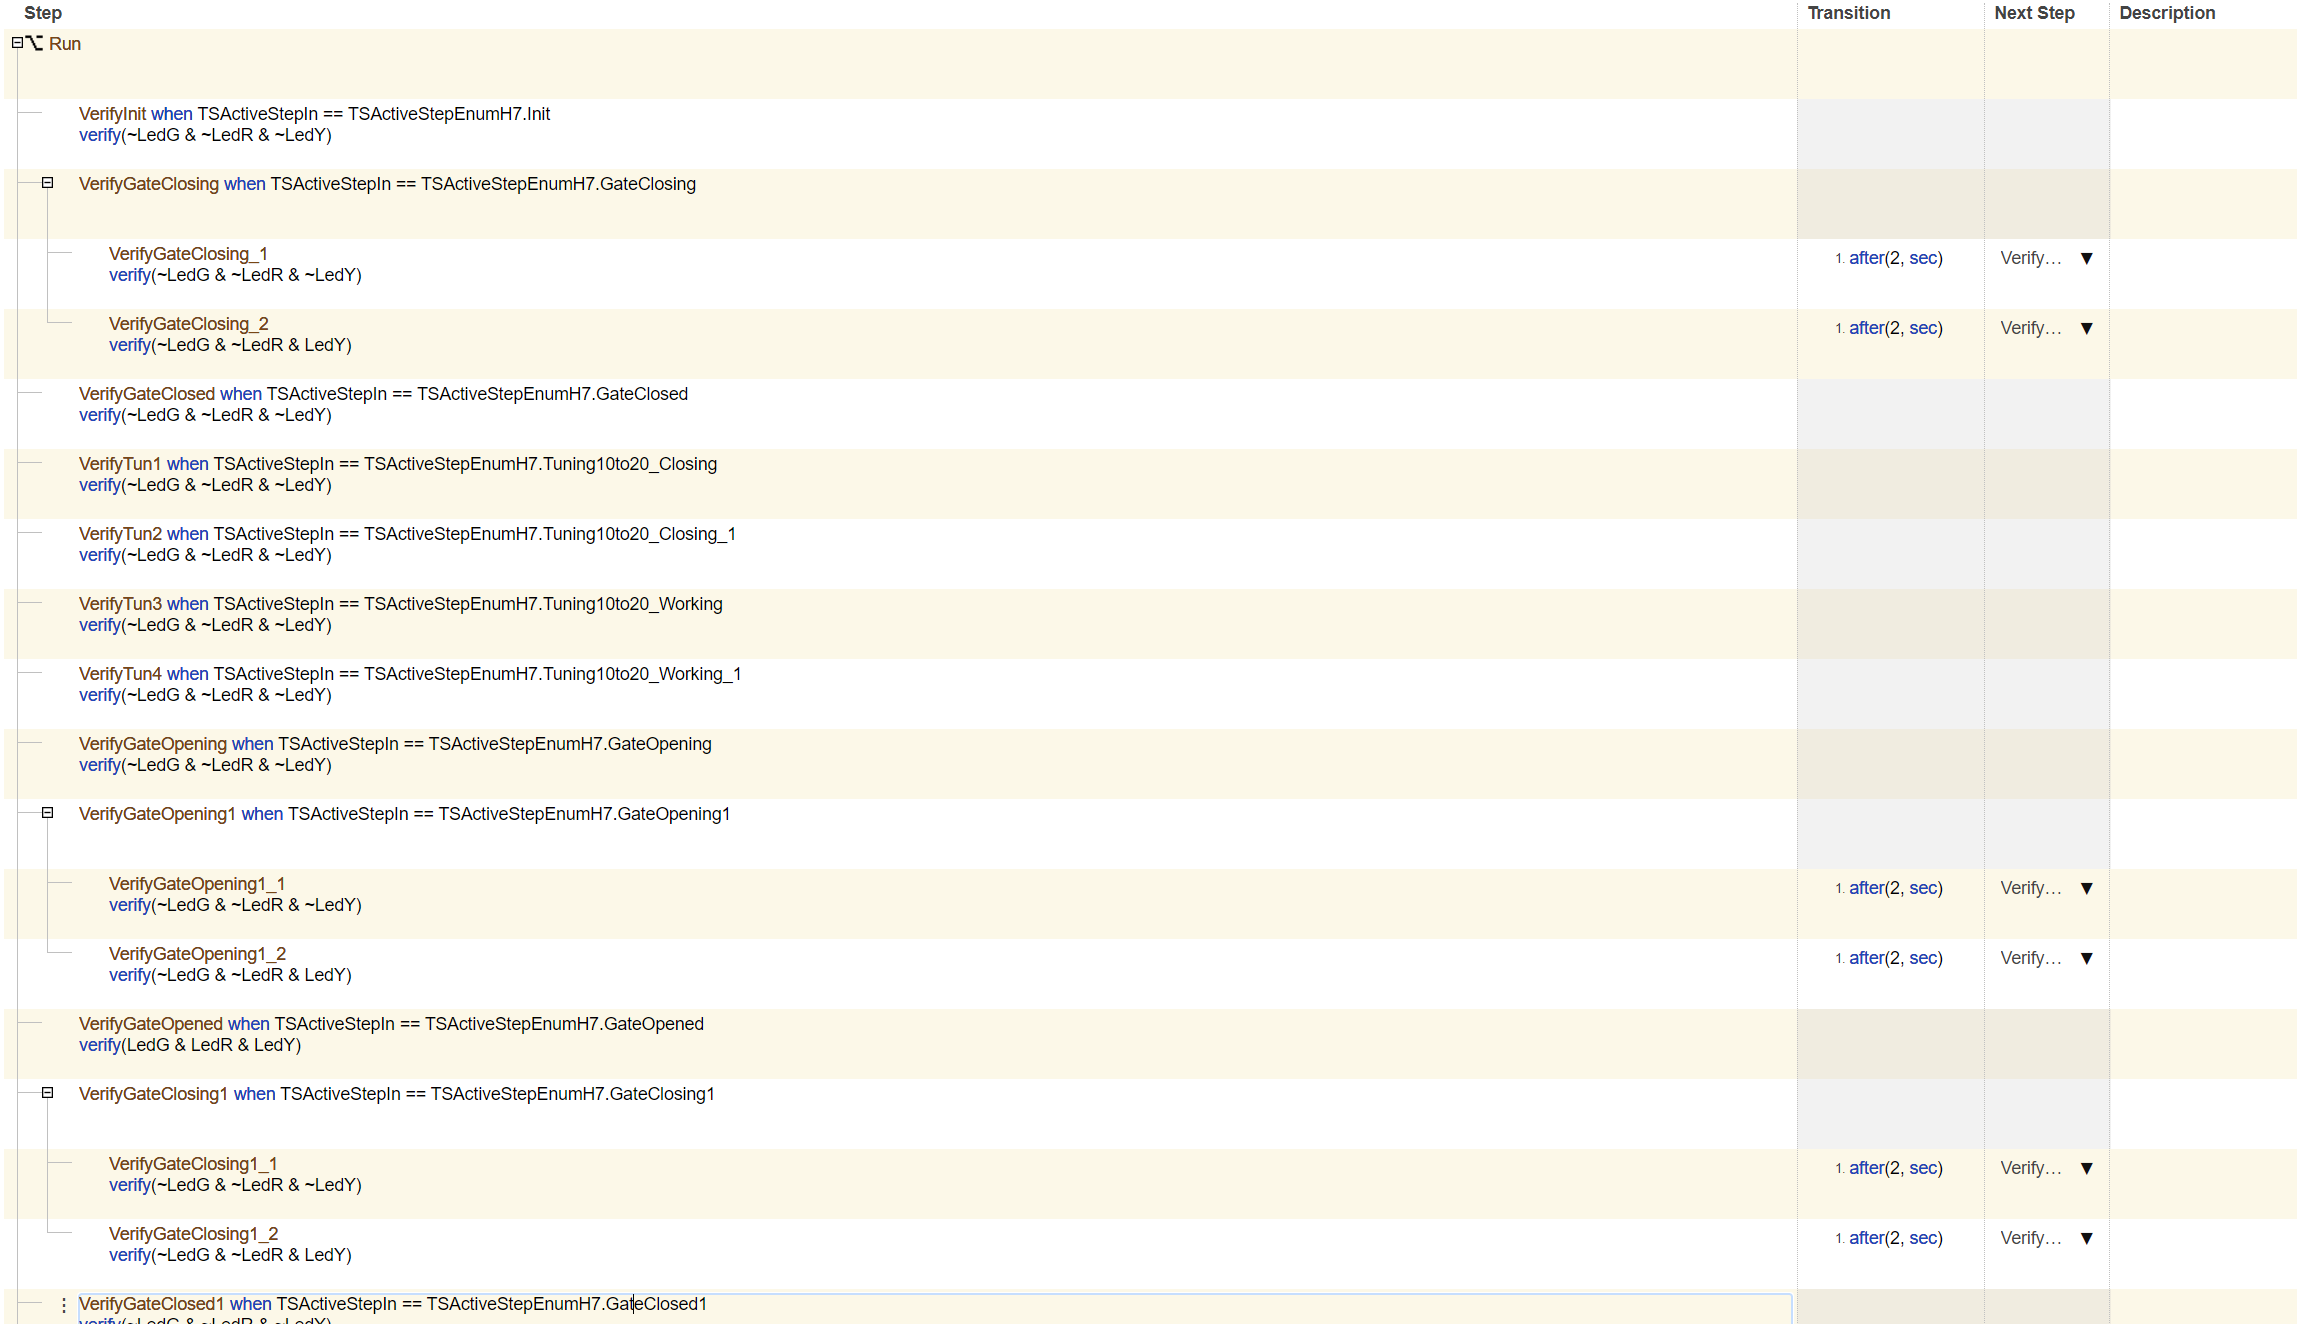
\includegraphics[width=0.9\textwidth]{figures/tuning_closing1.png}
            \caption{Test Assessment}
            \label{tuningclos1}
        \end{figure}


    \section{Regolazione $T_C$ e $T_L$ non nello stato Chiuso}
        Si riporta il test relativo al fallimento della regolazione del tempo di lavoro e del tempo di chiusura mentre il cancello non si trova nello stato \textbf{Chiuso}.
        In particolare, l'utente prova a regolare $T_C$ e $T_L$ premendo i pulsanti $B2$ e $B3$ mentre il cancello si trova nello stato \textbf{Aperto\_Con\_Ostacolo}, dunque la regolazione non avviene con successo e le due variabili precedentemente citate non cambiano il loro valore.

        \begin{figure}[H]
            \centering
            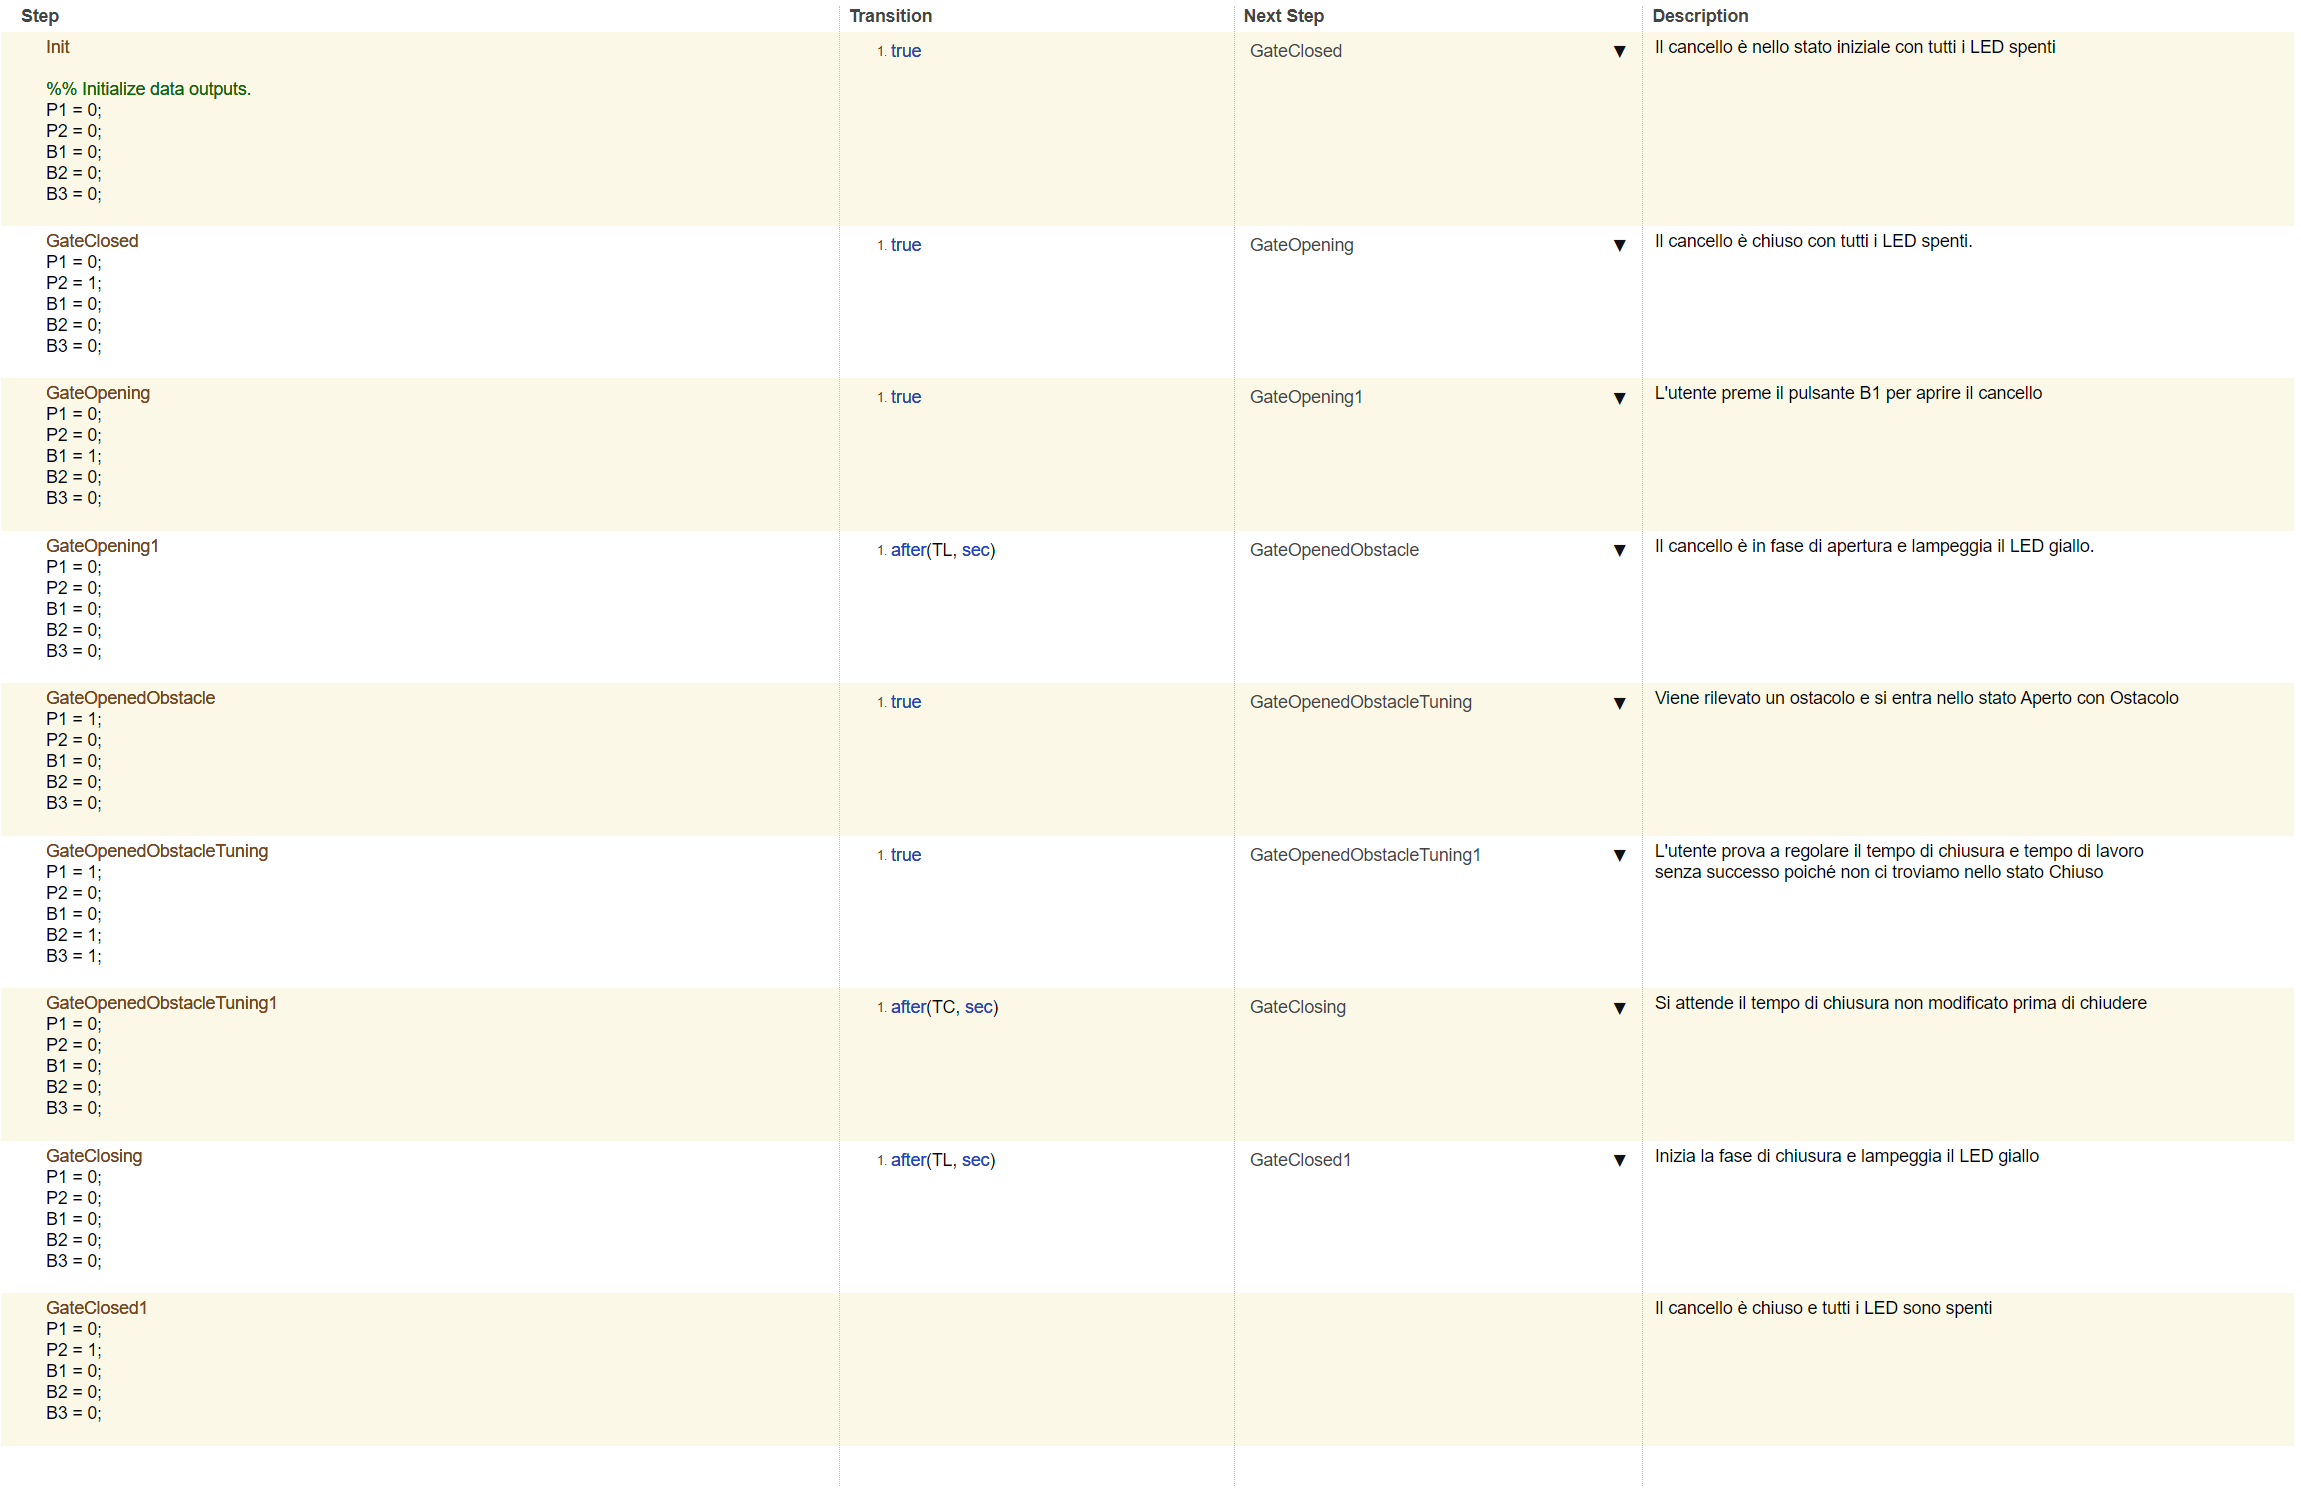
\includegraphics[width=0.9\textwidth]{figures/tuningOB.png}
            \caption{Test Sequence}
            \label{tuningob}
        \end{figure}
        
        \begin{figure}[H]
            \centering
            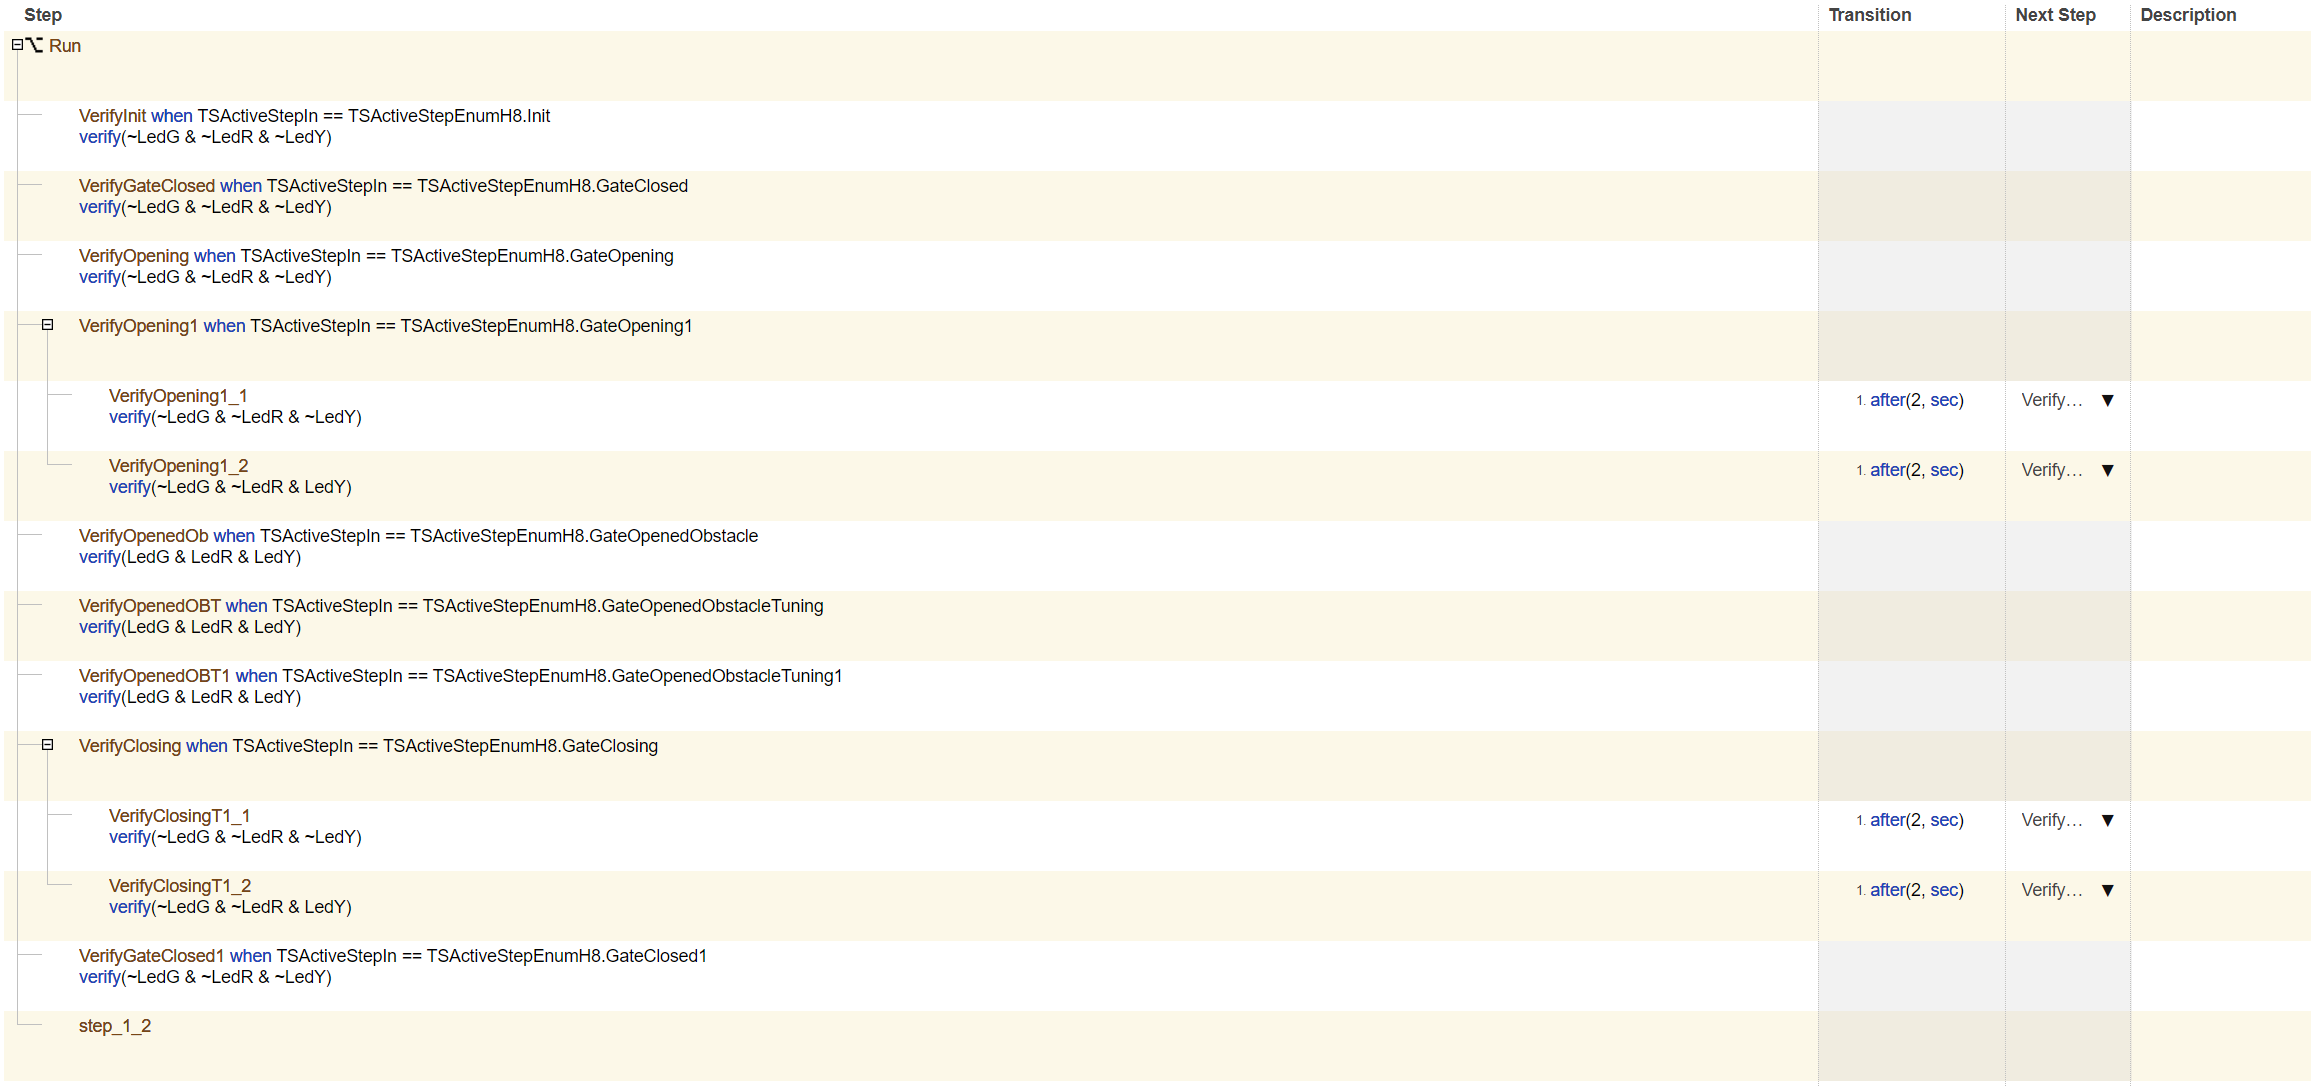
\includegraphics[width=0.9\textwidth]{figures/tuningOB1.png}
            \caption{Test Assessment}
            \label{tuningob1}
        \end{figure}


    \section{Reset del timer durante rilevazione Ostacolo}
    Si riporta il test relativo al reset del timer relativo al lampeggio del LED verde se l'utente preme ulteriormente il pulsante B1. In particolare, se ci si trova nello stato \textbf{Aperto\_Con\_Ostacolo}, se l'utente interagisce col pulsante B1 per chiudere il cancello, il LED verde inizia a lampeggiare per 30 secondi senza alcuna movimentazione del cancello. Il test dimostra che, qualora l'utente dovesse premere di nuovo il pulsante di chiusura (ad esempio dopo soli 5 secondi), il timer si resetta ed il conteggio riparte da 30 secondi.

    \begin{figure}[H]
            \centering
            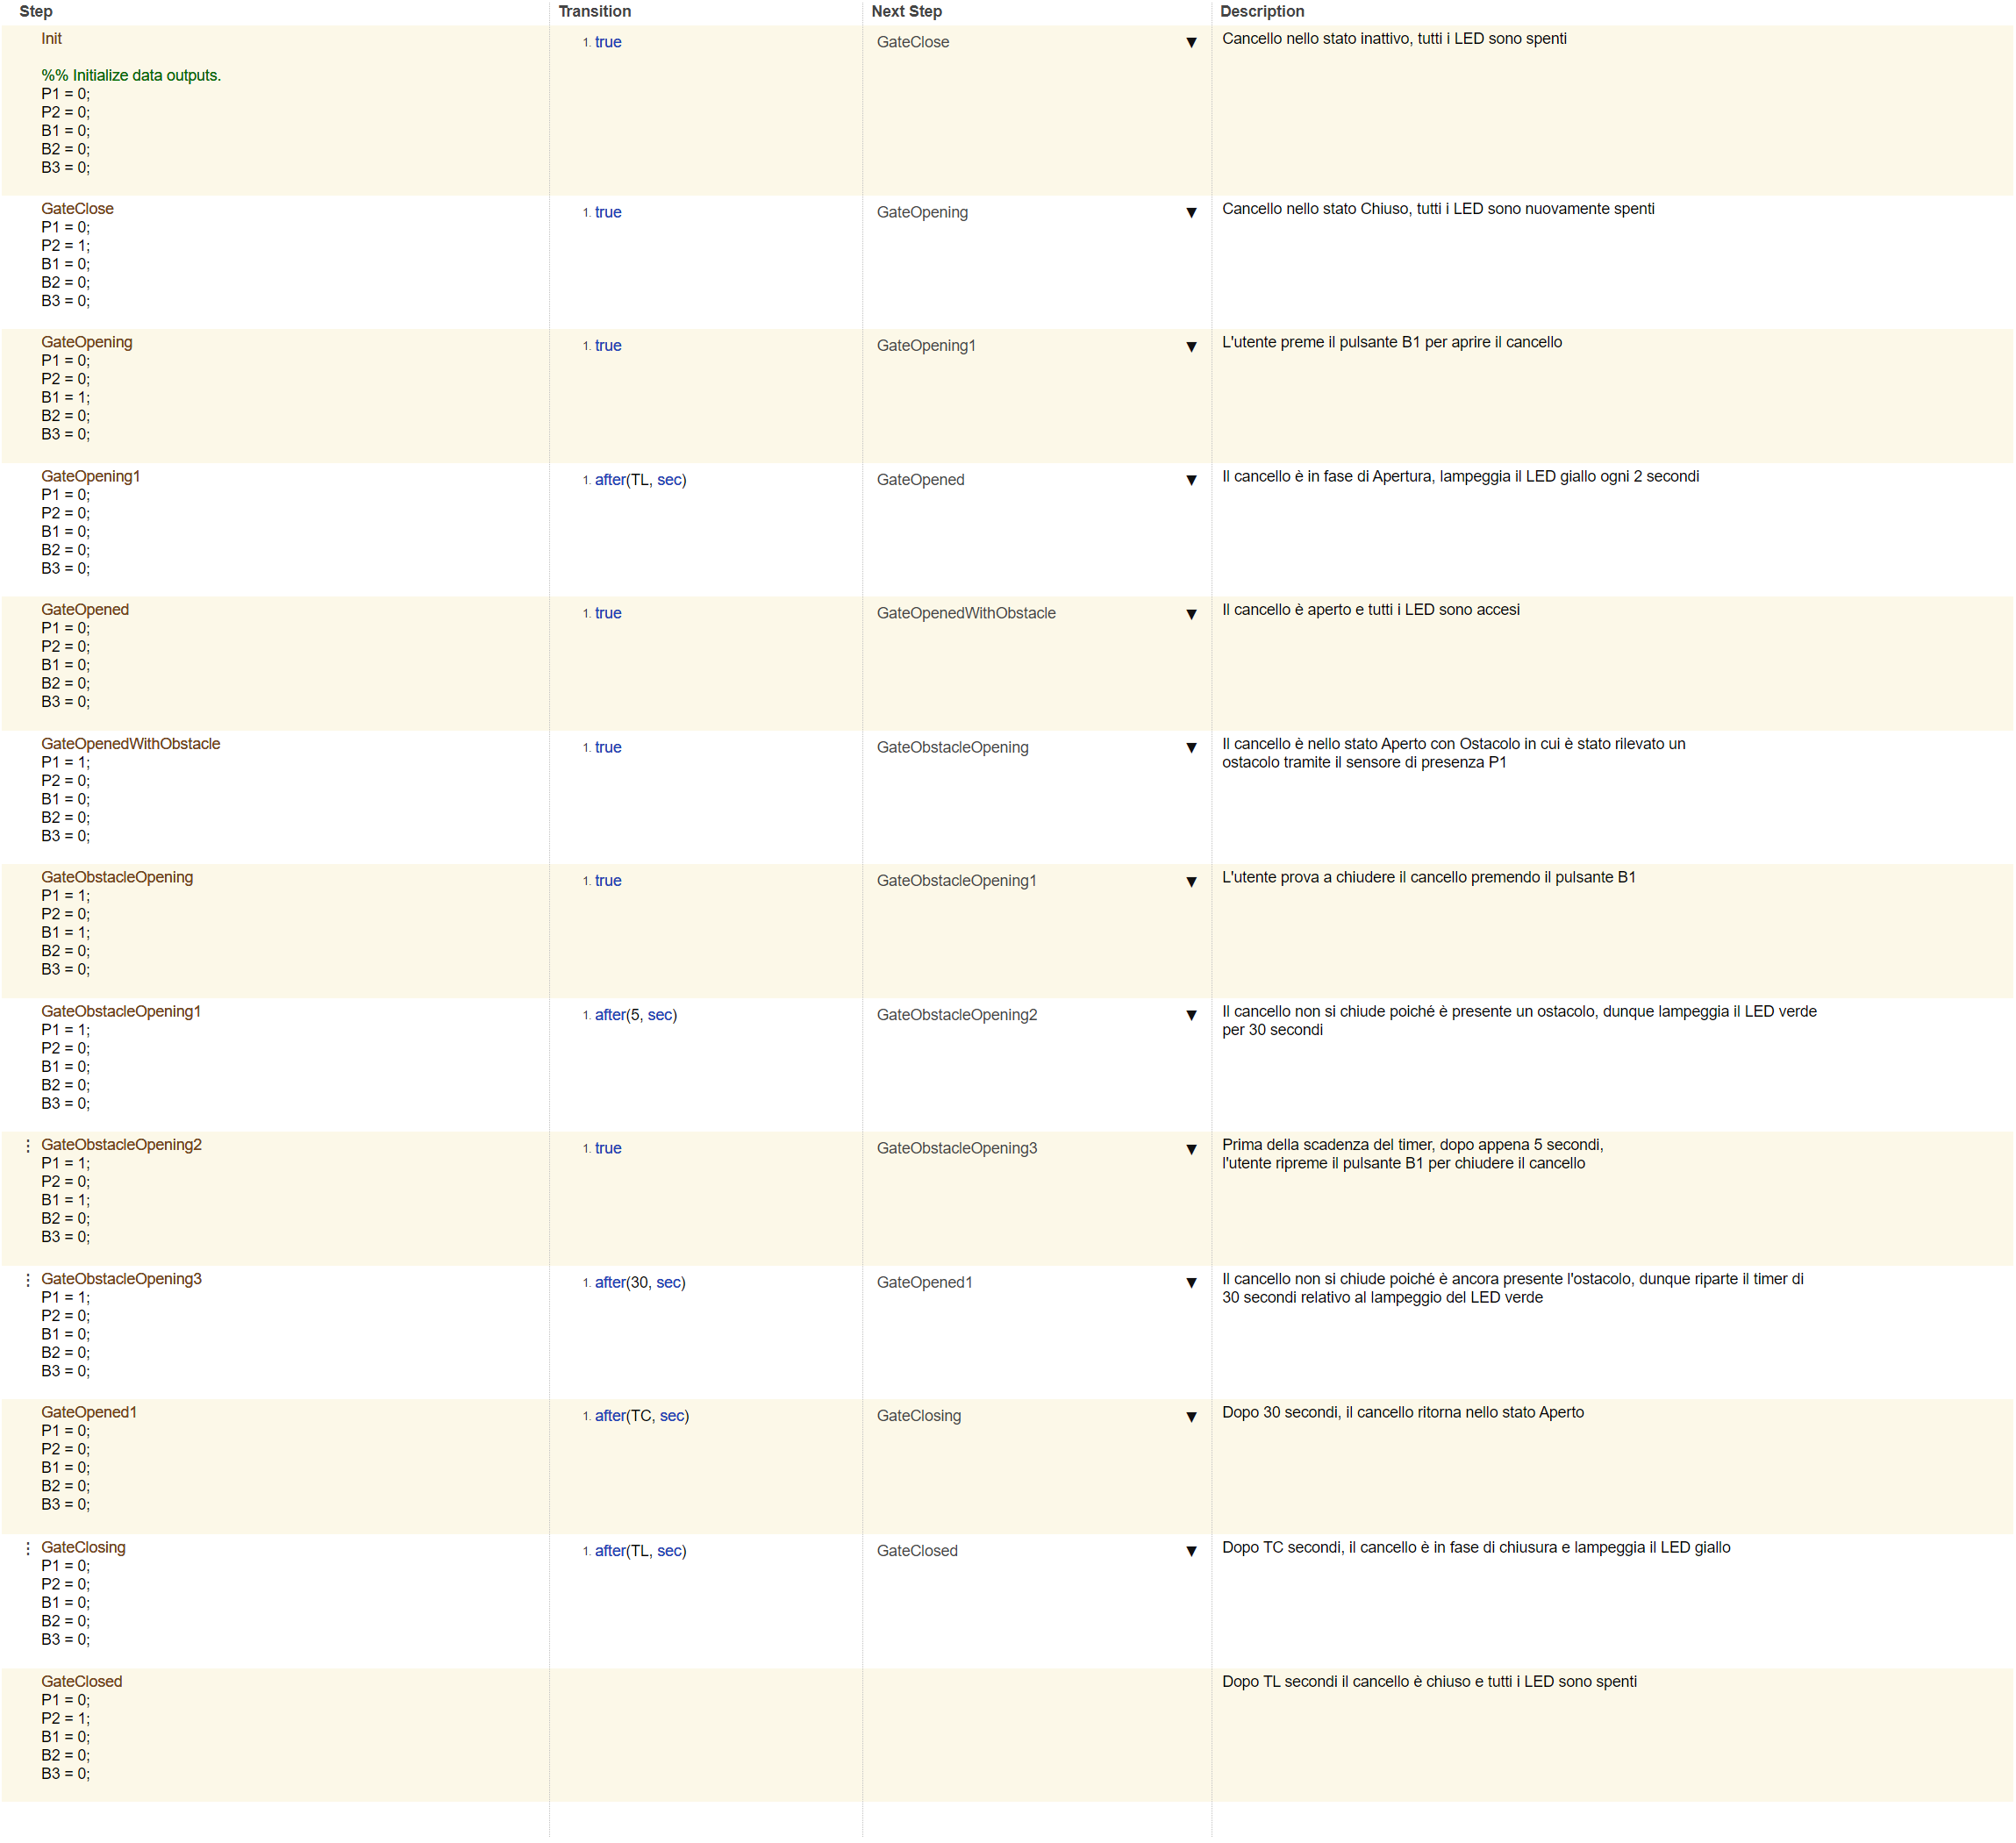
\includegraphics[width=0.9\textwidth]{figures/obstaclerepressed.png}
            \caption{Test Sequence}
            \label{obB1}
        \end{figure}
        
        \begin{figure}[H]
            \centering
            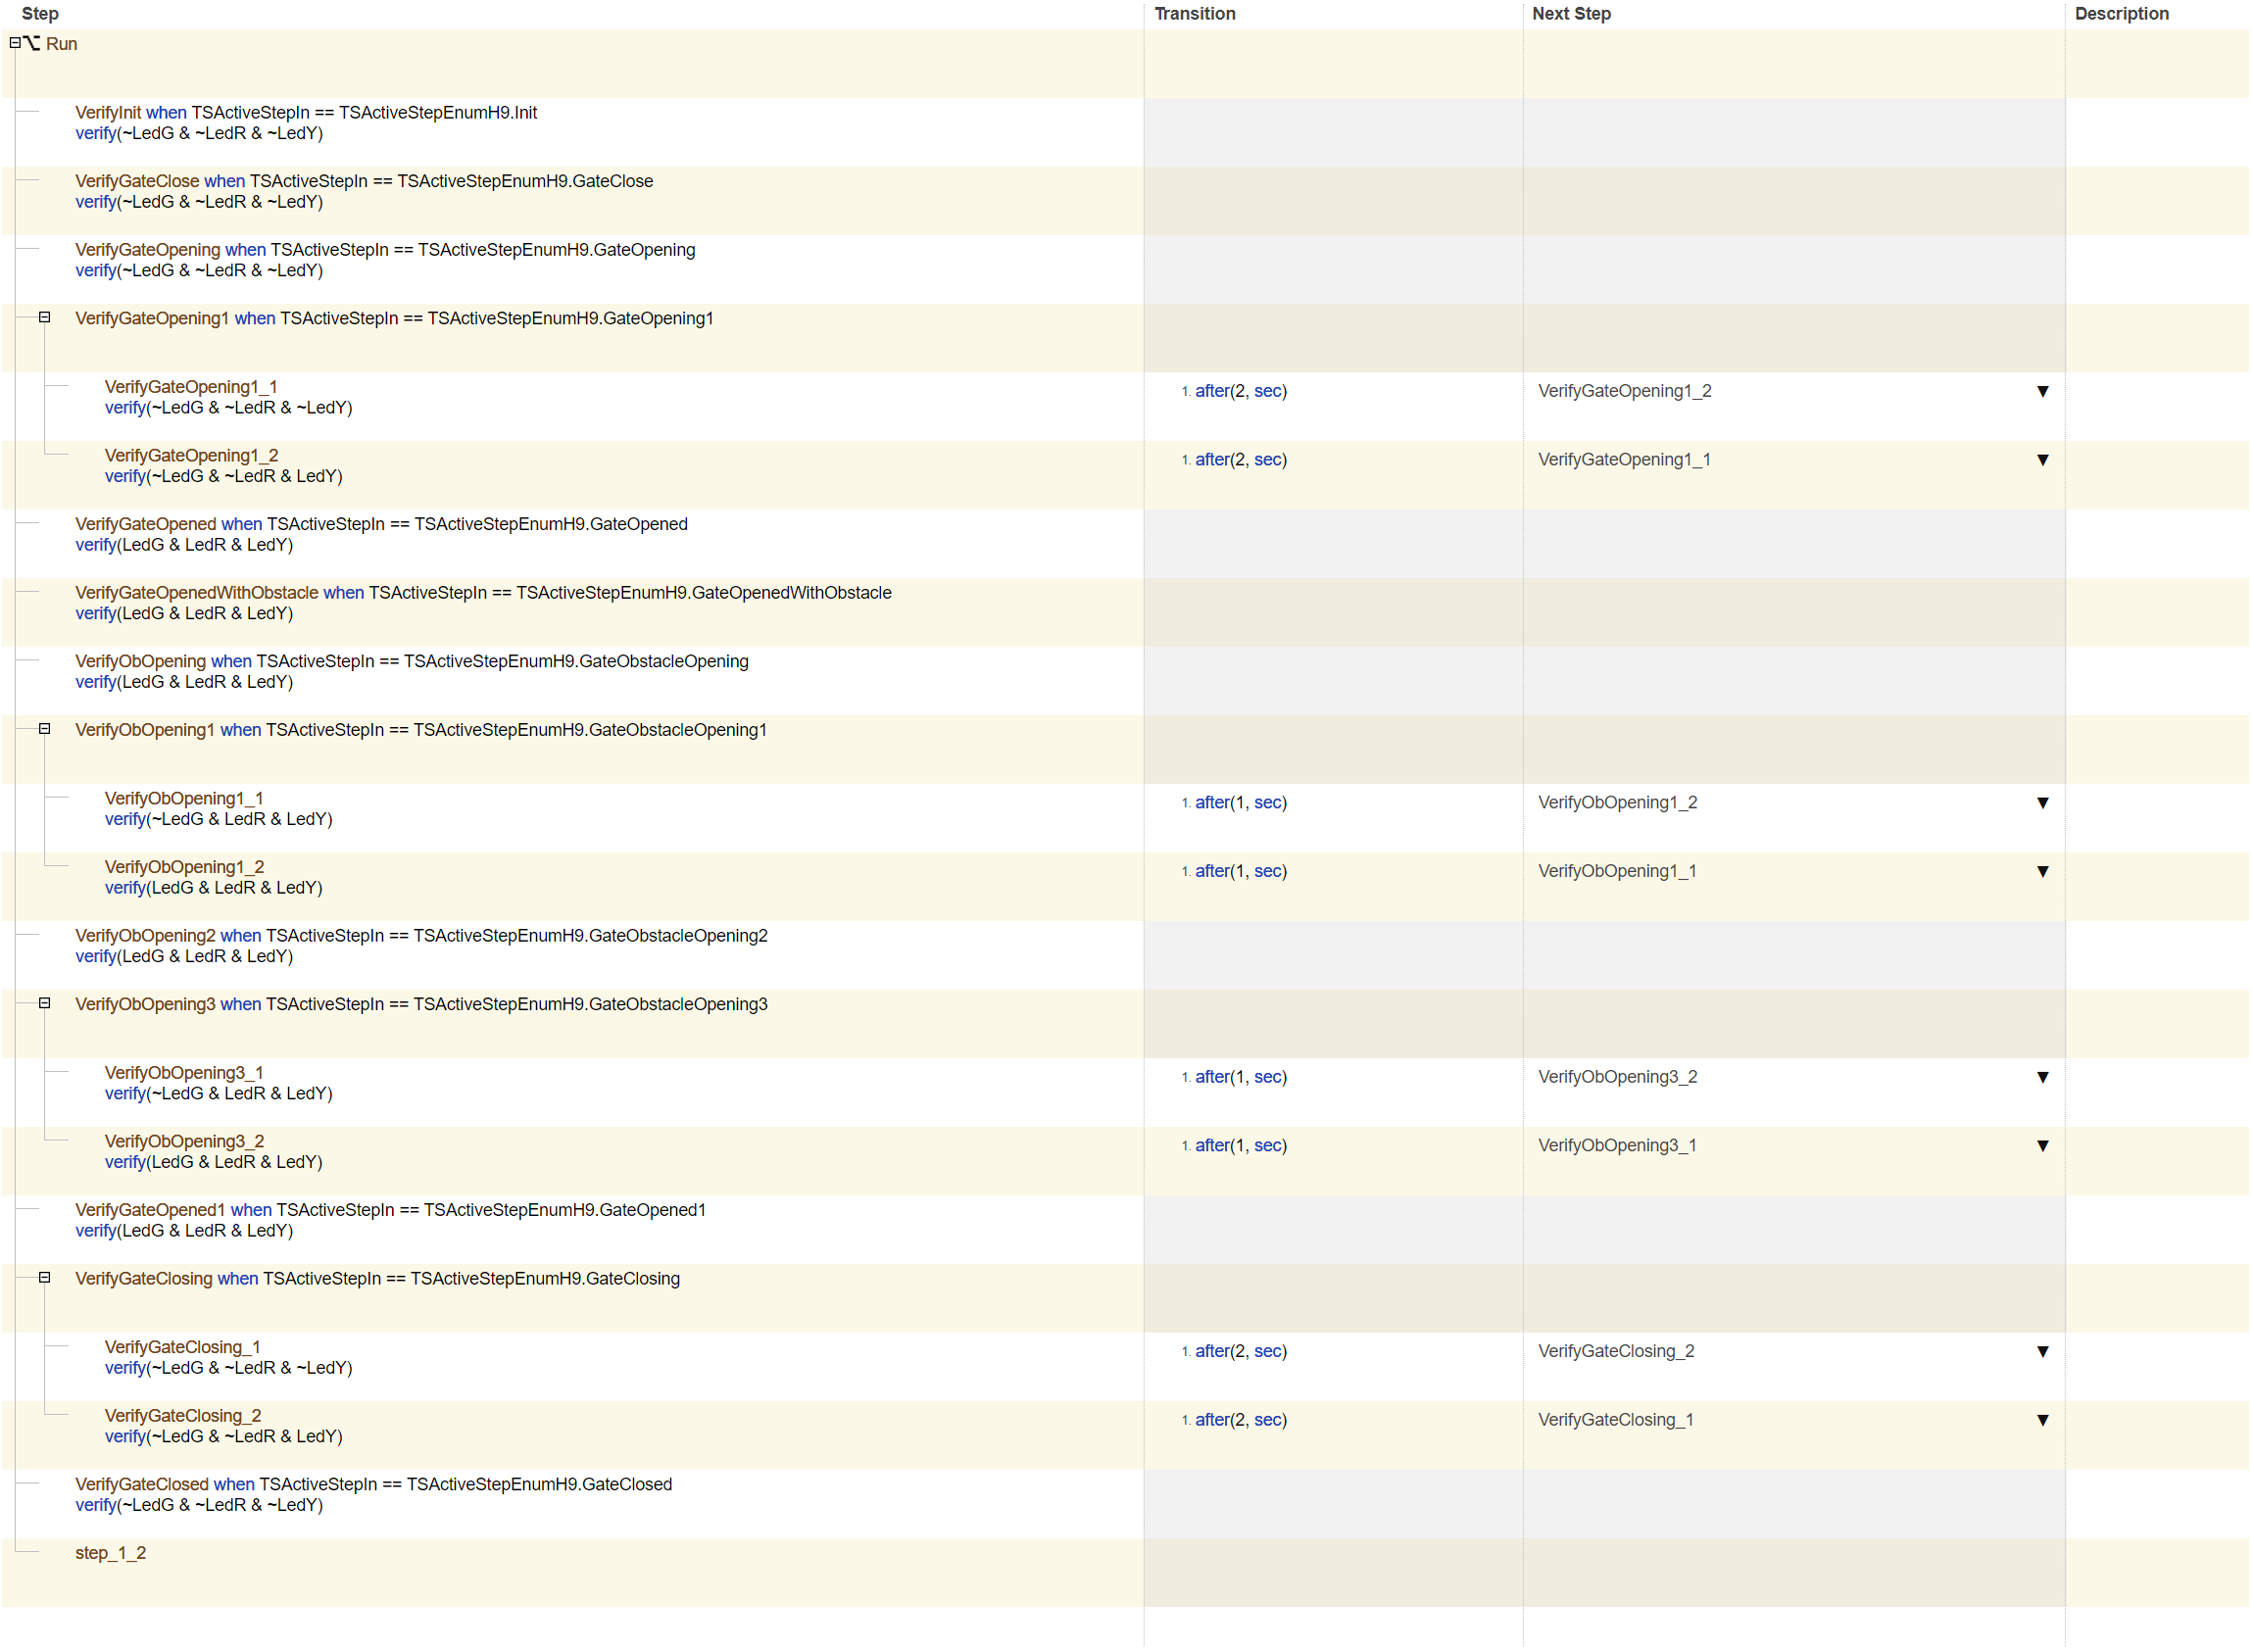
\includegraphics[width=0.9\textwidth]{figures/obstaclerepressed1.png}
            \caption{Test Assessment}
            \label{obB11}
        \end{figure}
    \chapter{Implementazione}
    In questo capitolo si presenterà il codice generato da Matlab, esportato tramite l'add-on Embedded Coder ed il successivo caricamento del firmware sulla scheda STM32 Nucleo  G474RE.

    \section{Realizzazione del circuito}
        \noindent I componenti utilizzati per realizzare il circuito sono i seguenti:
        
        \begin{table}[H]
            \centering
                \begin{tabular}{ | c | c | c | c |} 
                    \hline
                            
                    \textbf{Componente} & \textbf{Pin} \\ 
                    \hline
                            
                    B1 & PC8\\ 
                    \hline
                            
                    B2 & PC6\\ 
                    \hline

                    B3 & PC5\\ 
                    \hline

                    P1 & PC2\\ 
                    \hline

                    P2 & PC3\\ 
                    \hline

                    LedG & PB5\\ 
                    \hline

                    LedY & PB4\\ 
                    \hline

                    LedR & PB3\\ 
                    \hline
                \end{tabular}
            \caption{Tabella variabili Tuning}
        \end{table}

        \noindent In figura \ref{sketch} è presente il circuito realizzato sul software Fritzing.

        \begin{figure}[H]
            \centering
            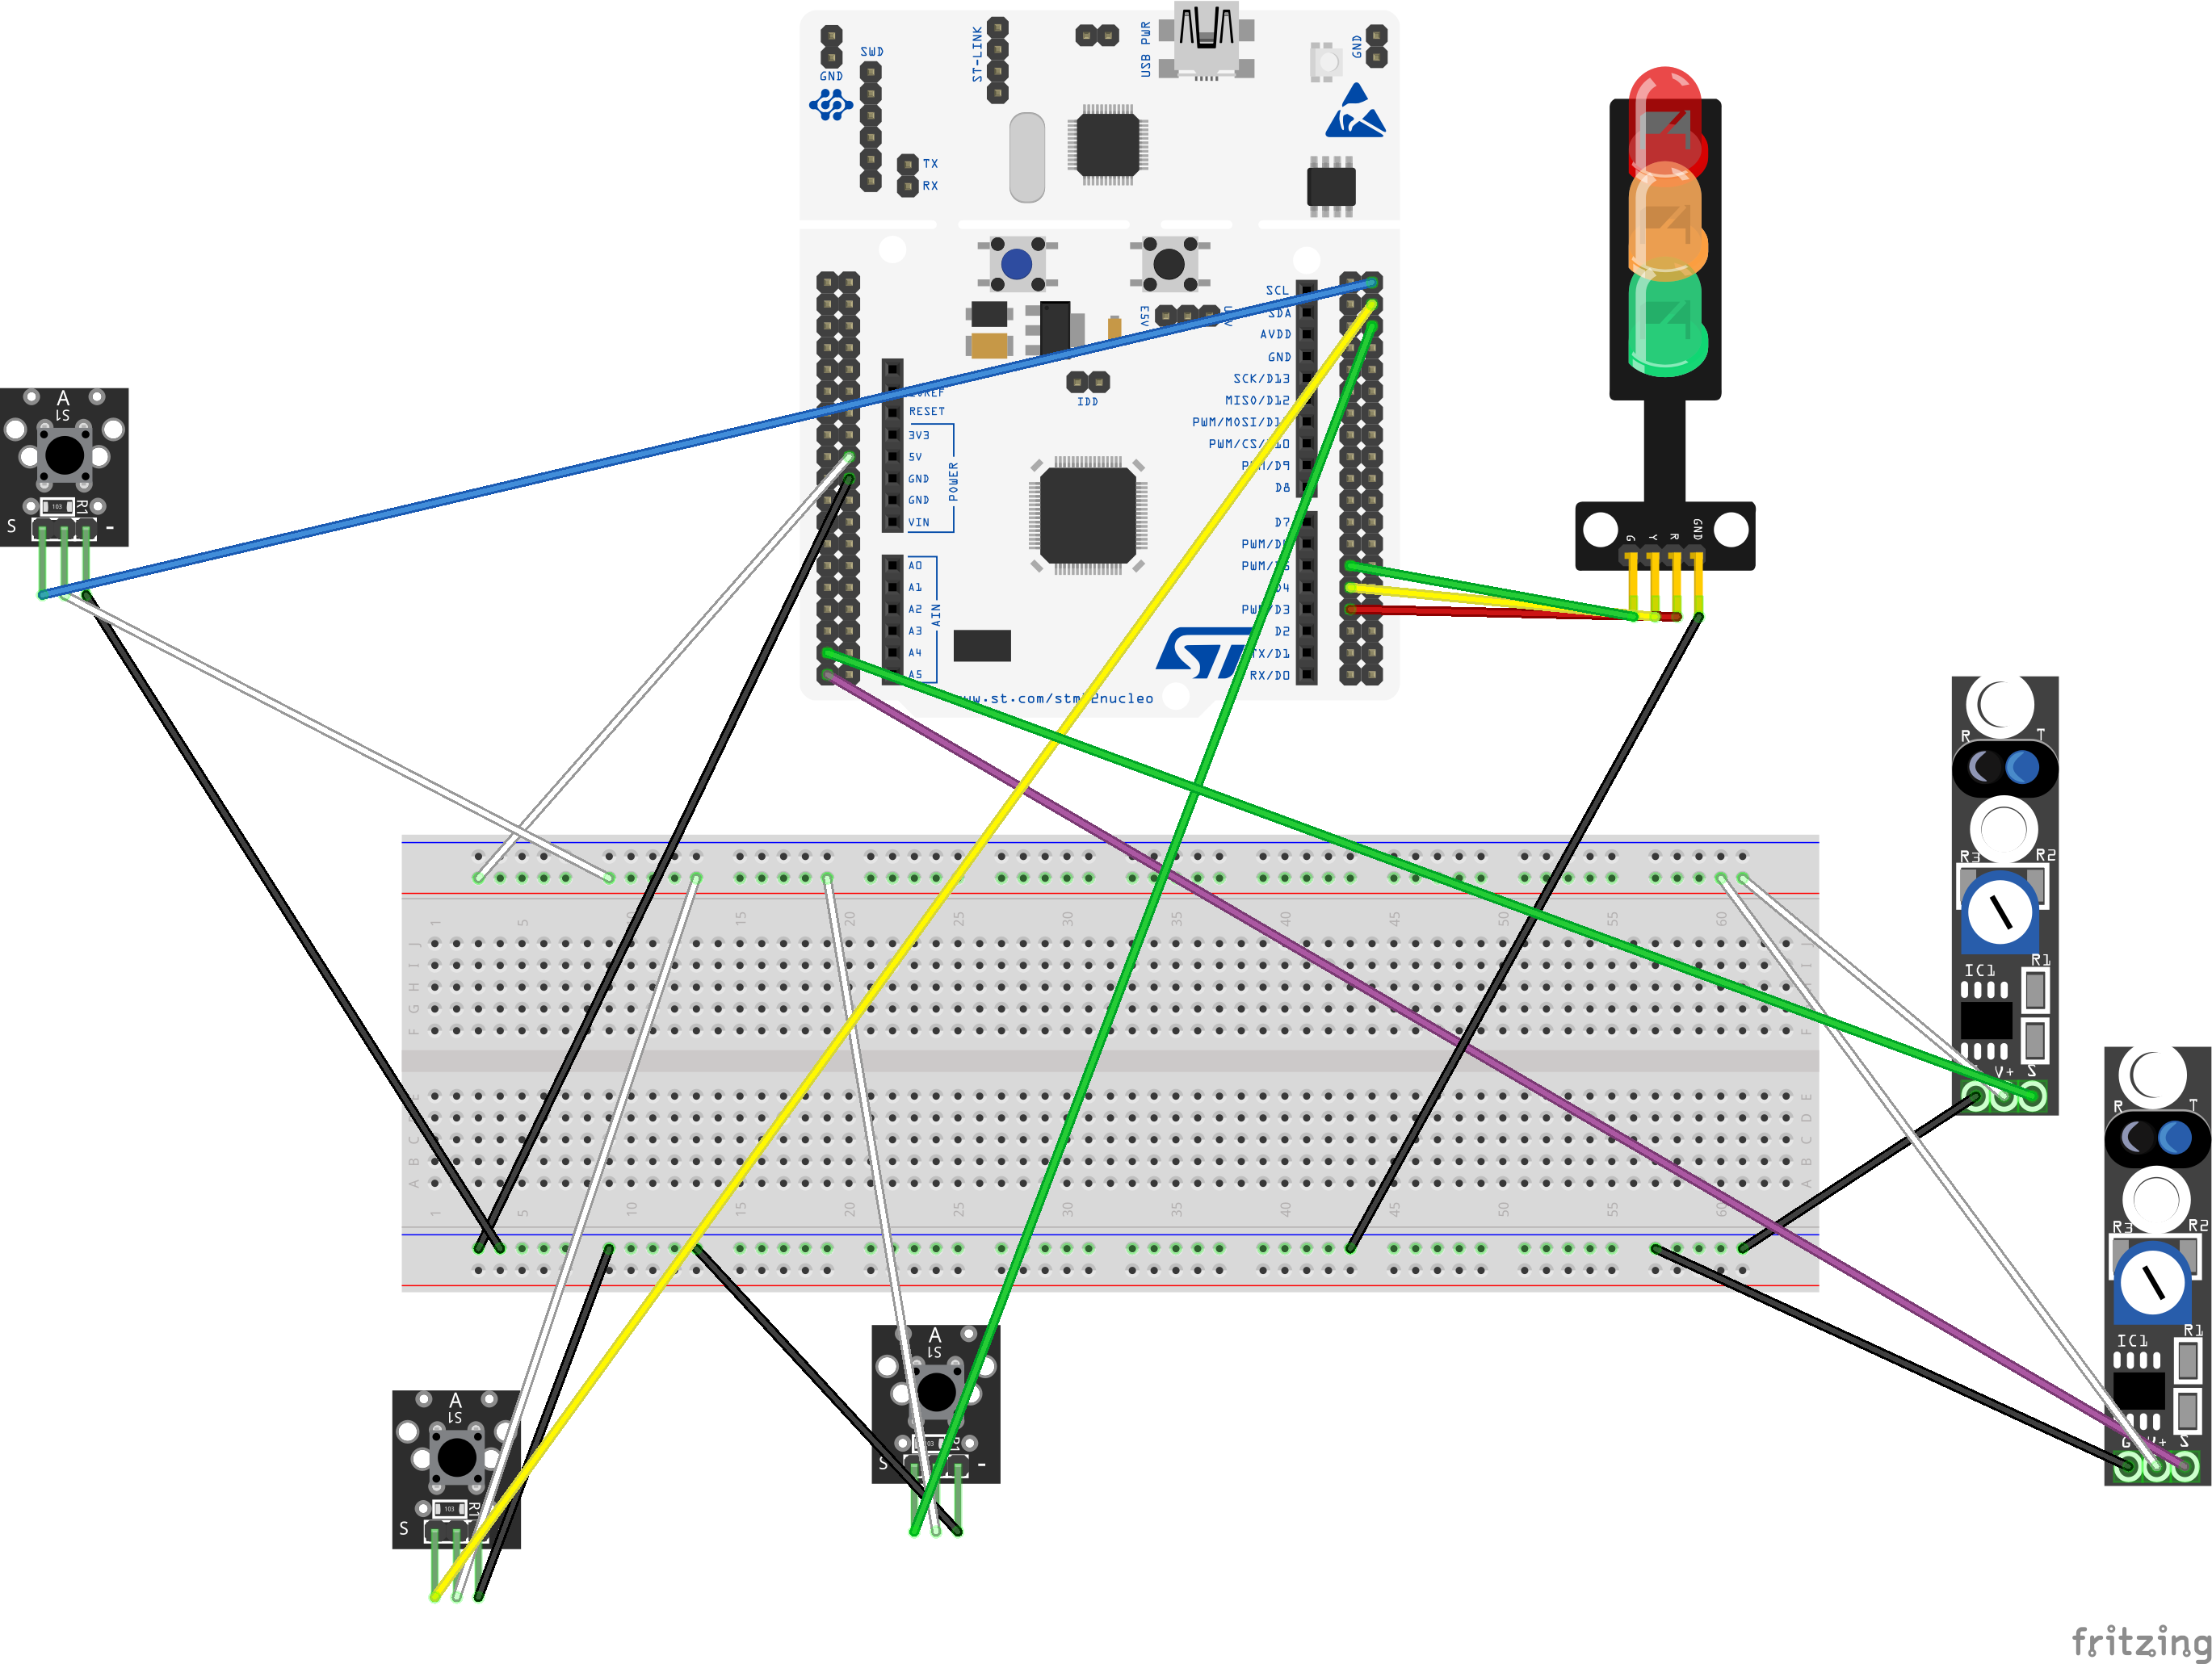
\includegraphics[width=0.9\textwidth]{figures/sketch_bb.png}
            \caption{Circuito su Fritzing}
            \label{sketch}
        \end{figure}


    \section{Codice Sorgente}
        Per generare il codice è stato utilizzato l'add-on \textbf{Embedded Coder}, il quale ha permesso la creazione di tutte le funzioni e variabili necessarie per realizzare l'automa. La creazione del codice sorgente tramite Embedded Coder è una metodologia avanzata che consente di generare codice C e C++ ottimizzato direttamente da modelli Simulink e Stateflow. Questo processo automatizzato non solo accelera lo sviluppo del software embedded, ma riduce anche la probabilità di errori manuali. Embedded Coder offre strumenti potenti per la configurazione del codice generato, permettendo di personalizzare le proprietà e le specifiche per soddisfare requisiti specifici dell'applicazione. Inoltre, supporta l'integrazione con ambienti di sviluppo integrato (IDE) e toolchain per microcontrollori, facilitando il deployment su hardware target.

        Il codice generato è stato importato nell'IDE \textbf{STM32CubeIDE}, dove è stato creato il file main per collegare i componenti fisici della scheda con le variabili create da MATLAB. Questo processo garantisce una sinergia ottimale tra il codice generato automaticamente e l'hardware, assicurando che tutti i sensori, attuatori e altri dispositivi siano correttamente interfacciati e operativi.

        \begin{listing}[!ht]
            \begin{minted}[breaklines=true]{c}
                #include "main.h"
                #include "gpio.h"
                #include "Chart.h"
                void SystemClock_Config(void);
                static void Chart_read_inputs(){
                    rtU.B1 = HAL_GPIO_ReadPin(B1_GPIO_Port, B1_Pin);
                    rtU.B2 = HAL_GPIO_ReadPin(B2_GPIO_Port, B2_Pin);
                    rtU.B3 = HAL_GPIO_ReadPin(B3_GPIO_Port, B3_Pin);
                    rtU.P1 = !HAL_GPIO_ReadPin(P1_GPIO_Port, P1_Pin);
                    rtU.P2 = !HAL_GPIO_ReadPin(P2_GPIO_Port, P2_Pin);
                }
                static void Chart_write_outputs(){
                    HAL_GPIO_WritePin(LedG_GPIO_Port, LedG_Pin, rtY.LedG);
                    HAL_GPIO_WritePin(LedY_GPIO_Port, LedY_Pin, rtY.LedY);
                    HAL_GPIO_WritePin(LedR_GPIO_Port, LedR_Pin, rtY.LedR);
                }
                int main(void)
                {
                    HAL_Init();
                    SystemClock_Config();
                    MX_GPIO_Init();
                    Chart_initialize();
                    while (1)
                    {
                        uint32_t elapsed, start;
                        start = HAL_GetTick();
                        Chart_read_inputs();
                        Chart_step();
                        Chart_write_outputs();
                        elapsed = HAL_GetTick() - start;
                        HAL_Delay(100-elapsed);
                    }
                    }
            \end{minted}
        \caption{Main}
    \label{listing:1}
\end{listing}
    \clearpage
    \phantomsection
\addcontentsline{toc}{chapter}{Indice delle Figure}

\renewcommand{\listfigurename}{\bf Indice delle Figure}
\listoffigures

\end{document}